\documentclass[11pt,a4paper,twoside,openright]{book}
\usepackage[utf8]{inputenc}
\usepackage{pythontex}
\usepackage{minted}
\usepackage{amsmath}
\usepackage{graphicx}
\usepackage{listings}
\usepackage{tabularx, booktabs}
\newcolumntype{Y}{>{\centering\arraybackslash}X}
\usepackage{array}
\usepackage{amsfonts}
\usepackage{subfig}
\usepackage{amssymb}
\usepackage{hyperref}
\usepackage{float}
\usepackage{verbatim}
\usepackage{microtype}
\usepackage{csquotes}
\usepackage[sorting=none,style=numeric,url=false,doi=false,isbn=false,firstinits=true,backend=biber]{biblatex}
\usepackage[parfill]{parskip} % REMOVE INDENTS
\usepackage{wrapfig}
\usepackage{textcomp}
\setcounter{secnumdepth}{5}
\usepackage{longtable}
\usepackage{array}
\usepackage{multirow}
\usepackage{rotating}
\usepackage{lscape}
%\usepackage{chngcntr}%per section figure numbers
\usepackage{array}
\usepackage{setspace}
\usepackage{fancyhdr} % header
\usepackage{epstopdf} %eps to pdf conversion
\epstopdfsetup{outdir=./conv_pics/}
\usepackage{cleveref}
\usepackage[section]{placeins} %stop figures from drifting down into sections where they're not welcome
\raggedbottom
\setlength{\headheight}{13.6pt}%

\setstretch{1.5}
\newcolumntype{P}[1]{>{\raggedright\arraybackslash}p{#1}}
%\counterwithin{table}{chapter}
%\counterwithin{figure}{chapter}
\usepackage[inner=4cm,outer=2cm,top=2cm,bottom=2cm]{geometry}
\addbibresource{library.bib}
\title{Thesis}
\author{Gavin Day}
\date{July 2016}


\begin{document}


\begin{titlepage}

\center


\textsc{\Large Thesis}\\[0.5cm]
\hrule
\vspace{3cm}

{\LARGE \textbf{Identification of Vertebra Characteristics that Determine Different Mechanical Outcomes of Vertebroplasty}\par}  % Title of your document

 \vspace{5cm}

Gavin Day

\vspace{0.5cm}

Supervisors: Professor Ruth Wilcox \& Dr Alison Jones


\vspace{7cm}

\textit{University of Leeds}

\textit{\today}
\vfill

\end{titlepage}


\pagebreak



\tableofcontents
\listoffigures
\listoftables

\pagestyle{fancy}
%\renewcommand{\chaptermark}[1]{\markboth{\MakeUppercase{#1}}{}}
%\renewcommand{\chaptermark}[1]{ \markright{#1} }

\fancyhf{}
\fancyhead[LE,RO]{\thepage}
\fancyhead[LO,RE]{\chaptermark }
\chapter{Literature Review}

\section{Introduction}
\subsection{Spine}\label{spine}

The human spine is a complex structure that has a host of biomechanical
functions. At each level, there are three joints (a disc and two facet
joints) which, along with two vertebrae, muscle and ligamentous tissue
form a functional unit. The functions of the spine are: to protect the spinal cord,
 to provide stability and mobility, and to allow the transmittance of
movement of the upper and lower extremities.

The spinal column (Figure \ref{fig:spine}) consists of 24
articulating vertebrae and nine fused vertebrae, divided into five regions. These regions consist of seven
cervical, 12 thoracic, five lumbar, five fused sacral and three to five
fused coccygeal vertebrae, which all vary in size, shape and curvature.

\begin{figure}[hbt]

\centering
  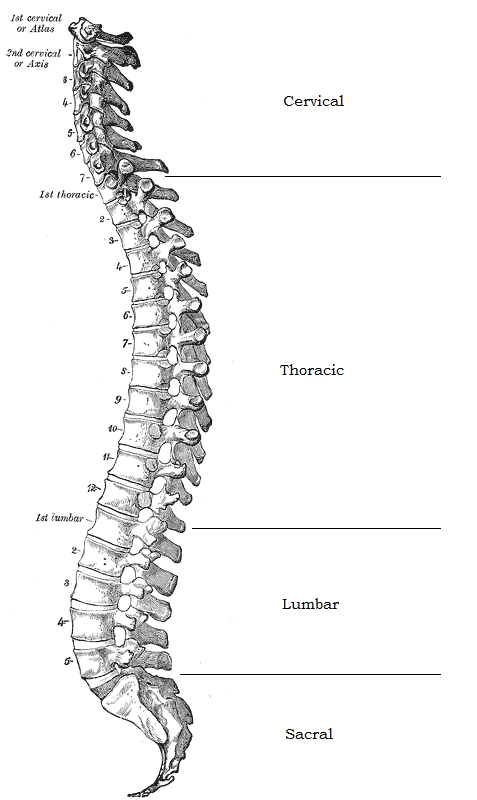
\includegraphics[width=7cm]{images/spine.png}
  \caption{Curvature of the vertebral column with the four regions labelled.
Adapted from \cite{Gray1918}.}
\label{fig:spine}
\end{figure}




The curvature of the spinal column features lordosis (concave curvature, when viewed from the posterior)
in the cervical and lumbar regions and kyphosis (convex curvature) in
the thoracic and sacro-coccygeal regions. It has been postulated that
the curvature exists to increase rotational stability -- moving mass
away from the centre line increases the centre of inertia about the
skull-pelvis axis. The change in curvature during gait cycle reduces the
loads on the skull due to absorption of energy in the tendons and
musculature of the surrounding areas. The curvature is created by
vertebral geometry in the thoracic and sacral regions, while in the
cervical and lumbar regions the curvature is created by the
intervertebral disc being wedge shaped.

\subsection{Vertebrae}\label{vertebrae}

Vertebrae vary greatly between each region and gradually within them.
Generally, vertebrae consist of the vertebral body on the anterior portion and the neural arch on the posterior portion along with pedicles and bony processes (Figure \ref{fig:vertebra}).

The vertebral body has a similar structure to long bones, with a
low-density trabecular structure internally, with a more dense cortical
shell. Due to approximately 80 percent of the compressive load of the
spine being carried by the vertebral body \cite{Adams2005}, the trabeculae are orientated
vertically to aid load transfer with horizontal trabeculae providing
resistance to compressive buckling. Especially in older patients, often
with osteoporosis, the vertebral body can be subject to vertebral
fracture, more commonly on the anterior portion, causing anterior collapse and a wedge shape when viewed from the side \cite{Adams2005}.

Vertebral bodies vary between level in terms of cross sectional area,
height and strength, with the axial strength of vertebrae increasing
from approximately 1300 N at the third cervical level to over 8000 N at the fourth lumbar level \cite{Stewart2006}. Similar variations have been found in the bone mineral density (BMD) \cite{yoganandan2006}, with the BMD varying
with the loads they are expected to carry. While a reduction in BMD is most often associated with osteoporosis, similar increases in the risk of fracture are attributed to metastatic bone disease.

\begin{figure}[hbt]
\centering

  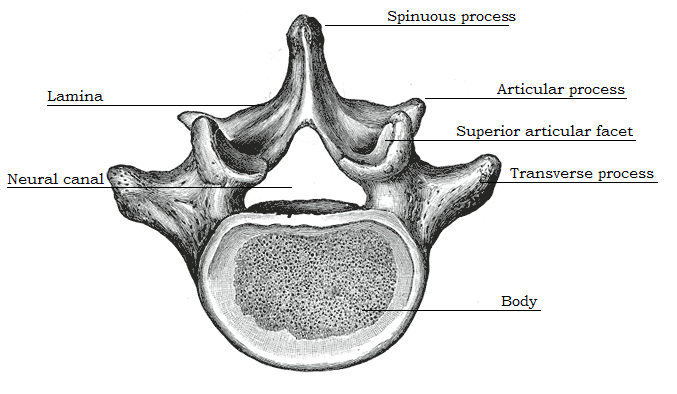
\includegraphics[width=10cm]{images/vertebra.png}
  \caption{Superior view of a lumbar vertebrae, with key features labelled.
Adapted from \cite{Gray1918}.}
\label{fig:vertebra}
\end{figure}


The posterior region of the vertebrae consists of two pedicles, followed
by the neural arch and processes. The spinous and transverse processes
allow for greater leveraging by the muscles and ligaments while the
superior and inferior articular facets of neighbouring vertebrae form
the facet (zygapophysial) joints.

Vertebrae at different levels have differing structures to permit their
required role. Cervical vertebrae are considerably smaller and lighter
than vertebrae at other levels due to the reduced weight they are
required to carry (the head and neck, and forces from stabilising
muscles). One identifying feature is the foramen transversarium lateral
to the vertebral body which allows for the passage of the vertebral
artery and vein \cite{panjabi1991cervical}.

The thoracic vertebrae vary substantially through T1 to T12 with the
size of the vertebral body gradually increasing and the pedicles
changing in orientation and shape. The addition of adjoining ribs
through the thoracic region greatly increase the stiffness of the
section due to the ligaments and costovertebral joints.

The lumbar vertebrae carry the greatest load of the spinal regions
\cite{Stewart2006} and consequently have the lowest height to width ratio
\cite{Manohar1992}.
The end-plates (at the top and bottom of a given vertebra) of this region are in general parallel, suggesting that
the lordosis originates from the disc shape rather than the vertebrae.

The sacral vertebrae are fused to form the sacrum which are followed by
three to four elements that form the coccyx and fuse in adulthood.
\section{Vertebral Fractures \&
Vertebroplasty}\label{vertebral-fractures-vertebroplasty}

\subsection{Vertebral Fracture Types}\label{vertebral-fracture-types}

The two most frequent types of vertebral fracture are the compression
fracture and the burst fracture. These types originate from different
conditions of both the intact vertebrae and the loads applied. To
examine the type of fracture, the vertebra is often categorised into
three columns from a sagittal view, with the columns being: the anterior
, middle and posterior regions \cite{Denis1983}.

\subsubsection{Compression Fractures}\label{compression-fractures}

A vertebral compression fracture (VCF) is a failure of the vertebral
body under the anterior column with the middle column remaining intact,
a feature unique to this type of fracture \cite{Denis1983}. Such fractures can
also be identified through compression of the cancellous bone and lack
of fragmentation. The two main types of VCF are anterior and lateral,
with the mechanism being anterior flexion and lateral flexion
respectively. These types can be further divided based on whether the
superior or inferior end-plate experienced failure, however failure of
the superior end-plate is more common \cite{Denis1983}. Radiographically, the
anterior
height of the vertebral body is reduced with no visible change or damage
to the posterior region of the vertebral body \cite{Denis1983}, although
occasionally in juvenile and osteoporotic vertebrae the damage is
limited to end-plate impaction \cite{Magerl1994}. A more extreme case
is a
vertebral body collapse, found in osteoporotic spines, where
occasionally fragments of bone are produced which can violate the spinal
canal especially when both end-plates are impacted (such cases are
treated as burst fractures) \cite{Magerl1994}.

\begin{figure}[hbt]
\centering
  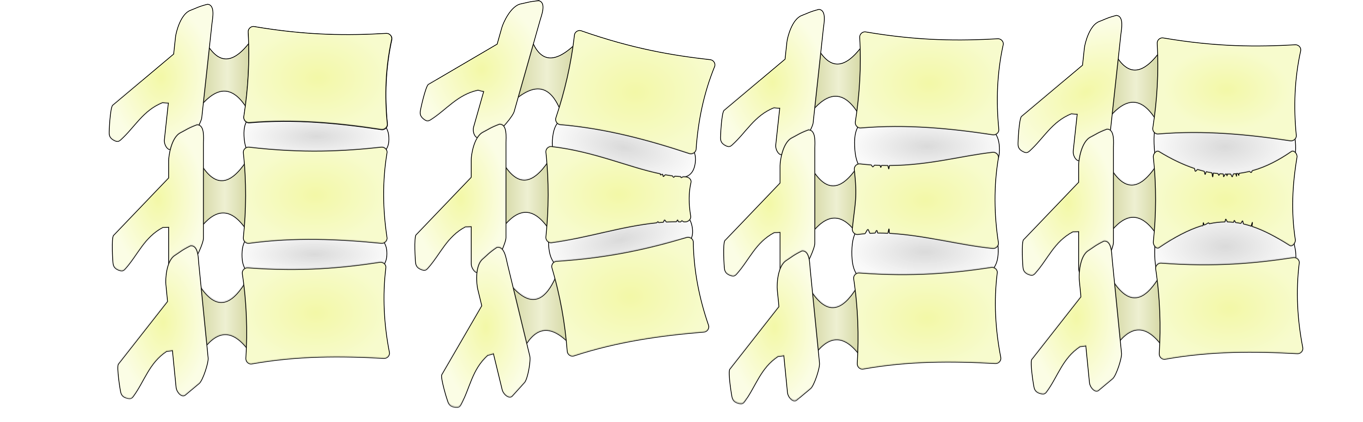
\includegraphics[width=\textwidth]{Chapters/Chapter_Lit_images/type_of_fracture}
  \caption{Types of VCF. Left: Intact FSU. Left-Mid: Anterior wedge fracture. Right-Mid: Posterior wedge fracture. Right: Vertebral body collapse. }
\end{figure}





A study of 132 anterior VCFs by Denis \cite{Denis1983} found that the
distribution of fractures favoured the upper lumbar region (L1 was
considerably more common) and mid-thoracic (T7 most common in the
thoracic region). Lateral VCFs accounted for only 16 of the 148 VCFs,
which were all found to occur in the lumbar region except one case.

\subsubsection{Demographic}

Patients suffering from vertebral compression fractures (VCFs) can
experience severe pain for extended amounts of time, dramatically
changing daily activities in addition to the pain, through reducing the lower vital capacity and forced expiratory volume when compared to patients without
such fractures \cite{Mathis2001}. Mortality rates were also reported to increase
with
VCFs in women, with the rate increasing further with the addition of
more fractures \cite{Mathis2001}.

Due to VCFs occurring most commonly through the loads applied to the
spine exceeding the axial strength of the vertebral body, the
demographic of sufferers is dominated by those with osteoporosis or
tumours within the vertebrae \cite{Mathis2001}. The occurrence of osteoporosis
is
usually age related with the frequency of VCF increasing from 25 percent
of postmenopausal women to 40 percent in women aged 80 years old in the
United States \cite{Studies2006}. However, as discussed by Melton \& Kallmes
\cite{MeltonIII2006}, there is difficulty in defining VCFs due to the number
of
systems developed to define them and the lack of a clear gold
standard for classification. This study found that the prevalence varied from 7\% to 19\%
for women in the age range of 50-80 years depending on the method by
which the fracture was defined and 4\% to 17\% for men in the same age
range. The prevalence of osteoporotic VCFs in women was found to be
twice that of men in an age-adjusted study \cite{Cooper1992}.

VCFs due to tumour infiltration into the vertebrae is another subset of
patients and was the motivation for the first image guided percutaneous
vertebroplasty procedure in 1984 \cite{Burstein1987}, however it is
difficult
to
assess the rate of such occurrences. The increasing ability to treat
osteolytic metastases and myeloma, leave more patients open to vertebral
collapse. This is further increased by possible secondary osteoporosis
induced by the treatment of malignant lesions \cite{Mathis2001}. However,
specific
pathologies and trauma account for a mere 3\% and 14\% respectively of
all clinically relevant fractures \cite{MeltonIII2006}.

\subsection{Risk Factors}\label{risk-factors}

Many of the risk factors of VCFs are the same as osteoporosis due to
their linked nature and can be categorised into potentially modifiable
and non-modifiable risk factors \cite{Studies2006}. Non-modifiable factors
include
age, gender, Caucasian race and history of existing fractures;
modifiable factors include insufficient physical activity, calcium and
vitamin D deficiency and alcohol and tobacco use \cite{Studies2006}.

\subsection{Diagnosis}\label{diagnosis}

Approximately two thirds of VCFs are undiagnosed \cite{Cooper1993} due to back
pain often being regarded as a consequence of aging and not reported by
patients. Care is often required to ensure that pain is directly related
to a VCF and not another spinal entity such as facet arthropathy,
herniated disc and spinal stenosis \cite{Mathis2001}. Indicators for Percutaneous Vertebroplasty (PVP) are
often
described as pain localised to the area, which lacks suggestions of
nerve or cord compression and includes an increase in pain under
weight bearing \cite{Mathis2001}. Vertebral pain for 1-6 weeks that fails to
reduce
after oral analgesics has also been defined as an indicator \cite{Diamond2006}.

Due to the strong relationship between BMD and bone strength, with
stronger vertebrae exhibiting a higher BMD \cite{Moro1995}, dual energy
X-ray
absorptiometry (DEXA) or quantitative CT can be used to predict
vertebral fractures. Increasingly the ability to assess the bone
structure at the clinical level gives a greater ability to clinicians to
predict fractures more accurately, due to BMD effectively being a
surrogate for the trabecular structure.

\subsection{Vertebroplasty}\label{vertebroplasty}

The main group of patients that receive
PVP are those with either osteoporotic VCFs or those with tumour
infiltration. Early use of PVP was limited to those patients who
responded poorly to conservative treatments, including analgesics, bed
rest, physical therapy and in some cases bracing \cite{Mathis2001}. However due
to
the low complication rate of PVP, indication of an osteoporotic VCF is
often enough and helps to reduce further compression of the vertebral
body \cite{Diamond2006}. PVP consists of the injection of bone cement into the
vertebral body from the posterior side of the body. The addition of
cement into an osteoporotic, fractured vertebral body allows
stabilisation of the fracture with the aim of reducing pain for the
patient.

\subsubsection{Vertebroplasty Procedure}\label{vertebroplasty-procedure}

Performing vertebroplasty requires careful monitoring during cement
injection and cannula placement; this is carried out with the use of
fluoroscopic guidance, which helps to limit the possibility of
extravasation (cement leakage from the vertebral body). Biplane fluoroscopy is often used, allowing the procedure
to be carried out more rapidly, while single plane fluoroscopy requires
checking both lateral and anteroposterior projections \cite{Mathis2001}.

There are three common approaches to the vertebral body: transpedicular,
parapedicular, and oblique, shown in Figure \ref{fig:vpapproach}.
Transpedicular
vertebroplasty
provides
a
route into the vertebral body through the pedicle, which acts as a
tunnel reducing the risk of dural puncture. Depending on patient
vertebrae size and level, the pedicle may be insufficient to allow
passage of the vertebroplasty needle and hence other approaches may be
required. The transpedicular approach also often requires injection from
both sides of the vertebrae into the vertebral body to prevent build-up
of cement on one side.

\begin{figure}[hbt]
\centering

  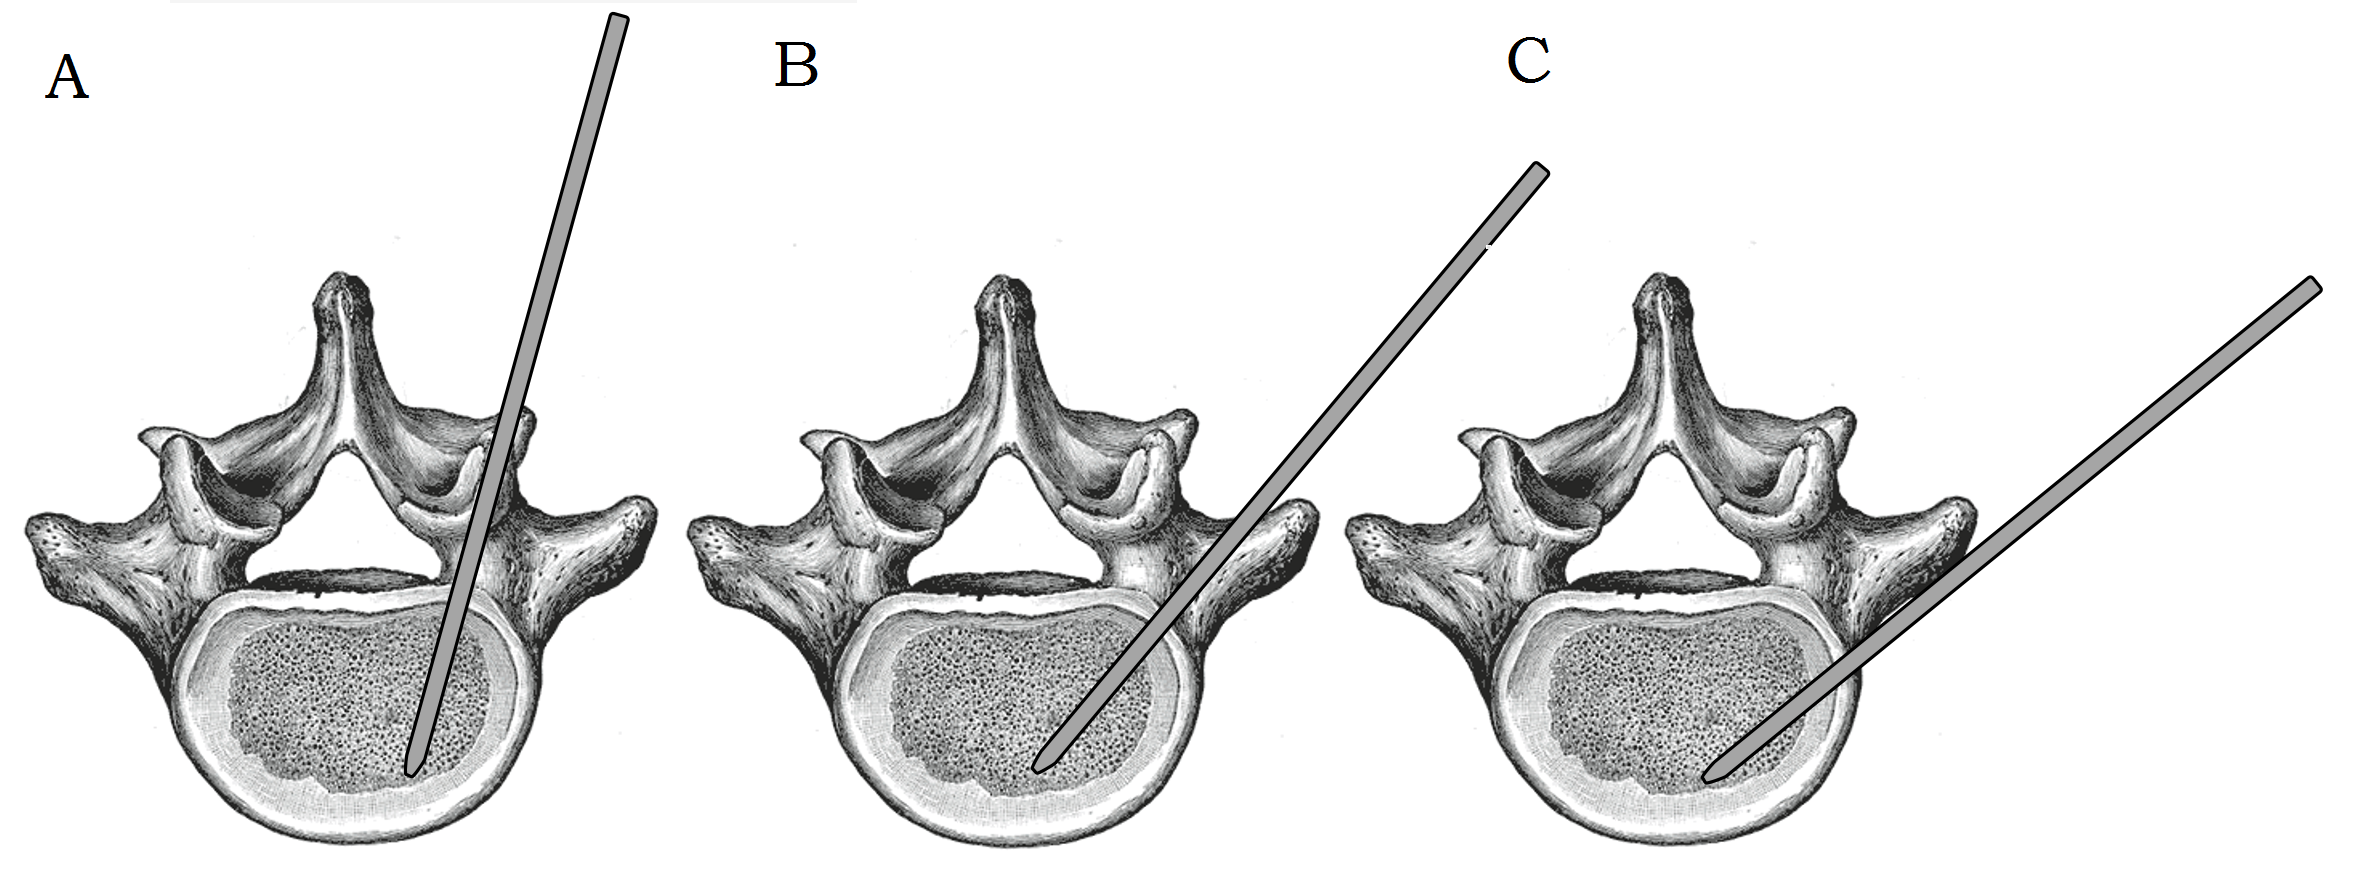
\includegraphics[width=14cm]{images/Vertebroplasty_approach.png}
  \caption{Three approaches to vertebroplasty. A, transpedicular approach, B,
parapedicular approach, C, oblique approach. Adapted from \cite{Gray1918}.}
\label{fig:vpapproach}
\end{figure}



The parapedicular approach involves the needle being inserted transversly across the pedicle until the
vertebral body wall is reached. It has the advantages of allowing the
needle to be positioned ideally for injection, removing the need for
multiple injections to evenly distribute the cement. Although allowing
ideal positioning of the needle tip, it requires the needle to pass
close to the basilar vein, therefore increasing risk of puncturing the
vein.

Finally, the oblique approach avoids the pedicle entirely, entering the
vertebral body in the posterolateral corner and is often used in the
thoracic region where the needle can pass over the top of the rib into
the vertebral body. Disadvantages of this approach include difficulties
in positioning due to the longer needle required and due to the
positioning any extravasation at the needle entry point will be around
the exiting nerve root \cite{pope2014musculoskeletal}.


\begin{table}[hbt]
    \caption{Two randomised clinical trials, with their similar inclusion and
exclusion criteria and results for the study.}
    \label{tab:randclinical}
\begin{tabular}{P{2cm}|P{2cm}|P{2cm}|P{2.5cm}|P{2.5cm}|P{2.3cm}}
Study Author & Number of patients & Type of pathologies & Inclusion Criteria & Exclusion Criteria & Results for osteoporotic patients\\ 
\hline
\hline
Buchbinder et al. \cite{Buchbinder2009} & 71 patients, 35 in VP group, 36 in
placebo group & Vertebral
compression fractures & Pain \textless{} 12 months
duration and presence of one or two vertebral fractures & \textgreater{}
90 \% collapse, presence of spinal cancer, retropulsion of fragments,
hip fracture or infection & No beneficial effect of vertebroplasty over
a sham procedure at 1 week or at 1, 3, or 6 months among
patients\\
\hline
Kallmes et al. \cite{Kallmes2009} & 131 patients, 68 VP group and 63 placebo
group
& Vertebral compression fractures & \textgreater{} 50 years of age 1--3
painful, osteoporotic vertebral compression fractures between vertebral
levels T4 and L5. Fracture \textless{} 1 year old & Evidence of
neoplasm, retropulsion of fragments, hip fracture or infection & No
significant difference between groups one month after the procedure on
measures of back pain intensity, functional disability, and quality of
life\tabularnewline

\end{tabular}
\end{table}

\subsubsection{Results of Vertebroplasty and Clinical
Trials}\label{results-of-vertebroplasty-and-clinical-trials}

The pain relief reported following vertebroplasty is currently not fully
understood; theories include effects on the nerve endings, both thermal
and/or chemical, and the general stabilisation of the vertebrae due to
the material properties of the cement which can restore the vertebral material properties
\cite{belkoff2001biomechanics}. The identification of factors that affect
pain relief are
often difficult to spot, especially with the relatively small patient
populations reported in studies, for example the study by Barr et al.
\cite{belkoff2002ex}, with 47 patients was able to find trends showing
patients with
single level fractures responded better to the procedure. However, the
importance of other factors such as degree of kyphosis and compression,
age, gender and fracture location require a much larger population in
order to obtain any statistical significance.

A large systematic review by Hulme et al. \cite{Hulme2006} of 69 clinical
studies achieved contrasting results to the study described above. A
large proportion of patients, 87 \%, had pain relief of some degree out
of 1552 patients from 32 studies. However, the review also found higher
than expected leakage rates, with leakage occurring in 41 \% of
vertebroplasty procedures and frequent new fractures were found above
and below the augmented level. These fractures give an example of the
need for larger, comparative, blinded and randomized clinical trials,
which could determine whether these fractures are a feature of altered
loading, increased patient activity or whether the new fractures would
have occurred regardless of the vertebral augmentation.

The two studies summarised in Table \ref{tab:randclinical} detail blinded
randomised and
controlled studies by Buchbinder et al. \cite{Buchbinder2009} and Kallmes et
al.
\cite{Kallmes2009}. These studies raised questions over the risks and evidence
for
vertebroplasty due to their conclusions that there is no difference
between the vertebroplasty and placebo groups. The near simultaneous
publication of such results caused many to disregard much of the
positive evidence \cite{Muijs2011} for vertebroplasty. However there are some
considerations regarding both of the trials: the inclusion and exclusion
criteria detailed in Table \ref{tab:randclinical} were neither clear nor well
defined,
failing to take results of MRI scans (Kallmes et al. \cite{Kallmes2009}) and
physical examinations (both) into consideration. Such results would link
to accepted indications of bone marrow oedema and pain on palpation
respectively \cite{Jay2013}. In addition to a population bias towards
fractures less than six weeks old, there was no statistical significance
between chronic and sub-chronic patients (due the small numbers),
prohibiting any insight into which subgroups of patients respond best to
vertebroplasty. Additionally, the National Institute For Health And Clinical Excellence guidance document suggests that consideration for receiving the treatment should be after six weeks, due to the severity of pain reducing over that time and many patients being pain free at six weeks post fracture \cite{Nice2013}. The standard deviation for both pain intensity and
Roland--Morris Disability Questionnaire scores were generally high,
especially at one month post-procedure. For example the mean ($\pm$SD) RDQ score in the vertebroplasty group was 12.0$\pm$6.3, as compared with 13.0$\pm$6.4 in the control group. This highlights the need to
understand where this variation originates from and hence which subset
of patients the treatment is better suited to.

\section{Experimental Studies}\label{experimental-studies}

\subsection{Trabecular Structure }\label{trabecular-structure}

The biomechanical properties of the vertebrae are known to rely heavily
on the trabecular structure, especially the compressive strength and
stiffness which relates to the failure behaviour and elastic behaviour
respectively. The compressive strength originates from the architecture
of the load-bearing trabeculae, which is characterised by thick
trabeculae columns or plates oriented vertically and held in place by
much thinner horizontal trabeculae. This internal structure changes with
age; the vertical plates are reduced to columns through bone remodelling
and horizontal supports are often removed \cite{atkinson1967variation},
\cite{parfitt1984age}.
Osteoporosis is often defined by a reduction in the Bone Mineral Density
(BMD) of 2.5 standard deviations below that of a young, healthy member
of the population of the same gender. However, reports of poor
correlations between the BMD and vertebral fracture rates suggest that a
measure of BMD is not sensitive enough to solely determine fracture
risks \cite{Aaron2000}, hence the trabecular architecture must be studied using
more sensitive and specialised tests.

Methods for studying the trabecular structure of the vertebral body
usually involve mechanical testing of the vertebrae, or trabecular bone
samples in conjunction with a study of the bone density. The trabecular
structure and bone architecture in general can be identified through
calculation of the ash density and comparisons of the trabecular
structure through histological and $\mu$CT examination. The following
measurable parameters are usually measured using $\mu$CT and/or histological
images of the trabecular bone: the bone volume fraction (BV/TV),
connectivity density (Conn.D), Structural Model Index (SMI), degree of
anisotropy (DA) and the trabecular separation, number and plate
thickness (Tb.Sp, Tb.N and Tb.Th respectively) and are discussed in
detail in the following papers by Hulme et al. \cite{hulme2007regional} and Mosekilde et al.
\cite{mosekilde1987biomechanical}.

The ash density allows comparison of the densities of bone samples
through the removal of water and soft tissue in addition to a
calculation of the mineral content using an additional measurement of
the dry weight. Bone marrow and other remaining soft tissue (fat) is
often removed prior to incineration using high-pressure water jets and
acetone washes \cite{keller1994predicting}. The dry weight is measured
following drying
using a recommended 100$^\circ$C furnace for an hour
\cite{keller1994predicting}
and
the dry
density (gcm$^{-3}$) is the weight divided by the specimen volume. To ash the
specimens, they are usually placed in a muffle furnace at 650$^\circ$C for
18-24
hours\cite{mosekilde1987biomechanical}, \cite{keller1994predicting}, which
following cooling can
be reweighed. The
mineral content can be calculated through dividing the ash weight by the
dry weight and ash density by dividing the ash weight by the initial
specimen volume. However, with the adoption of $\mu$CT in most studies
regarding trabecular structure, ash density calculations are rarely
used in more recent studies.

Other parameters of bone architecture (BV/TV, Conn.D, SMI, DA, Tb.Th,
Tb.N and Tb.Sp) are usually defined through $\mu$CT scans of the bone and
analysis using accompanying software to the $\mu$CT scanner. The bone volume fraction, BV/TV, usually
quoted as a ratio or percentage, is a measurement of the proportion of
the total volume of interest that is bone tissue. Conn.D indicates the
number of trabecular connections per volume of interest. The SMI
provides a quantification of numbers of different types of trabecular
element, usually on a scale from 0 to 3 (from rods to parallel
plates)\cite{hildebrand1997quantification}. Tb.Sp and Tb.Th are measured in
length and identify the
average separation between trabeculae and the thickness of trabeculae
respectively, while Tb.N quantifies the number of trabeculae per unit
length. Finally, the degree of anisotropy measures the average alignment
of the trabeculae along a specific axis, where a value of one usually
specifies isotropic behaviour and less than one equates to various
degrees of anisotropy\cite{hulme2007regional}.

The region of interest for taking specimens from the vertebral body
depends on the nature of the study. If the study requires the capture of an
average value for the vertebrae, then the largest possible
volume of cancellous bone is required, while avoiding the cortical bone
and areas where the basivertebral vein intersects
\cite{yoganandan2006}.
Other
studies
have included all cancellous bone between the cranial and caudal
endplates and have used subsections of the vertebral body to identify
differences and changes with age to specific regions \cite{hulme2007regional}.

Bone morphology has been shown to vary greatly between different regions
of the vertebrae \cite{hulme2007regional}, \cite{thomsen2002zone} and between
different ages
of
vertebrae \cite{thomsen2002zone}, \cite{ebbesen1999age}. Animal models are
commonly used for
the in
vitro and in vivo biomechanical models of the spine while testing the
performance of various treatments. However, despite providing a basic
understanding of spinal function, the differences in vertebrae at
different levels and the changes that the vertebrae experience with ageing
mean a single species cannot be used to model the entire spine. Hence
many different large mammals have been used, including bovine, ovine,
porcine and cervine vertebrae which have already been characterised in
the literature \cite{wilke1997sheep,kandziora2001comparison,kumar2000anatomy}. These studies
compare the
anatomical
variation in terms of vertebral body width, height and depth, spinal
canal size and pedicle height and width. Studies detailing similar
anatomical properties for human vertebrae also exist, allowing
comparison and assessment of whether a particular animal model is
appropriate \cite{panjabi1991cervical,Manohar1992}. The
anatomical differences found
between
the animal study papers listed above and the human studies show many
differences between all of the parameters, furthering the idea of
multiple animals being used for different studies. The studies suggested
that sheep spines were much larger than humans, with the vertebral body
height being particularly greater \cite{kumar2000anatomy,kandziora2001comparison}, while the
mean
vertebral width and depth of the human spine are greater than that of
all the animals in the studies (with the exception of the upper thoracic
segments in the deer \cite{kumar2000anatomy}). Much of the geometric and structural variation between human and animal vertebrae may be due to the orientation during walking and therefore load differences. Despite this large difference, muscle forces may add additional loads to the vertebrae, reducing the total loading differences.

A study regarding the trabecular composition of bone samples from the
lumbar spine compared: human, dog, pig, cow and sheep and concluded that
care was required when choosing a suitable animal model for a particular
study, due to the large interspecies differences in terms of Bone Mineral Content (BMC),
volumetric BMD (vBMD), height and area and finally fracture stress
\cite{aerssens1998interspecies}. They found that human BMC and vBMD were
significantly lower
when compared to the other animals in the study, aligning with the
greatly reduced fracture stress also reported; the details of this can
be seen in Figure \ref{fig:bmdgraph}. However, the study also reports a
higher fracture
stress in sheep compared to cows, yet similar values for the BMC and
vBMD, with a similar trend also found between pigs (higher BMD) and dogs
(lower BMD). Having similar density properties yet high fracture stress,
aligns with reports of poor correlations between the BMD and vertebral
fracture in the study by Hordon et al\cite{Aaron2000}.



\begin{figure}[hbt]

\centering
  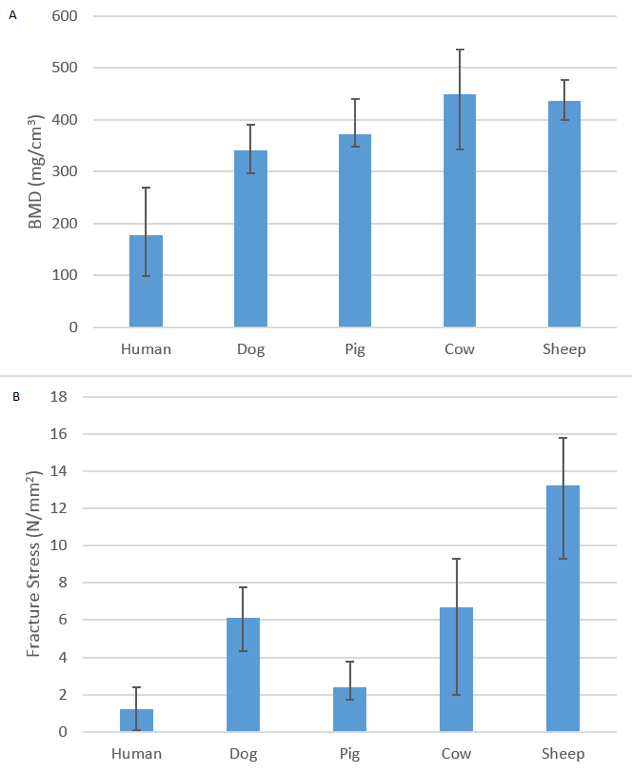
\includegraphics[width=4.21209in,height=5.15601in]{images/bmdGraph.png}
  \caption{A, the mean BMD from
cylindrical cores taken from the lumbar spine of five different species.
B, the mean fracture stress for the same five samples. Bars indicate the
range of values. Adapted from \cite{aerssens1998interspecies}.}
\label{fig:bmdgraph}
\end{figure}

\subsection{Current Studies on Vertebral Fractures and Vertebroplasty
}\label{current-studies-on-vertebral-fractures-and-vertebroplasty}

There have been a considerable number of experimental studies that have investigated the
effects of vertebroplasty through mechanical testing. Often
these studies are carried out in conjunction with computational studies,
where properties are defined experimentally and used to validate
computational models, for example \cite{Wijayathunga2008}. These studies are reviewed in the following section, with a focus on the preparation of
specimens and
methods and with references to notable findings.

\subsubsection{Specimen Preparation }\label{specimen-preparation}

Capturing as much data as possible for a given specimen is vital for understanding
results and allowing those results to be used in many areas of study.
Hence, pre and post-mechanical loading $\mu$CT scans (including
scans before and after cement augmentation) are usually captured.

To simulate physiologic conditions, specimens are often wrapped in
phosphate-buffered-solution (PBS, saline) soaked gauze following
dissection \cite{belkoff2002ex} and are stored at -20$^\circ$C and
thawed for 24
hourssubsubsection
before testing at a non-physiological room temperature\cite{tarsuslugil2013development},
\cite{furtado2007biomechanical}. This difference between room and body temperature may affect the results, whith constituents of the specimens, such as the bone marrow, having different properties at the two temperatures. However, there is a lack of research investigating the effects temperature has on mechanically testing specimens in the literature.
\subsubsection{Mechanical Testing }\label{mechanical-testing}

The generation of vertebral fractures match, in part, the natural
creation of such fractures; compression fractures are usually generated
with an application of force, applied at a low rate, to the vertebrae,
mimicking the gradual creation of fractures in osteoporotic vertebrae
over time, usually in elderly patients. Natural burst fractures are
usually the result of a traumatic event, high energy impacts causing high
rate axial loads through the vertebrae; experimentally burst fractures
are usually generated through dropping a load of known mass onto the
specimen from a calculated height \cite{tarsuslugil2013development},
\cite{wilcox2004dynamic},
generating
comparative forces to a natural traumatic impact. However, other methods
involving biaxial hydraulic testing machines, where high loads (50 --
100 \% of the animals body weight) were applied over a short period of
time, generating the burst fracture \cite{Gurwitz1993}.

Mounting of specimens prior to loading in material testing machines
allows the position of vertebrae to be maintained during testing, whilst
not restricting or confining compression more than necessary. Methods of
mounting allow parallel positioning of the exterior surfaces and allow
perpendicular loading of the vertebrae along the axis. These
requirements for the mounting are usually achieved through potting the
specimens in PMMA \cite{tarsuslugil2013development},
\cite{furtado2007biomechanical}, \cite{ananthakrishnan2005effect}, semi
cured moulding
material \cite{berlemann2002adjacent} or low viscosity resin
\cite{pneumaticos2013effect}.

Methods of loading both a pre-fracture and post fracture/augmentation
rely on mimicking the natural loading of the spine, with similar methods
being used throughout the literature. Loading is carried out with a
materials testing machine, applying loads either under pure axial
compression or allowing flexion of the upper endplate through various
methods. Methods of applying the ``natural'' load include applying the
load or displacement through a steel ball, requiring a specified loading
point and allowing natural motion \cite{tarsuslugil2013development},
\cite{furtado2007biomechanical}.
Applying bilateral
loads through pneumatic cylinders and allowing controlled flexion with
simultaneous compression \cite{ananthakrishnan2005effect} and similarly with
the application of
two anterior and two posterior loads using pneumatic cylinders
positioned so that more of the load was applied to the anterior side
causing flexion \cite{pneumaticos2013effect} were other methods applied in the
literature.
The positioning of the applied load differs in the literature varying
between the mid point of the superior endplate \cite{Barr2000} and one quarter
of the distance of the vertebral body in from the anterior margin of the
superior endplate \cite{belkoff2001biomechanics}.

The definition of the point of fracture varies in the literature, most
commonly the fracture point was defined as the peak on the recorded
load-displacement graph. However, Furtado et al. \cite{furtado2007biomechanical} defined the point of
fracture creation as 75\% of the original vertebral body height, with
the failure strength defined as either the value at the end of the
experiment (75\% of VB height) or the peak on the load-displacement
graph. Pneumaticos et al. \cite{pneumaticos2013effect} defined the point of
fracture (or
maximum fracture load) using the load-displacement graph, where
catastrophic failure could be observed through a sudden jump in the
displacement.

\subsubsection{Results of Mechanical Loading
}\label{results-of-mechanical-loading}

Mechanically loading vertebrae in the study by Furtado et al. \cite{furtado2007biomechanical} showed a
significant correlation between failure strength and the product of BMD
and endplate area, with the range of failure loads being 900 N to 2200 N
for human thoracic vertebrae between T2 and T12. However, the failure
load was defined as the load at a deformation of 75 percent of the
original vertebral height or the peak load before reaching this
deformation, potentially suggesting that the maximum load was not
achieved until after 25 percent strain. This may explain the discrepancy
between these results and those of Pneumaticos et al.
\cite{pneumaticos2013effect} where the
average reported failure load was 6.724 $\pm$ 3.291 kN for intact specimens
using vertebrae between the thoracic levels T2 to T11 from four human
cadaveric spines.

\subsubsection{Experimental Vertebroplasty Compared with Clinical
Vertebroplasty
}\label{experimental-vertebroplasty-compared-with-clinical-vertebroplasty}

Experimentally, transpedicular (uni or bi-pedicular) approaches are more
common in the literature\cite{furtado2007biomechanical},
\cite{ananthakrishnan2005effect}, \cite{pneumaticos2013effect},
although
extrapedicular approaches have also been used \cite{furtado2007biomechanical}.

Although bilateral transpedicular vertebroplasty is the more common clinical
procedure\cite{tohmeh1999biomechanical}, unipedicular vertebroplasty is used
under some
mitigating circumstances often requiring the patient to return for the
second injection. A study comparing bilateral and unilateral
vertebroplasty found no significant difference between the two
procedures in terms of vertebral height and stiffness, possibly
attributed to the central positioning of the cement despite the
unilateral approach \cite{tohmeh1999biomechanical}. The authors reached the
conclusion that a
unipedicular approach is a valid alternative to bipedicular
vertebroplasty and may be especially useful during multilevel
vertebroplasty by reducing the number of injections and hence risk of
cement leaking outside the vertebral walls (extravasation).

\subsubsection{Results following Vertebroplasty
}\label{results-following-vertebroplasty}

\begin{landscape}

\begin{table}[ht!]
\caption{Comparison of the
methods used in studies carrying out vertebroplasty experimentally on
cadaveric specimens.}
\label{tab:vpmethods}
\begin{tabular}{P{2.5cm}|P{5cm}|P{5cm}|P{5cm}|P{5cm}}
Author & Type of specimen & Procedure type \& fill volume & Cement Type
& Key Finding\\
\hline
\hline
Belkoff et al. \cite{belkoff2000biomechanical} & Five vertebral bodies (L1--L5)
from four female cadaveric spines (age, 80 $\pm$ 5 years) &
Transpedicular, 6 ml
fill volume throughout & A bioactive cement, Orthocomp (Orthovita, Malvern,
PA) \& a PMMA based cement, Simplex P (Howmedica, Rutherford, NJ) &
Significantly greater strength following injection of cement, compared
to the intact vertebrae \\
\hline
Furtado et al. \cite{furtado2007biomechanical} & Twenty-six single vertebrae
from 2 female
cadavers (age, 88 and 89 years) & Extrapedicular into anterior third of
vertebral body, 20 \% volume fill, based on height x endplate surface
area & PMMA with 20 \% by dry weight of barium sulfate & Increased
failure strength by a factor of 1.72 post vertebroplasty compared to the
intact vertebrae \\
\hline
Higgins et al. \cite{Higgins2007a} & Human cadaveric, 61 vertebrae from 5
cadavers
with mean age of 81 years & Unipedicular, 10\% and 20\% cement fill by
volume, with unfilled as controls & PMMA & A statistically significant
36\% strength increase as compared with the unfilled controls regardless
of density levels \\
\hline
Pneumaticos et al. \cite{pneumaticos2013effect} & 40 vertebrae from four human
cadaveric
thoracic spines (age range 65-69 years) & Transpedicular, 6 ml fill
volume throughout & PMMA, with 5 to 1 ration of barium sulphate & A
reduced failure load post vertebroplasty, although
non-significant \\

\end{tabular}
\end{table}

\end{landscape}

The methods used to recreate the vertebroplasty procedure experimentally
vary considerably between studies, especially given the sensitivity that
certain studies suggest factors such as fill volume have on outcomes.
Table \ref{tab:vpmethods} shows the methods and some of the more important
variables used
in a selection of studies carrying out vertebroplasty on cadaveric
specimens. Below is discussion of some of the finer points of the
studies, including comparisons to clinical studies.

Identifying the effect of vertebroplasty on intact specimens in the
thoracolumbar region, Higgins et al. \cite{Higgins2007a} found the strength was
increased by a statistically significant amount of $\sim$36\% using 20\% fill volume
and that when comparing the strength increases with BMD, it was found
that those vertebrae with a lower BMD showed a more dramatic increase in
the strength. Conversely Graham et al. \cite{Graham2003}, found that highly osteoporotic
vertebrae showed the least improvement compared to intact vertebrae in
terms of strength and stiffness. Higgins found that the upper thoracic
vertebrae failed to show any significant result following augmentation
of both 10 and 20\% compared to the intact controls. Belkoff et al.
\cite{belkoff2000vertebroplasty} suggested that 7.7 mL of cement was required
to restore the
original strength of fractured osteoporotic vertebrae, this corresponded
to $\sim$24\% volume fill in the lumbar vertebrae tested (in a separate study
to what is presented in. When comparing different cements Belkoff
\cite{belkoff2000biomechanical} found that in order to obtain a significant
increase in the
strength 6 mL or approximately a fill of 18\% was required. Similarly,
Lee et al. \cite{lee2002prediction}, found that between 25 and 30 \% volume
fill was
required to restore strength to the intact level for lower thoracic and
lumbar vertebrae in a clinical study. Graham et al.\cite{Graham2003}, required a fill
volume of 24\% (average 7 mL) to achieve statistical significance,
however this did not return the stiffness to the intact level, and only
returned the strength to the intact level in those specimens with the
highest BMD of their group.

An increase in strength following fracture and augmentation is a
desirable outcome especially for osteoporotic vertebrae where
returning the strength to that of the intact vertebrae may not prevent
fractures. Restoring the stiffness however is believed to be responsible
for pain relief due to the internal stabilisation and prevention of
micro motion, providing a more suitable environment for healing. A study
examining the quantity of cement required to restore the strength and
stiffness of osteoporotic vertebrae having undergone a compression
fracture found that as little as 2 mL of cement is enough to restore the
strength of the vertebrae to the intact value, with the quantity
required to restore the stiffness being between 4 mL and 6 mL depending
on the level (lumbar vertebrae requiring more
cement)\cite{belkoff2001biomechanics}.

Regarding extravasated cement during the vertebroplasty procedure,
Higgins et al. \cite{Higgins2007a} found that an increase in the BMD greatly
increased the tendency for cement to leak, however, this typically was from
the anterior wall of the vertebral (more favourable than into the spinal canal) and was independent of vertebral
level.

Despite previous studies suggesting BMD alone could not be used as an
indicator for vertebral fracture \cite{Aaron2000}, Higgins et al. concluded
that
it was one of the most important factors, conceding however that the BMD
measured ex-vivo is not directly comparable to that measured in a
clinical setting. This was due to differences in the BMD calculation due to the surrounding soft tissue for the \textit{in vivo} scans.

The results from Furtado et al. \cite{furtado2007biomechanical} using an
extrapedicular
vertebroplasty approach achieved approximately 25 \% fill for specimens
which had previously undergone loading to generate a compression
fracture, equating to an average volume of cement of approximately 4.5 ml.
This
augmentation caused a significant increase in the failure load, a factor
of 1.72 increasing the average failure load from 1.61 kN $\pm$ 0.49 kN to
2.63 kN $\pm$ 0.85 kN. A similar result was achieved by Tohmeh et al.
\cite{tohmeh1999biomechanical}, showing that the post augmentation strength is
significantly
higher than the fractured and intact vertebrae. Pneumaticos et al.
\cite{pneumaticos2013effect} found no significant difference between intact and
post
augmentation intact vertebrae, with an average failure load of 5.77 $\pm$
2.13 kN for the augmented intact specimens with 6 mL of cement
injected.

\section{Finite Element Modelling
(FE)}\label{finite-element-modelling-fe}

The use of finite element models of the spine, spinal segments and
vertebrae has been rising rapidly over the past decades. They are being
used to model a range of interventions and devices along with being used
to aid our understanding of spinal biomechanics. The main benefit of
such studies is the ability to test a range of variables and properties
for the same model or specimen, with an additional benefit of assessing
parameters that cannot easily be measured experimentally, such as stress and
strain fields.

Important factors for the generation of biomechanical finite element
models have been discussed previously \cite{Jones2008}--\cite{Viceconti2005}
and include
verification, sensitivity testing and validation of models created. The
first of these factors is an assessment of the numerical accuracy of
the model; given that most studies use commercially available software
for FEA this verification has usually already been carried out, with
documentation available. Additional verification can be carried out
regarding mesh sensitivity and convergence, where the level of detail of
the model is investigated with considerations of accuracy and
computational cost. Sensitivity testing determines the sensitivity of a
model to various input variables and the errors that these input
variables have on the system. Such tests may include the response of the
system to various boundary conditions and material properties.
Validation of models is a proof that the computational results agree
with either \emph{in vitro} or \emph{in vivo} results, however, proof
that the results agree with the \emph{in vitro} model do not mean that
the model is a valid representation of the \emph{in vivo} scenario.

Due to the importance of trabecular bone in many aspects of bone and
spinal research, the methods used to model it are quite detailed
throughout the literature. There are currently two dominant approaches
to modelling trabecular bone using FEA, discussed in detail by Mengoni
et al. \cite{Mengoni2014}. These are $\mu$-FE, which expresses the micro
structure
of
the bone explicitly, and continuum level FE models which represent the
trabecular structure through a continuous model using an inhomogeneous
material property to represent the micro-structure. However, due to the
increased computational cost of $\mu$-FE models, especially for full sized
vertebrae and larger functional spinal units, many current studies use
continuum level FEA, or a variation of, despite the reduced level of
detail.

The studies summarised in Table \ref{tab:geoNmesh} use various methods to
acquire
vertebrae geometry, generate models and apply appropriate material
properties, either from combinations of scan data and experimental data,
or homogenous experimentally defined properties. The variations between
methods and results which can be drawn from these studies is described
below.

\subsection{Geometry \& Meshing}\label{geometry-meshing}

With the growing availability of $\mu$CT scanners and the increasing
resolution available with them, studies using \emph{in vitro}
measurements and handcrafted geometries such as the study by Higgins et
al. \cite{Higgins2007a} in 2007 are being replaced with geometries developed
from
$\mu$CT data. One of the more common methods of generating specimen specific
models of vertebrae is the conversion of voxels from down-sampled $\mu$CT
images into hexahedral elements. The direct conversion of voxels into
elements has the advantage of increasing the simplicity of model
generation, however, this requires real specimens (in the form of animal or human tissue)
which can be difficult to acquire and scan.

\begin{landscape}

\begin{longtable}{P{3cm}|P{2.5cm}|P{5.5cm}|P{5cm}}
\caption{The geometry generation, meshing and material property
assignment methods for 7 studies modelling single vertebrae to acquire
stiffness and strength data.}
\label{tab:geoNmesh}
\\
Author & Geometry Generation & Meshing & Material Properties \\
\hline
\hline
Brown et al. (2014) \cite{RobsonBrown2014} & Used $\mu$CT with resolution of 0.074 x
0.074 x 0.074 mm & Using ScanIP software, segmented CT images down sampled to 1
x 1 x 1 mm and meshed in ScanFE using hexahedral elements and
tetrahedral elements for the smooth vertebral surface & Material
properties assigned using density values from $\mu$CT. No division between
cortical and cancellous bone. Relationship between elastic modulus and
BV/TV value investigated\\
 \hline
 Buckley et al. (2006) \cite{Buckley2006} & Used $\mu$CT data with resolution of 1 x 1
$\times$
1 mm &
Conversion of voxels to hexahedral elements of size 1 x 1 x 1 mm &
Material properties assigned using density values from $\mu$CT. No division
between cortical and cancellous bone\\
\hline
Chevalier et al. (2009) \cite{Chevalier2009} & Used HR-pQCT data with resolution of
0.082 x
0.082 x 0.082 mm & Used $\mu$CT data to find cortical wall thickness.
Surface meshes defined through local triangulation for each cell for the
surface and interior cortical wall boundary. Trabecular bone modelled
with hexahedrons of size 1.312 x 1.312 x 1.312 mm using GMSH software &
Elastic and yield properties assigned to each trabecular element from
$\mu$CT density data\\
\hline
Eswaren et al. (2007) \cite{Eswaran2007} & Used $\mu$CT data with resolution of 0.03 x
0.03 x
0.03 mm & Conversion of voxels to hexahedral elements of size 0.06 x
0.06 x 0.06 mm. 8 node hexahedral elements using in-house software.
Endplates and cortical shell modelled with higher definition using
thickness from $\mu$CT Bone within 180 $\mu$m of the outer structure was
identified as belonging to the cortical shell. & Used a constant
material property for entire model\\
\hline
Higgins et al. (2007) \cite{Higgins2007a} & Taken from in vitro measurements of L1
vertebrae, using flat endplates and curved side walls & Composed of 12
node brick elements using in-house code. Used separate mesh for cortical
walls and different thicknesses for the endplates and posterior and
anterior cortical shell. & Anisotropic through model, using different
material properties for cortical shell, endplates and vertebral
body.\\
\hline
Kinzl et al. (2012) \cite{Kinzl2012} & Used $\mu$CT with resolution of 0.082 x 0.082 x
0.082 mm & Used $\mu$CT data to find cortical wall thickness. Surface meshes
defined through local triangulation for each cell for the outer and
interior cortical wall boundary, meshed using pentahedrals. Trabecular
bone modelled with tetrahedrals & Material Mapping based on porosity
(density). Uses parameters for elastic, plastic and damage behaviour.
Uses elasto-plastic material for the cement augmented
region\\
\hline
Wijayathunga et al. (2008) \cite{Wijayathunga2008} & Taken from $\mu$CT data with
resolution 0.074
x 0.074 x 0.074 mm & Hexahedral and tetrahedral elements using ScanFE
software, smoothing is applied to vertebral surface to improve geometry
& Material properties assigned using density values from $\mu$CT. No
division between cortical and cancellous bone\\


\end{longtable}

\end{landscape}

The cortical surfaces of these models are often rough when just using
voxel to element meshing, for example the models created by Buckley et
al. \cite{Buckley2006} in Figure \ref{fig:buckleymesh}. However, many
studies
introduce
smoothing
to
the surface of a vertebra model. The error introduced from possible
stress raisers when omitting smoothing from the model was questioned by
Chevalier et al. \cite{Chevalier2009}. This study suggested that smoothing, in
the
form of surface meshes representing the cortical walls, successfully
removed the stress raisers and artificial damage zones from their
models. The studies by the group that produced the Chevalier et al. and
Kinzl et al. papers in Table \ref{tab:geoNmesh} use methods for fitting
the vertebrae
surface of the model to that of the scanned specimen, rather than simply
smoothing the voxel to element mesh. Kinzl et al. \cite{Kinzl2012} used a
``marching tetrahedral'' method to extract the surface of the scanned
vertebrae from Treece et al. \cite{Treece1999}, which uses an adaption of the
popular marching cubes method to obtain an iso-surface from discretised
three-dimensional data (from $\mu$CT data).

\begin{figure}[ht!]

\centering
  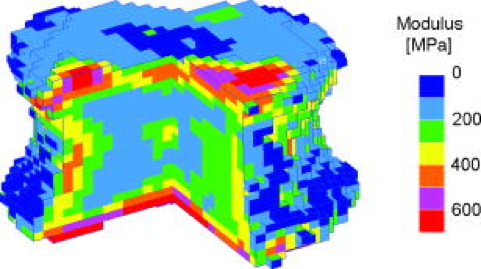
\includegraphics[width=3.20764in,height=1.79236in]{images/voxelFEMesh.png}
  \caption{Voxel finite element mesh of L2 vertebrae used by Buckley et
al. with voxel size of 2 mm \cite{Buckley2006}.}
\label{fig:buckleymesh}
\end{figure}


There is a reduced difference between the structure of the cortical shell and the
cancellous bone structure of the vertebra when compared to other human
bones \cite{Eswaran2005}. Despite this, the cortical walls have been shown to
share a significant quantity of the load, especially in the axial
midsection, where the cross section is narrowest and the load carried by
the cortical wall is greatest \cite{Eswaran2005}. An understanding and correct
modelling of the load sharing between the cortical wall and trabecular
bone becomes more important when considering the variation of the
cortical wall with age, location, level and osteoporotic nature of the
vertebrae in question \cite{Ritzel1997}. Chevalier et al. \cite{Chevalier2009}
found
that
adding a surface faced cortical shell to their models unloaded the
centre trabecular bone and increased the strength and stiffness values
of their models to that of their experimental results. Approaches that
rely on the $\mu$CT greyscale values to assign material properties to
elements, give additional stiffness to the cortical walls due to the
denser and therefore brighter cortical regions in the $\mu$CT images,
without the need for modelling the regions separately.

The increased resolution of the Eswaran et al. \cite{Eswaran2007} study allowed
for a uniform element size and material assignment for the cortical
shell and trabecular bone, relying on the resolution to represent the
higher density of bone within this region. In this case, separate meshes
were used for the two bone types (cortical and trabecular) to extract
information about load sharing between them. However, the required use
of a supercomputer to analyse the FE models limits such models being
used within research, especially where large datasets are required to
investigate population variation.

\subsection{Material Properties}\label{material-properties}

Material properties for continuum level FE models are in general derived
from BV/TV data from $\mu$CT greyscale data for each voxel and assigned to
the matching element. These density values are used to derive elastic
modulus values using a conversion equation. Robson Brown et al.
\cite{RobsonBrown2014}
performed an investigation into the effect of a linear or non-linear
relationship between the elastic modulus and BV/TV. However, due to
lower order errors in the form of the tissue modulus and degree of anisotropy, no benefit
was found when using the higher order relationship. A good
agreement was found with the linear relationship in the Robson Brown
et al study when using a similar method in the study by Wijayathunga et
al.\cite{Wijayathunga2008}.

Chevalier et al. \cite{Chevalier2009} and Kinzl et al. \cite{Kinzl2012} used
other
methods
of representing the material properties. In these studies an enhanced
continuum FE model was used where, rather than using the more common
method of converting $\mu$CT voxels directly into hexahedral elements, they
used high-resolution CT images, which included the cortex and used
fabric-elasticity relationships to describe bone morphology. This
deviation away from the more common methods used by others
\cite{RobsonBrown2014},
\cite{Wijayathunga2008}, potentially allows $\mu$CT at lower resolutions to be
used, which
both reduces computational cost and introduces possibilities for the use
of clinically relevant resolutions. The use of lower resolutions was achieved by using 82 $\mu$m scans and coarsening them to 1.312 mm to mimic common clinical CT
scans. With a focus on identifying modelling errors, a study by Pahr and
Zysset \cite{Pahr2009} compared this enhanced continuum FE models with
standard methods. This study looked at both the effect of smooth cortex
modelling (also used by Chevalier and Kinzl) and the
morphology-elasticity relationship. Pahr and Zysset concluded that this
method of modelling provided statistically equivalent results for the
stiffness of two different models when compared to the more common
method, whilst analysing the model at least 100 times faster.
This reduction in time to analyse the models was due to the reduced sensitivity to mesh size, meaning
mesh density and therefore number of nodes / elements could be reduced.

\subsection{Modelling Vertebroplasty}

The methods used to model vertebroplasty from a selection of studies are
summarised in Table \ref{tab:modVP}. The variation in geometry
generation can be seen
to vary similarly to studies modelling vertebrae alone, however, in
addition to this, the generation of cement geometry and material
properties is also presented due to the range of methods used.

\begin{figure}[ht!]

\centering
  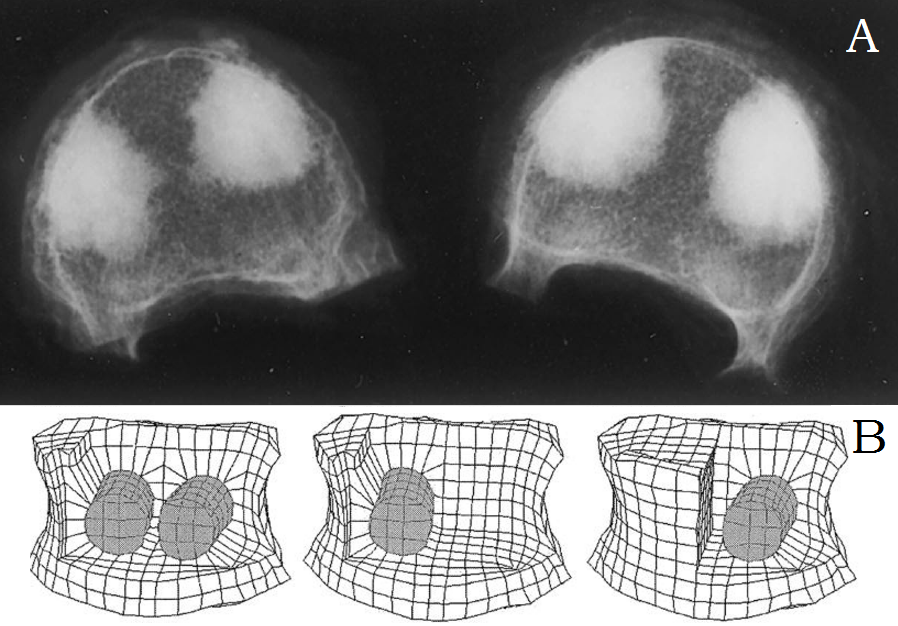
\includegraphics[width=4in]{images/VP_scan_vs_model_lit_rev.png}
  \caption{A: Top view $\mu$CT scans of human vertebrae augmented \textit{in vitro}, showing gradual reduction of cement opacity to the edges of the internal cement volume, adapted from Belkoff et al. \cite{belkoff2001biomechanics}. B: The augmented model generation for the study carried out by Liebschner et al. \cite{Liebschner2001}.}
\label{fig:VP_scan_vs_model_lit_rev}
\end{figure}

Methods of modelling vertebroplasty usually involve using $\mu$CT scans of
augmented vertebrae, masking the internal volume of cement though
greyscale or bone volume fraction. However, the methods used in the
studies by Liebschner et al., Polikeit et al. and Baroud et al.
\cite{Liebschner2001,Baroud2003,Polikeit2003} used approximations of the cement
distribution,
with
the former modelling the distribution according to images from \emph{in
vitro} experiments and clinical trial CT scans, while the other studies
modelled the cement more approximately. Such approximations of the internal volume of cement can be seen in Fig. \ref{fig:VP_scan_vs_model_lit_rev}:B, while $\mu$CT scans in Fig. \ref{fig:VP_scan_vs_model_lit_rev}:A show the much more loosely defined boundaries of the more random internal cement regions. The voxels within the defined
cement region are given linear orthotropic elastic properties described
by a rule of mixture \cite{Chevalier2008}, or more basic material properties
with
constant elastic modulus and Poisson ration \cite{Wijayathunga2008,Liebschner2001,Baroud2003,Polikeit2003}.

\begin{landscape}

\begin{table}[ht!]
\caption{Method of geometry
generation, cement position, location and materials used for five finite
element studies of vertebroplasty.}
\label{tab:modVP}
\begin{tabular}{P{3cm}|P{6cm}|P{6cm}|P{6cm}}

Author & Geometry & Cement position \& shape & Cement
material\tabularnewline
\hline
\hline
Baroud et al. \cite{Baroud2003} & Hand modelled , described in Smit et al.
1997,
two level model & Used 70\% fill of cement & Used previously obtained
values for cement infiltrated bone, 46 times stronger, 12 times stiffer
than surrounding trabecular bone.\\
\hline
Chevalier et al. \cite{Chevalier2008} & $\mu$CT scanned pre and post
augmentation,
model
of vertebroplasty combined cement region with non-augmented scan. &
Cement position and structure taken directly from $\mu$CT scans &
Bone-cement mixture described by a rule of mixture using a tensor for
the isotopic stiffness and for bone stiffness.\\
\hline
Liebschner et al. \cite{Liebschner2001} & Taken from $\mu$CT data & Cement
capsule
design, cylinder with rounded edges. Positioned to investigate
uni/bipedicular vertebroplasty and centred cement positioning. &
Unspecified, PMMA\\
\hline
Polikeit et al. \cite{Polikeit2003} & Taken from CT scans at 1 mm resolution,
manually constructed details not visible. Two level model & Cement
modelled as barrels using radiographs as guides. Positioned to
investigate uni/bipedicular vertebroplasty including one model with 100
\% fill & Constant Young's modulus (3000 MPa) \& Poisson ratio
(0.41)\\
\hline
Wijayathunga et al.\cite{Wijayathunga2008} & $\mu$CT scanned post augmented
vertebrae &
Identified from $\mu$CT scan using constant threshold value based on
greyscale & Used constant properties for Young's modulus and yield
stress. Examined effect of lowering cement modulus to align with that of
cement impregnated bone\tabularnewline
\
\end{tabular}
\end{table}

\end{landscape}

The studies by Chevalier \cite{Chevalier2008} and Wijayathunga
\cite{Wijayathunga2008} were
the
only ones to use experimental cement distributions in their FE
models. The other studies listed in Table \ref{tab:modVP} rely on
previously validated
models of non-augmented vertebrae, with approximately shaped and placed
cement. While such studies can report changes in the overall stiffness,
it is difficult to identify how the load is transferred through the
internal cement and whether it has been modelled with the correct
material properties and boundary conditions for the cement-bone
interface. Wijayathunga et al. \cite{Wijayathunga2008} found large errors
between
experimental and computational augmented vertebral behaviour, concluding
that the representation of the internal cement region as a homogenous
material were possibly inadequate. In light of these results the lack of
a comparison to in vitro results in the Chevalier et al. \cite{Chevalier2008}
study
(in order to study prophylactic vertebroplasty) generates questions of
the accuracy of cement modelling, in both material properties and
boundary conditions.

\subsubsection{Bone-Cement Interface}\label{bone-cement-interface}

The bone-cement interface is an important factor for the vertebroplasty
procedure especially when considering the length of time cement will
remain inside the vertebral body. For this reason and for modelling the
effects of vertebroplasty in general, the bone cement interface needs to
be modelled correctly and accurately.

Zhao et al. and Tozzi, Zhang \& Tong \cite{Zhao2012}, \cite{Tozzi2012}, used a
$\mu$FE
method to investigate the bone-cement interface. They assigned
homogenous and orthotropic elastic-plastic properties respectively along
with examining the effect of friction between the two surfaces
(coefficient of friction 0.3 and 0.4 respectively). Both studies used
stepwise compression testing of their trabecular bone-cement samples
(open cell rigid polyurethane foam, similar to osteoporotic human
trabecular bone and bovine trabecular samples from the iliac crest, Zhao
et al. and Tozzi, Zhang \& Tong respectively) within a $\mu$CT scanner to
assess the evolution of stress in a stepwise fashion. These studies
found good agreement with computational and experimental data, with Zhao
et al. showing that a composite of bone and cement was considerably
lower than what would be expected by cement alone or predicted by a rule
of mixtures, such as that used in other studies described above
\cite{Chevalier2008}. Tozzi, Zhang \& Tong found that greater cement
penetration or
contact area did not increase the compressive strength contradicting the
results of Janssen, Mann \& Verdonschot \cite{Janssen2008} in a FE study of
cemented total hip arthroplasty. This study examined friction
coefficients and morphology under both compression and tension, which
along with the results of Tozzi, Zhang \& Tong potentially suggest that
cement penetration is more important for failure under tension rather
than compressive loading. This advocates the idea of buckling trabeculae
at the boundary of the cement region and a lack of load transfer into
the cement-bone interdigitated region.

In a similar study to those by Zhao et al. and Tozzi, Zhang \& Tong \cite{Zhao2012},
\cite{Tozzi2012}, Kinzl et al. \cite{Kinzl2012a} examined the effect
of PMMA
shrinkage due to polymerisation and different interface properties. The
shrinkage of PMMA upon polymerisation affects the bone-cement interface
due to gaps developing between the two materials caused by the volume
change of the PMMA. Kinzl et al. showed that the shrinkage affected
their models in two ways, firstly, the loss of volume and creation of
gaps reduced the load transmission between the materials and secondly it
created residual stresses in the PMMA, causing bone damage at trabecular
connections from compressive and shear loading.

Sikora \cite{Sikora2013} used FE models generated from $\mu$CT images of ovine
lumbar
vertebra to investigate the bone--cement interface. An analytical model
of the behaviour of trabecular bone struts embedded in cement was used
to impose properties on an interface region defined in the model. The
analytical model was used to predict the interdigitation between the two
materials and forecast the characteristics of failure between them, it
was then used to determine the plastic and elastic properties to apply
to the defined interface mesh. The use of the interface layer with
explicitly defined properties produced a good agreement with the
experimentally determined results for the sample under compression.
However, the study was carried out using cylindrical specimens of height
25 mm and diameter 13 mm, hence a further investigation would be
required to identify whether this method would prove useful for
modelling whole vertebrae.

\subsection{Discussion of FE studies}\label{discussion-of-fe-studies}

Finite element studies modelling vertebrae are currently producing
accurate models for single intact vertebrae. The methods employed by
Chevalier et al. \cite{Chevalier2009} to reduce the need for high resolution
$\mu$CT
scans and instead use more clinically relevant resolution, present a
valuable tool for clinicians. Problems arise however when attentions are
turned to modelling vertebroplasty, specifically, modelling how the two
materials interact while under compression.

Despite the well validated results for the three $\mu$FE interface studies \cite{Zhao2012}, \cite{Tozzi2012}, \cite{Kinzl2012a}, which examined more accurate methods of modelling the boundary between materials, the
computational
cost of
running such simulations on whole vertebrae restricts further research.
Especially given the 700 hours on a high performance computer reported by
Zhao et al. \cite{Zhao2012} for a trabecular sample. Hence, methods employed by
Sikora \cite{Sikora2013} require further testing and validation for whole
vertebrae in order to strike a balance between agreement with
experimental data and computational cost.

\section{Capture of Population Variation}\label{principal-component-analysis-pca}

There is an increasing need for patient variation to be taken into
account in pre-clinical testing; however, experimentally there can be
difficulties in controlling this variation. Obtaining large quantities
of varied tissue can be problematic and time consuming, along with the
problems of characterising the variation. Relating to the spine: in
vitro studies are limited by tissue availability and controlling and
understanding its variability (especially for human studies) and in vivo
studies are heavily limited by the invasiveness of any measuring
methods. Hence, FE studies present a vital method in assessing the
spine. Currently however, the main advantage of FE studies is the
ability to run multiple scenarios for the same model (for example using different material properties for implants or different quantities of cement in vertebroplasty studies); this removes variability from the study. In
order to use FE studies to examine patient variability across the
population then there is a need for large quantities of patient specific
models, similarly to experimental work.

Variability in terms of shape, size and density of vertebrae is high
between individuals, with even greater variability for those with
various pathologies. The effects that this variation has of
vertebroplasty is very important, whether certain variables result in
more positive outcomes or others suggest more conservative treatments
are more suitable. Hence, large sets of models that cover the whole
range of variation across the population and then categorised based of
vertebroplasty effectiveness, could be used to predict outcomes
clinically.

However, these large datasets are difficult to gain access to,
for ethical reasons among others \cite{Grassi2014} and current FE studies
usually
do not attempt to model population variation and instead use vertebrae
specific models from a limited selection of experimental specimens
\cite{Buckley2006, Kinzl2012, Wijayathunga2008, Chevalier2008}. The
alternative to
requiring
cadaveric specimen or clinical scans is to generate large datasets of
vertebral models statistically.

Such statistically generated model studies have been carried out
previously for the femur \cite{Grassi2014, Vaananen2015} and for the
knee joint
\cite{Rao2013, Fitzpatrick2011}. Such studies rely on large databases of
CT scans and
PCA statistical modelling to represent the shape and BMD distribution of bones.

\subsection{Principal Component Analysis Methods}\label{pca-methods}

The purpose of Principal Component Analysis (PCA) is to capture the variation within a given dataset.
It allows an understanding of how different variables interact and what variables control the greatest variation.
Here, there is a focus on using PCA for shape analysis, but the algorithm can be used for many other types of data.
The variation in data is expressed as eigenvalues which become the principal components for the data-set.
These eigenvalues or principal components can then be ranked, allowing an understanding of what variables describe the greatest variation in the data-set (for example the general size or length of a bone).
With regard to the biomedical field, it has been applied to sets of data containing similar shapes, such as sets of human femurs and knee joints.
In these examples it allows an understanding of how the bones vary across the population contained in the given data-set.


Often the first step for PCA is to normalise scaling, rotational and
translation differences between the specimens within the dataset. This
is carried out via generalised Procrustes analysis (GPA) and is often
referred to as a prepossessing step for PCA, it is described in detail
by Grassi et al. \cite{Grassi2014} and V{\"a}{\"a}n{\"a}nen et al. \cite{Vaananen2015}.
Once normalised, matrices are created from columns containing specimens and rows
containing the nodal coordinates for each mesh. Using this matrix and
the mean coordinates from it, the PCA algorithm can be applied, from
which the principal components can be acquired. These principal
components describe each mode of variation, ordered in terms of the
largest variance. To determine how much variation is contained within
each principal component, the eigenvalue for each component can be
divided by the sum of all eigenvalues. The first three modes of shape
variation for a femur (used here as a convenient example) can be seen in Figure \ref{fig:femur}, with the
minimum and
maximum extremes from each mode of variation seen in the wireframe and
shaded model respectively \cite{Grassi2014}.

Similar methods can be used for the BMD and how it varies between
specimens. Once models were generated with BMD assigned to each element,
another matrix is assembled with rows consisting of the BMD of each
element in the mesh. From which a similar method to above can be applied
to acquire the principal components and the amount of variation
contained within each components.

The understanding of the variation of a data-set and its description in terms of a potentially reduced number of components, allows the generation of virtual specimens that fit within the ranges of the input data set.
For example principal components could be altered in terms of their standard deviation about the mean specimen (based on the input data).
This would allow the generation of virtual specimens that fit within the bounds of variation of the current data, but do not currently exist due to possible gaps in the data set.
It also means that the variation can be quantified, allowing effects caused by variation to be studied in an iterative fashion.
For example, in the case of vertebrae, if changes to the diameter of the spinal canal correlate with process length (a correlation that would be difficult to identify without PCA), then the effect this has on specimen strength can be examined in depth by altering the component that controls this relationship.
Models that are described by this relationship and could be generated and solved through FEA, furthering our understanding of the relationship.
However, generating models from the statistical models can produce some problems
regarding reliability. For example, the generated models heavily rely on
the input database, hence the database is required to evenly represent
the entire population. There can also be issues with the generating
algorithm's ability to produce shapes and materials not present in the
starting database \cite{Grassi2014}, \cite{Vaananen2015}.

The Grassi et al. study \cite{Grassi2014} into whether PCA based modelling can
be
used for the femur concluded that such generated models were able to
describe the population of femurs using generated FE models. They found
that 50 modes or the first 50 principal components were required to
accurately reconstruct the femur while maintaining errors below that
originating from pixel size and another 40 to generate accurate density
in the models.

\begin{figure}[hbt]

\centering
  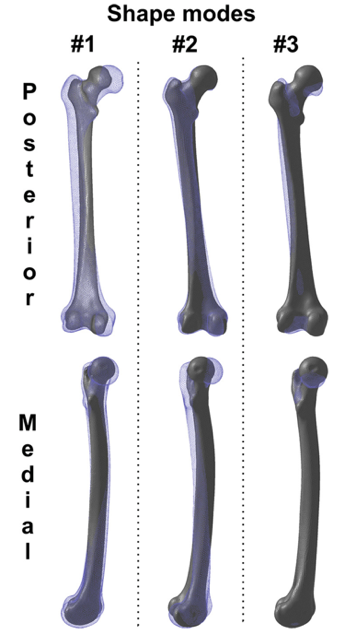
\includegraphics[width=2.30233in,height=4.23373in]{images/femurShape.png}
  \caption{Femoral shape
variations for the first three modes from the PCA. From 115 bones the
maximum eigenvalue is shown with the minimum eigenvalue shown in
wireframe. Taken from \cite{Grassi2014}.}
\label{fig:femur}
\end{figure}


In a study by Fitzpatrick et al. \cite{Fitzpatrick2011} statistical shape
models were
developed in order to identify the relationship between the shape and
function of the palletofemoral joint. Here, 26 magnetic resonance scans
of the knee were taken, from which FE models of the joint in question
were created. PCA was applied to the set of models, from which the first
15 principal components describing the shape were taken, these 15
components accounted for 97.2\% of the total geometric variation, with
the first component (PC1) counting for 47.7 \%. PC1, as is often the
case in biological models, described the variation in the size of the
joint components, with the next two components describing the position
of the patella and details regarding the conformity and depth of the
joint. Following modes of variation described more subtle variations in
the geometry of the model.

In order to assess the robustness or ability to accurately predict
outcomes of the reconstructed bones or joints, the studies
\cite{Grassi2014,Fitzpatrick2011} use a leave-one-out approach. This
approach
neglects one specimen from the development of the shape-function models.
The final model, based on the included specimens can be used to predict
the mechanics or properties of the left out specimen by using the
generated FE models.

\subsection{Discussion}\label{discussion}

The studies described above present useful workflows of generating
virtual subjects from a statistical model acquired from a databases of
scans. Such methods allow a variety of population based studies,
including those regarding the variation of vertebrae across the
population.

The ability to generate models not present in the input dataset and
hence create a large set of models representing the population allows us
to identify relationships not openly visible. For example in the study
by Fitzpatrick et al. \cite{Fitzpatrick2011} a 5 mm change in the patella
position
caused a 25\% increase in the contact pressure mid-flexion. This
relatively easy quantification of the relationship between geometry and
function can easily be transformed to quantify the relationship between
vertebral geometry and the mechanical response to vertebroplasty.
Equally, such relationships could enable the prediction of vertebral
fracture, adjacent level fracture or advise clinicians as to the
quantity and location of cement for different patients.


\section{Conclusion}

Vertebroplasty potentially provides a valuable method to treat patients with osteoporotic compression fractures, however, the uncertainty regarding its effects, especially regarding certain subsets of patients, mean that further research is required. While the mechanisms of pain relief are not fully understood, certain assumptions regarding the mechanical stabilisation and restoration of stiffness can be investigated. Such investigations may help to understand how patient groups respond to the
treatment in different ways.

Current experimental studies have provided a range of useful techniques for mechanically testing vertebrae and for carrying out the vertebroplasty procedure itself. However, obtaining enough vertebrae to represent variation across a population in order understand its effects on different patients is a difficult task and has not been attempted. A possible solution is FE modelling in conjunction with PCA. FE models have been shown to represent the intact vertebrae accurately using both $\mu$FE and continuum level models.

Problems arise when modelling the augmented vertebrae, with few studies modelling specimen specific augmented vertebrae and instead modelling vertebrae with arbitrary volumes of cement. Studies that have modelled and validated against experimental results have shown poor agreement, owing to the incorrect modelling of the cement-bone interface or incorrect selection of material properties for the cement-bone interdigitated region.

Finally, principal component analysis has shown its value in the literature presented above allowing the variation in a set of specimens to be accurately described and in certain cases models have been spawned at standard variations away from the mean.

\section{Aims \& Objectives}

The main aim for the project is to examine whether the outcomes for patients undergoing vertebroplasty are due to underlying biomechanical difference in their vertebrae. To achieve this overall aim three objectives have been defined:
\begin{enumerate}
\item To model specimen specific vertebrae accurately, initially using bovine tail vertebrae and later human vertebrae.
\item To carry out vertebra augmentation experimentally and accurately model the results of this augmentation in specimen specific models. This will require an investigation into the cement-bone interface within FE models, allowing the accurate modelling of augmented vertebrae.
\item To use PCA to identify patient subsets that respond differently to the mechanical outcomes of vertebroplasty.

\end{enumerate}

The first objective will require both experimental and computational work-flows.
Experimental work will focus on testing methods using bovine tail vertebrae, with an aim to adapt methods to use human vertebrae.
Computational work will concentrate on the creation of models of the bovine vertebrae that agree with experimental results for stiffness.

The second objective will involve developing methods of carrying out vertebroplasty on bovine specimens, aiming for clinically relevant volumes of cement using methods similar to those used in a clinical setting.
The computational side to this objective is to further the understanding of modelling cement-bone interfaces, allowing accurate models of augmented vertebrae to be made.

To achieve the final objective, an understanding of PCA will need to be developed along with how to apply it to vertebrae.
This will include methods of registering the volumes that define the vertebral body, applying the PCA algorithm and producing spawned vertebrae to help understand the variation in vertebrae of the population.

\pagebreak

\chapter{Bovine Tail Vertebrae Study}\label{chap_bov}

\section{Experimental Methods}\label{experimental-methods}

\subsection{Introduction}

The experimental methods that have been developed and the early results acquired in this sections allow easier transition to using human tissue  and provide valuable results for the development of specimen specific finite element models. Currently, experimental work is limited to bovine tail vertebrae due to their plentiful nature and relatively similar geometry to human vertebrae. Studying these vertebrae allow the development of methods for material testing, acquiring $\mu$CT scans of the specimens and carrying out vertebroplasty on the specimens. The following section will detail the development of various aspects of the experimental procedure, difficulties encountered and traversed, initial experimental results and finally a discussion of the methods, results and future work.

The steps involved in the developed methods involve dissection of the soft tissue from the vertebrae, potting in PMMA end-caps, scanning using a $\mu$CT scanner, compression testing and augmentation, the order of which can be seen in \cref{fig:exp_flowchart}.
Specimen preparation, fracture generation and initial $\mu$CT scan was undertaken jointly with Ruth Coe (PhD student, University of Leeds). Vertebroplasty (following initial training attempts) and subsequent loading and scanning was carried out solely by the author.

\begin{figure}[ht!]
\centering
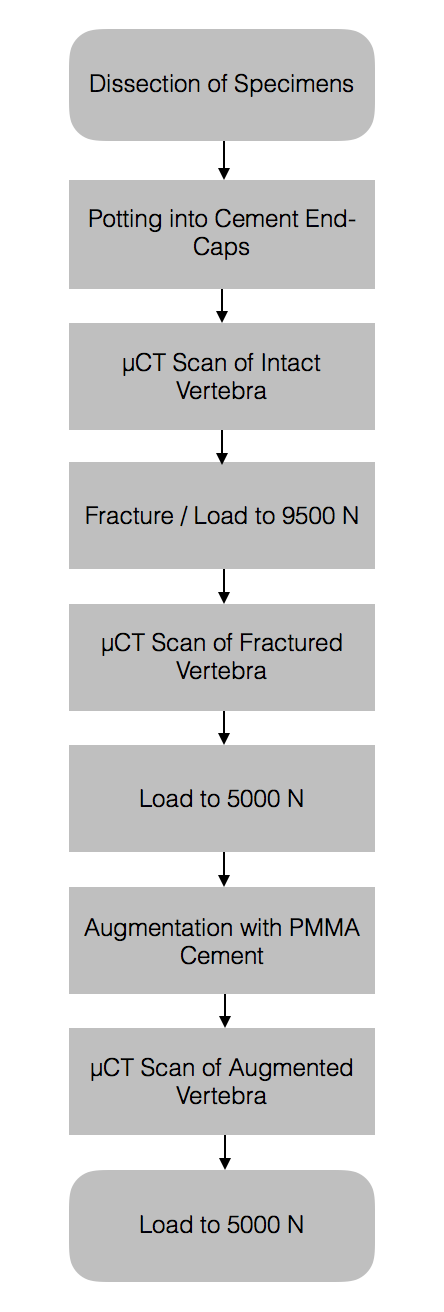
\includegraphics[width=2in]{images/Exp_FlowChart.png}
\caption{Flow-chart detailing the experimental process from initial dissection to final load test.}
\label{fig:exp_flowchart}
\end{figure}

\subsection{Specimen Preparation}\label{specimen-preparation-bov}

Bovine tails were acquired from a local abattoir and frozen to -20$^\circ$C prior to use.
They were defrosted
in a 4\(^\circ\)C fridge for approximately 24 hours before the
initial dissection. The three most caudal vertebral (CC1 to CC3) were kept,
discarding the remainder of the tail due to the elongation of the
vertebral body further distal of the first three vertebrae. In addition
to the elongation of the vertebral body the spinal canal narrows
limiting its ability to house a steel rod used for mounting the vertebrae in PMMA end-caps. Soft tissue was removed from the vertebrae as thoroughly as
possible, including the intervertebral disc material and material
occupying the spinal canal. This was carried out in order to remove
potential error when comparing experimental results of stiffness to the vertebra models developed from $\mu$CT scans (due to
difficulties modelling the soft tissues) and to allow a metal rod through
the spinal canal to aid alignment.


\begin{figure}[ht!]
\centering
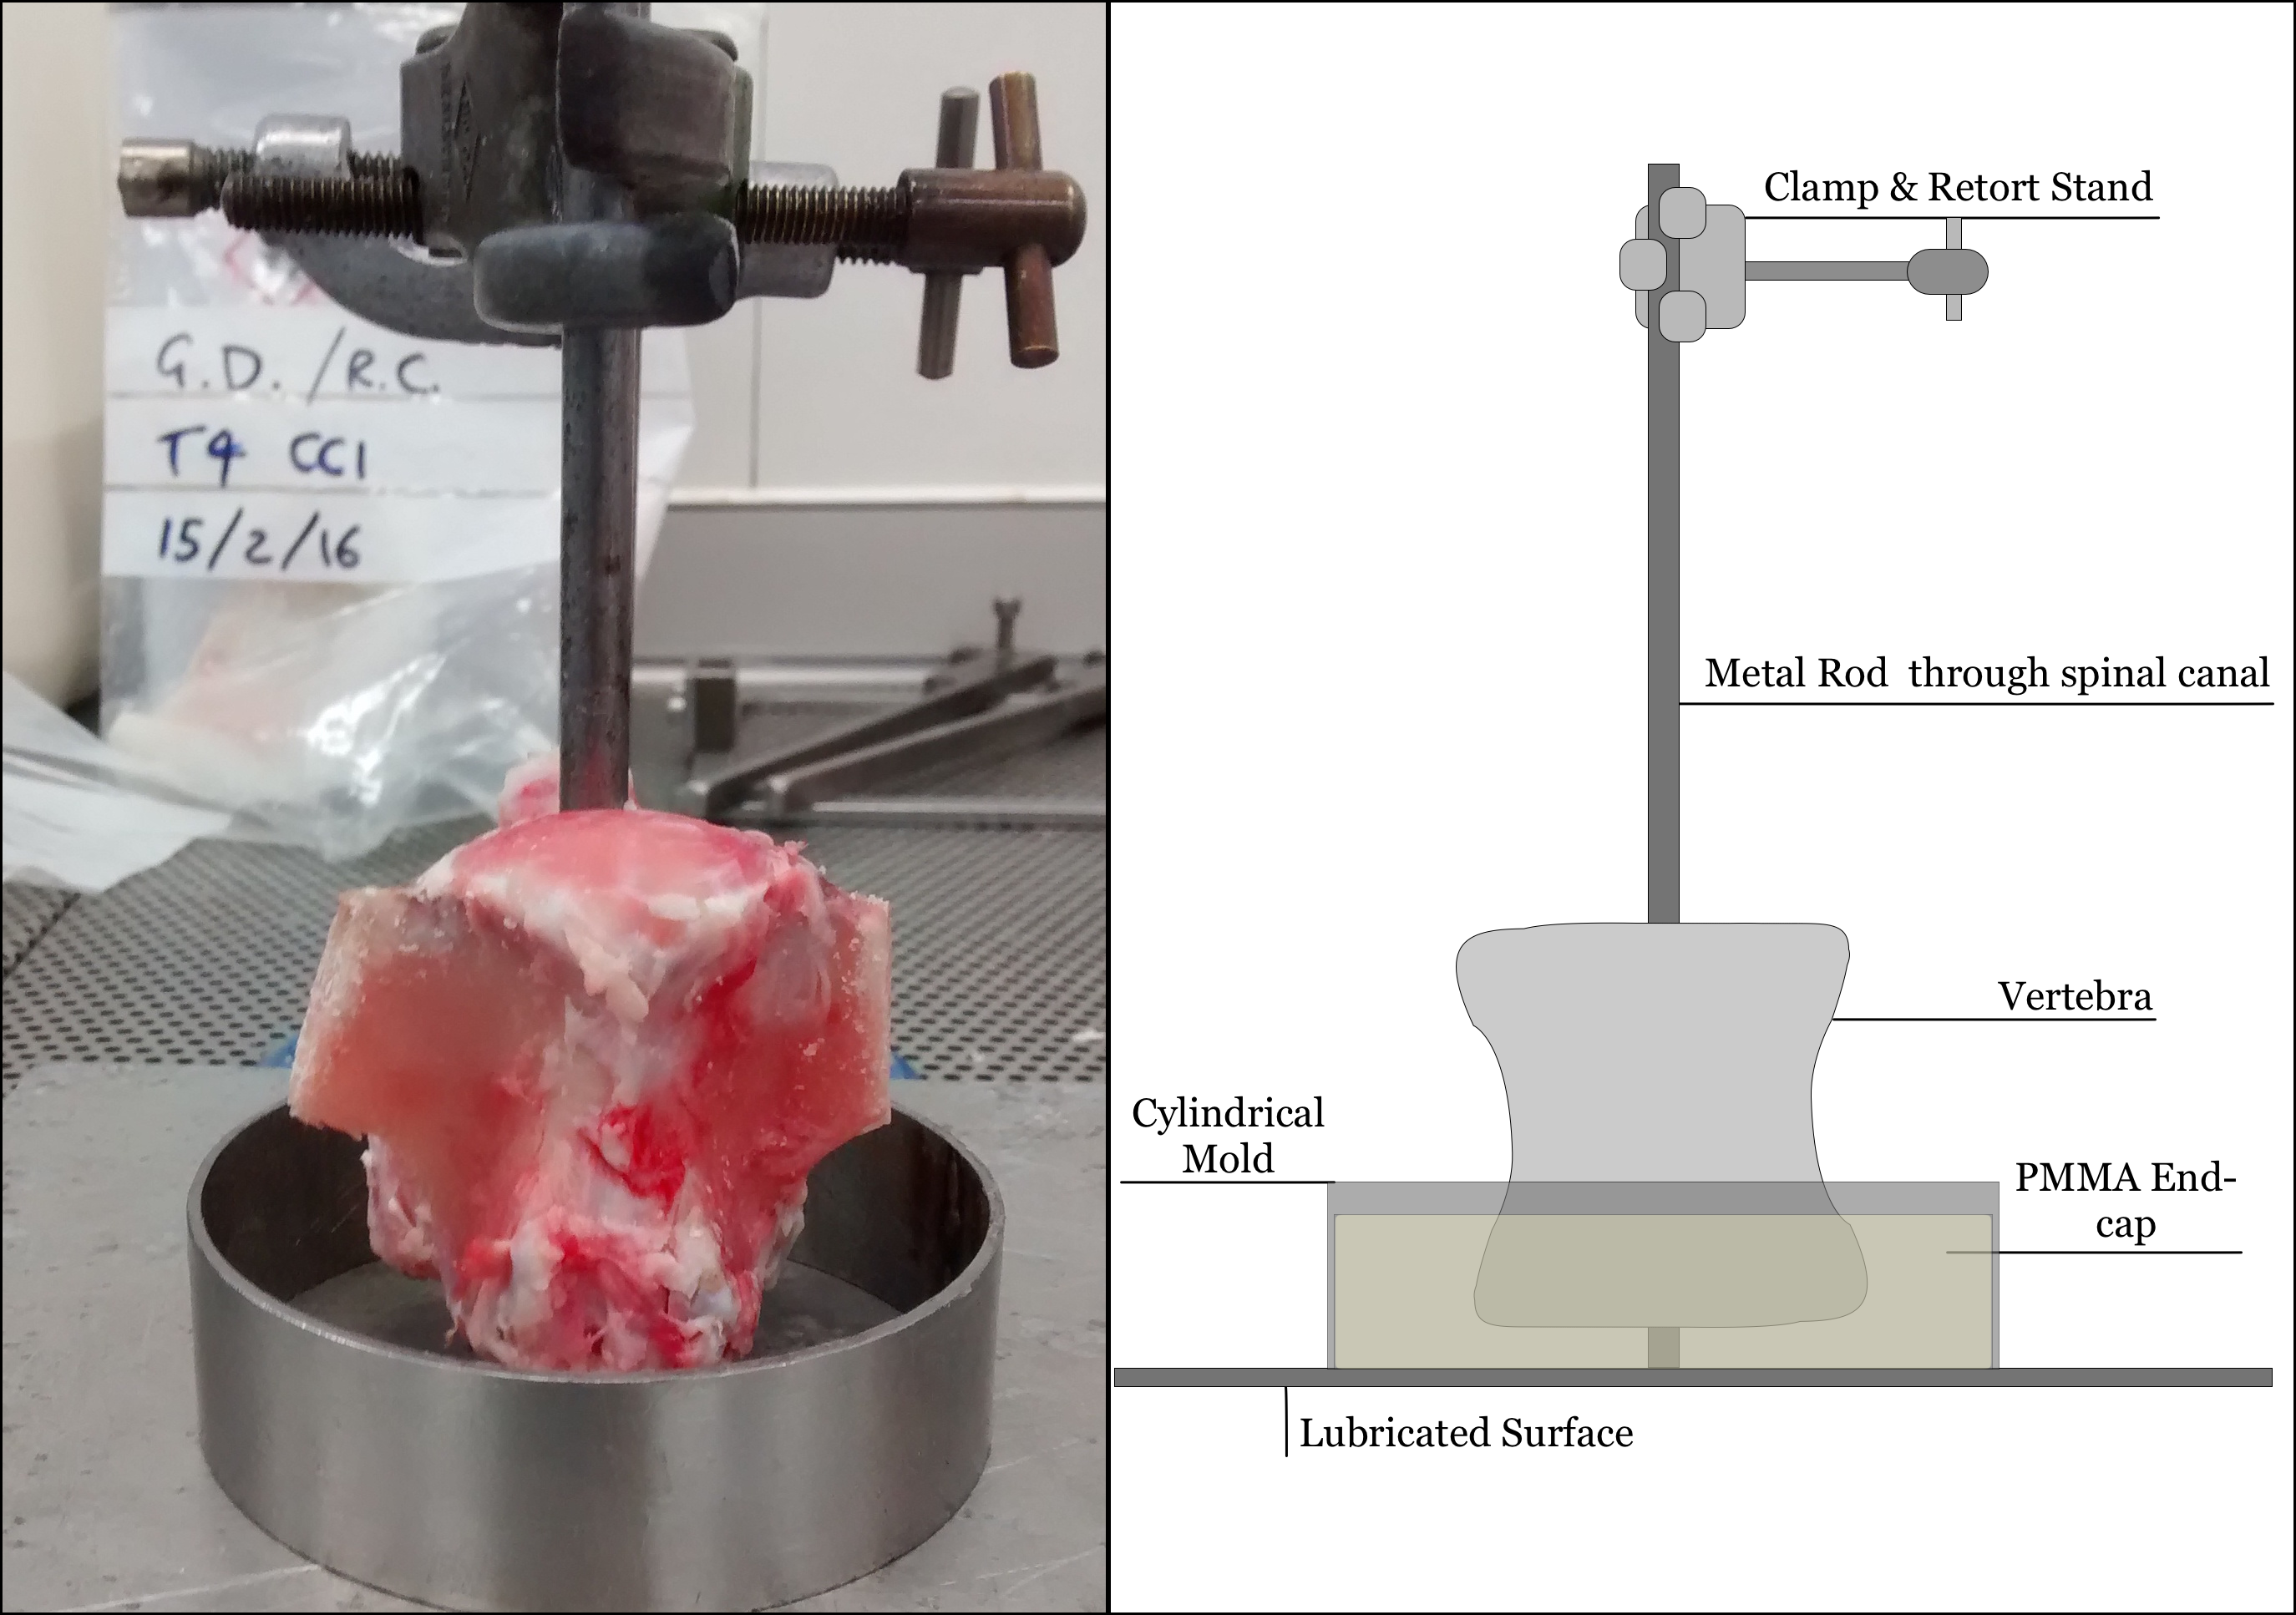
\includegraphics[width=5in]{images/potting_vertebra.png}
\caption{Photograph and diagram depicting the method of creating end-caps for the specimens.}
\label{fig:potting_vertebra}
\end{figure}



Once dissected (and in subsequent breaks between procedure steps) the
vertebrae were wrapped in phosphate buffered solution (PBS) soaked
tissue, in an attempt to limit the vertebrae from drying.
The specimens were potted in PMMA end-caps to allow repeated loading of the vertebrae with
the same orientation and positioning, while constraining the vertebrae
as little as possible and allowing flexion of the upper endplate. The setup for potting the vertebrae can be seen in \cref{fig:potting_vertebra}.
Vertebrae were held using retort stands and clamps holding a rod placed
through the spinal canal. Depending on the level of the vertebrae the
spinal canal was packed with foam around the rod forming a snug fit
while the vertebrae was held approximately 5 mm above a petroleum jelly
lubricated metal surface. Also, depending on the level of the vertebrae,
any pedicles that protruded past the limits of the metal cylinders were
removed with a hacksaw at their base to prevent issues with the loading
and scanning tests which followed, most often this was limited to the
most caudal vertebrae and can be seen in \cref{fig:potting_vertebra}. Lubricated hollow metal cylinders of \(\sim\)10
cm diameter were used to form the endplate when the 2:1 powder to liquid
component PMMA mixture was added. PMMA was added until the endplate of
the vertebral body was covered up to the point where the body becomes
concave. After approximately 20 minutes the PMMA had sufficiently set to turn over
the vertebra and create the end-cap at the other end using the same
process with the addition of a level to ensure the creation of parallel
end-caps.

Once the PMMA was set the vertebrae were wrapped in more PBS soaked
tissue before being frozen or stored in a fridge until the vertebrae
were loaded to fracture. The specimens were frozen only if more than 24 hours
would pass before the next stage of testing to reduce the number of
freeze thaw cycles.

\subsection{Axial Compression}\label{axial-compression}

\subsubsection{Fracture Creation}\label{fracture-creation}

All specimens underwent axial compression using a material testing machine
in order to generate fractures within the vertebral body. Mounted
vertebrae were placed between two steel end-plates, the lower of which
contains four screws to inhibit lateral motion of the specimen when
under load and the upper plate contains similar screws, with the
addition of a chamfered hole. This chamfered hole allows the
alignment of the specimen so that the loading point was directly below
the head of the testing machine using the marker located above the centre of the vertebral body. The steel ball becomes the centre of rotation for
the free to rotate upper end-cap. This permitted rotation mimics natural
loading of the vertebrae and increases the likelihood of physiological
anterior wedge fractures. Details of the setup can be seen in
\cref{fig:expsetup}.

\begin{figure}[ht!]

\centering
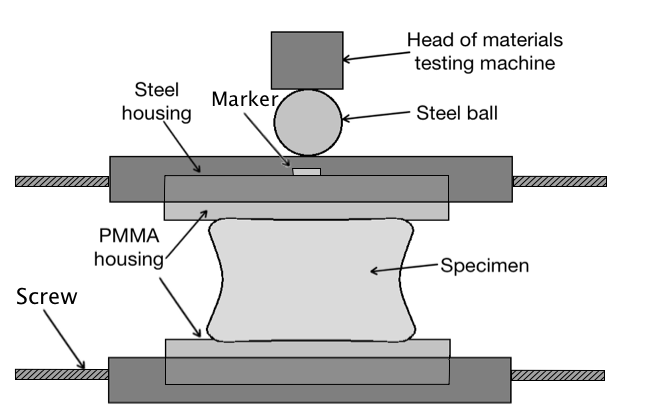
\includegraphics[width=3.68472in]{images/instrom_loading_diag.png}
\caption{The experimental setup for axial loading the vertebral
specimens.}
\label{fig:expsetup}
\end{figure}

Loading of the vertebrae starts with a preload from 50 N to 300 N for
10 cycles at a rate of 1mm/minute to remove any viscoelastic effects of any remaining soft
tissue. Following the preload, displacement was increased by 1 mm/minute
until either the load reached 9500 N (due to the 10 kN load cell limit)
or a visible failure occurred on the real-time load-displacement plot during compression.
This failure was observed as a peak in load with the compression being stopped once
clear decrease in load was observed. Both scenarios can be seen in \cref{fig:failure_non_failure}.



\begin{figure}[ht!]
\centering
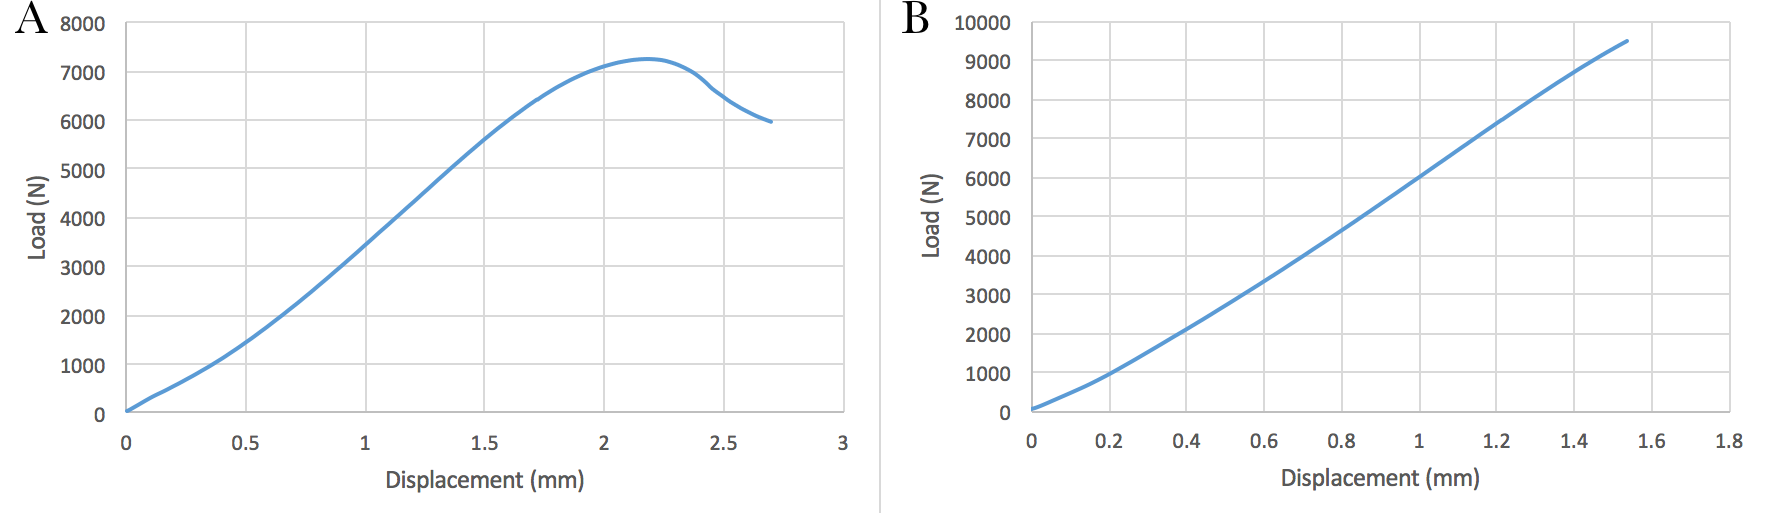
\includegraphics[width=16cm]{images/comparing_failureand_nonfailure.png}
\caption{The difference between failure (A) and non-failure (B) for bovine tail vertebra compressed to a maximum load of 9500 N or until a peak was observed.}
\label{fig:failure_non_failure}
\end{figure}

\subsubsection{Post Fracture \& Post
Augmentation Loading \& Stiffness
Calculation}\label{post-fracture-post-vertebroplasty}

In order to find the stiffness of the previously fractured and augmented
specimens a similar loading procedure was used. However, following the
preload, compression was stopped when the load reached 5000 N as a means
to limit additional damage and fractures to the vertebrae. This ensured that the vertebral stiffness across the three stages (intact,
post-fracture and post-augmentation) was calculated from the same range of loads (0 - 5000 N). To examine the effect that the initial load to failure has on the following loads, both post-fracture and post-augmentation, a control specimen was used. This control (T1 CC3) was only loaded up to 5000 N before ending the test.




%\begin{table}[ht!]
%\centering
%\caption{My caption}
%\label{my-label}
%\begin{tabular}{l|c|c|c}
%         & \multicolumn{3}{c}{Greatest Gradient (N/mm)}          \\ \hline
%Vertebra & \textless 1500 N & \textless 5000 N & \textless 9500 N \\ \hline \hline
%T8 CC1   & 4396.6           & 5914.3           & 6474.7           \\
%T8 CC2   & 7824.0           & 8132.8           & 8378.5           \\
%T8 CC3   & 3526.3           & 5680.6           & 6416.3           \\
%T9 CC1   & 4688.8           & 5833.5           & 6843.1           \\
%T9 CC2   & 3580.2           & 4449.8           & 4950.4           \\
%T9 CC3   & 3539.1           & 5093.7           & 5968.4
%\end{tabular}
%\end{table}

%add link to graph of load-disp showing wonky "linear region"

The stiffness of the specimens throughout their tests was calculated using a
Matlab (Mathworks) script on the raw data from the materials testing machine. The script was adapted from a script written by R. Coe (University of Leeds, 2016). The script
allowed the limits of the range of interest to be set and, using a defined
segment size, incremented over the data reporting the greatest stiffness found
in a segment. The segment size was set to 0.3 mm. The script iterated over the
data in overlapping increments of 0.1 mm and the range of interest was set to 0 - 5000 N, this can be seen in \cref{fig:load_disp_incr}.

\begin{figure}[ht!]

\centering
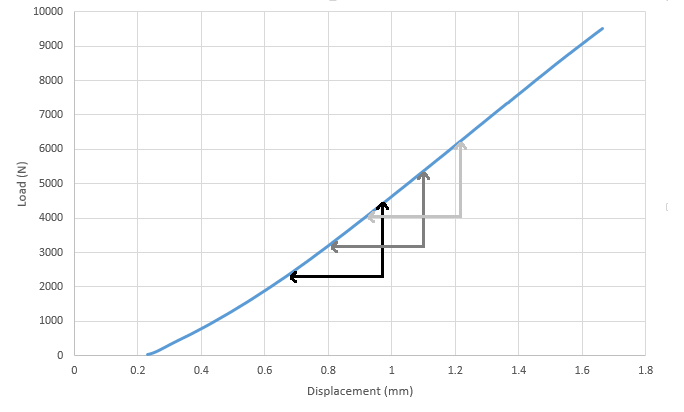
\includegraphics[width=4.18472in]{images/load_disp_incr.png}
\caption{A typical load displacement curve showing how the gradient was taken from 0.3 mm long sections incremented at 0.1 mm across the length of the curve.}
\label{fig:load_disp_incr}
\end{figure}

If the load-displacement curves were perfectly linear within the ``linear region" the stiffness in the three ranges of interest in \cref{fig:barchartcompgrads} would give an equal value for the stiffness or maximum gradient. However, given that these values were found to differ for the three ranges it suggested non-linear behaviour.
 As shown in \cref{fig:barchartcompgrads} the recorded maximum stiffness varies greatly depending on what portion of the load displacement graph was being examined. The average difference between the 0 - 5000 N section and the 0 - 9500 N section was much smaller compared to the 0 - 1500 N section, hence 5000 N was used as the limit on the already fractured vertebrae tests. Due to the slight convergence towards 5000 N, this value was seen as a compromise between the risk of further damage whilst still obtaining a genuine value for the stiffness.


\begin{figure}[ht!]

\centering
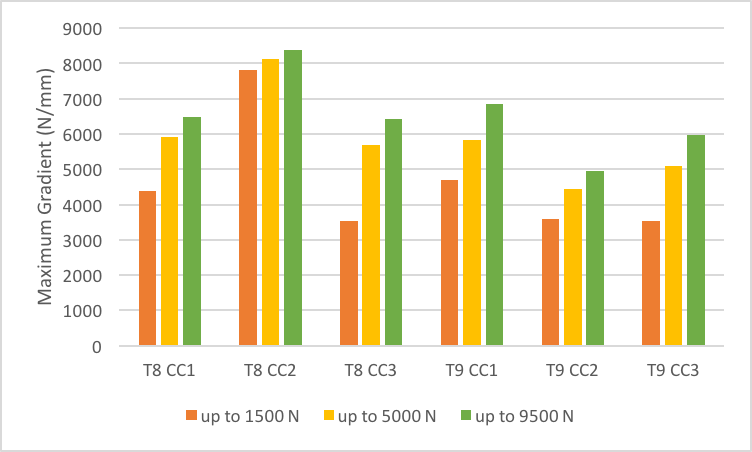
\includegraphics[width=4.18472in]{images/barchartCompGrads.png}
\caption{The difference seen when measuring the greatest gradient (stiffness) using different portions of the load displacement curve. From 0 to 1500 N, 0 to 5000N and 0 to 9500N.}
\label{fig:barchartcompgrads}
\end{figure}


\subsection{Vertebroplasty }\label{vertebroplasty-bov}
The procedure was developed in collaboration with two clinicians (Dr Peter Loughenbury \& Dr Vishal Borse) from the Leeds General Infirmary. Subsequent tests of the procedure were undertaken with the aid of Dr Sebastien Sikora, Dr Fernando Zapata Cornelio \& Ruth Coe (Research Fellow, Research Fellow \& PhD student respectively), while specimens with results presented here were augmented solely by the author.
Due to the differences between human and bovine vertebrae it was not possible to perform bi-pedicular vertebroplasty on the bovine specimens using the methodologies established for human vertebra.
The main difficulty was the greatly increased density of the bovine vertebra bone, meaning that rather than pushing the vertebroplasty needle into the vertebra by hand, a mallet and vice to hold the vertebra were required. In addition to this, the force required to inject cement into the vertebral body was greatly increased.
The vertebroplasty method for bovine tail vertebra was therefore developed over several iterations due to these difficulties. This sub-section details the initial procedure, the problems encountered and solutions developed to allow a clinically relevant volume of cement to be injected and captured in $\mu$CT scans.

\subsubsection{Initial Procedure}

The procedure was initiated by using bone nibblers to remove the rounded end of both posterior pedicles, providing a surface to start the needle entry. While holding the vertebra in a table mounted vice the needle's markings were used to estimate the depth and angle needed to reach the anterior quarter of the vertebral body. The placement of the needle required care to ensure the pedicle was not damaged through splitting as it was inserted. A mallet was used to insert the needle until it was at the depth
required; the procedure was repeated for the other pedicle, reusing the same needle.



The PMMA cement was mixed 1:1 monomer to powder to ensure that it could be drawn up via the syringe and to allow enough time to inject the cement before it thickened and set. This additional setting time and reduced viscosity is also used by clinicians, who use ratios up to 0.74 monomer to powder with no adverse outcomes associated despite the reduced modulus and strength often reported \cite{Belkoff2002,Jasper1999}.
While the vertebra was held in the clamp of a retort stand, the syringe was attached to the needle, which in turn was inserted into one of the pre-made tracks through the pedicle into the vertebral body.
%The syringe was then attached to the needle, with the interior rod removed, which was inserted to one side of the vertebra mounted using a retort stand.
Cement was pushed into the vertebrae using the syringe, until $\sim$3-4 mL was inserted into both sides of the vertebrae, with cement being used to back fill as the needle was removed. The vertebrae were then left for approximately an hour until the cement had set before scanning.

% Add picture and clarify


\subsubsection{Complications and Changes to the Procedure}\label{complications}

Various problems were encountered while carrying out the procedure that required the methods to be adapted. These challenges and their solutions are described below.

\paragraph{Vertebral Temperature}
The first of these was the difficulty found injecting any cement into the vertebra. With the initial specimens, cement was injected but it was mainly reserved to the needle tracks rather than the vertebral body. To counter this the vertebrae were warmed to 37$^\circ$C for an hour or until the internal temperature of the vertebrae had reached this temperature (using a temperature probe in the vertebroplasty needle hole). This meant that the bone marrow inside the vertebrae was no longer solid and therefore could be displaced by the cement making the injection much easier.

\paragraph{Radio-opacity of Cement}
A second problem was the opacity of the cement on $\mu$CT scans, which proved difficult to segment and separate it from the trabeculae in the vertebral body as can be seen in \cref{fig:withWithoutBaSO4}:A. Here, the cement was indistinguishable from the bone marrow and can only be seen in the needle channel. The solution to this was to mix barium sulphate (BaSO$_4$) with the PMMA to achieve the radio opacity seen in \cref{fig:withWithoutBaSO4}:B, where the bright area in the centre of the vertebral body is the injected cement and BaSO$_4$ combined. Due to the hydrophilic nature of the BaSO$_4$ powder it was important to use a completely dry beaker when thoroughly mixing it with the PMMA powder to limit aggregation of the BaSO$_4$, which can be seen in the bright spots in \cref{fig:withWithoutBaSO4}:B. The two components were used in a 1:4 BaSO$_4$ to PMMA powder ratio, mixed 1:1 with the liquid PMMA component.

\begin{figure}[ht!]
\centering
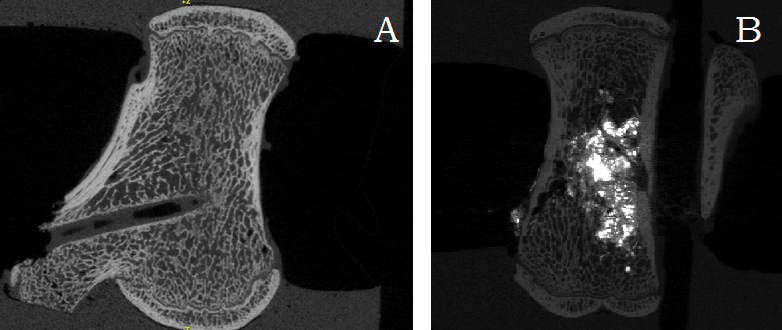
\includegraphics[width=4.18472in]{images/withWithoutBaSo4.png}
\caption{A: $\mu$CT scan of an augmented vertebrae, with some visible PMMA residing in the needle channel. B: $\mu$CT scan of an augmented vertebrae using PMMA mixed with barium sulphate.}
\label{fig:withWithoutBaSO4}
\end{figure}
\paragraph{Cement Leaking from Vascular Channels}
Preventing the cement from exiting the vertebrae from vascular channels while injecting the cement proved to be another obstacle to achieving a physiologic fill volume for the vertebrae. These channels lead both out the anterior face and from the vertebral body into the spinal canal, this can be seen in \cref{fig:cementleakage} and \ref{fig:2vertWithoutBluTac}. In the body these channels would be filled with vasculature preventing the cement leaking through them. Two main methods were used to stop cement leaking while carrying out the procedure on the bovine tail vertebra. The first was to use the same rod used for mounting the vertebrae in their end-caps to limit the passage of cement into the spinal canal. The second was to use blu-tac to cover the external vascular channels, wrapped with cling-film to hold it in place. This allowed any bone marrow free passage out of the vertebrae, but enough resistance to limit the flow of cement.

\begin{figure}[ht!]
\centering
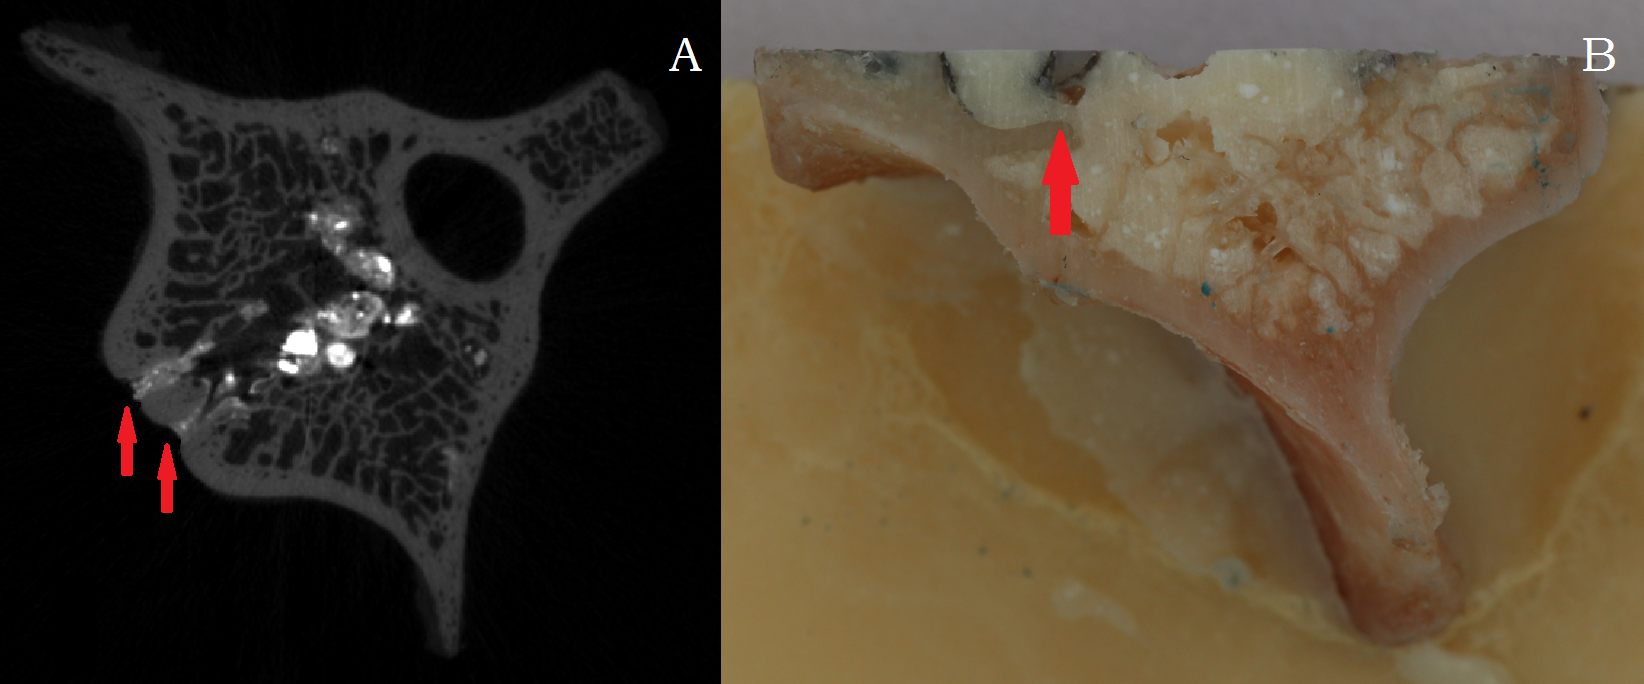
\includegraphics[width=4.18472in]{images/cementleakage.png}
\caption{A: $\mu$CT scan of an augmented vertebrae showing the cement leaking from vascular channels on the anterior side. B: Photograph of an augmented vertebrae cut into four quarters showing a vascular channel leading into the spinal canal.}
\label{fig:cementleakage}
\end{figure}

\begin{figure}[ht!]
\centering
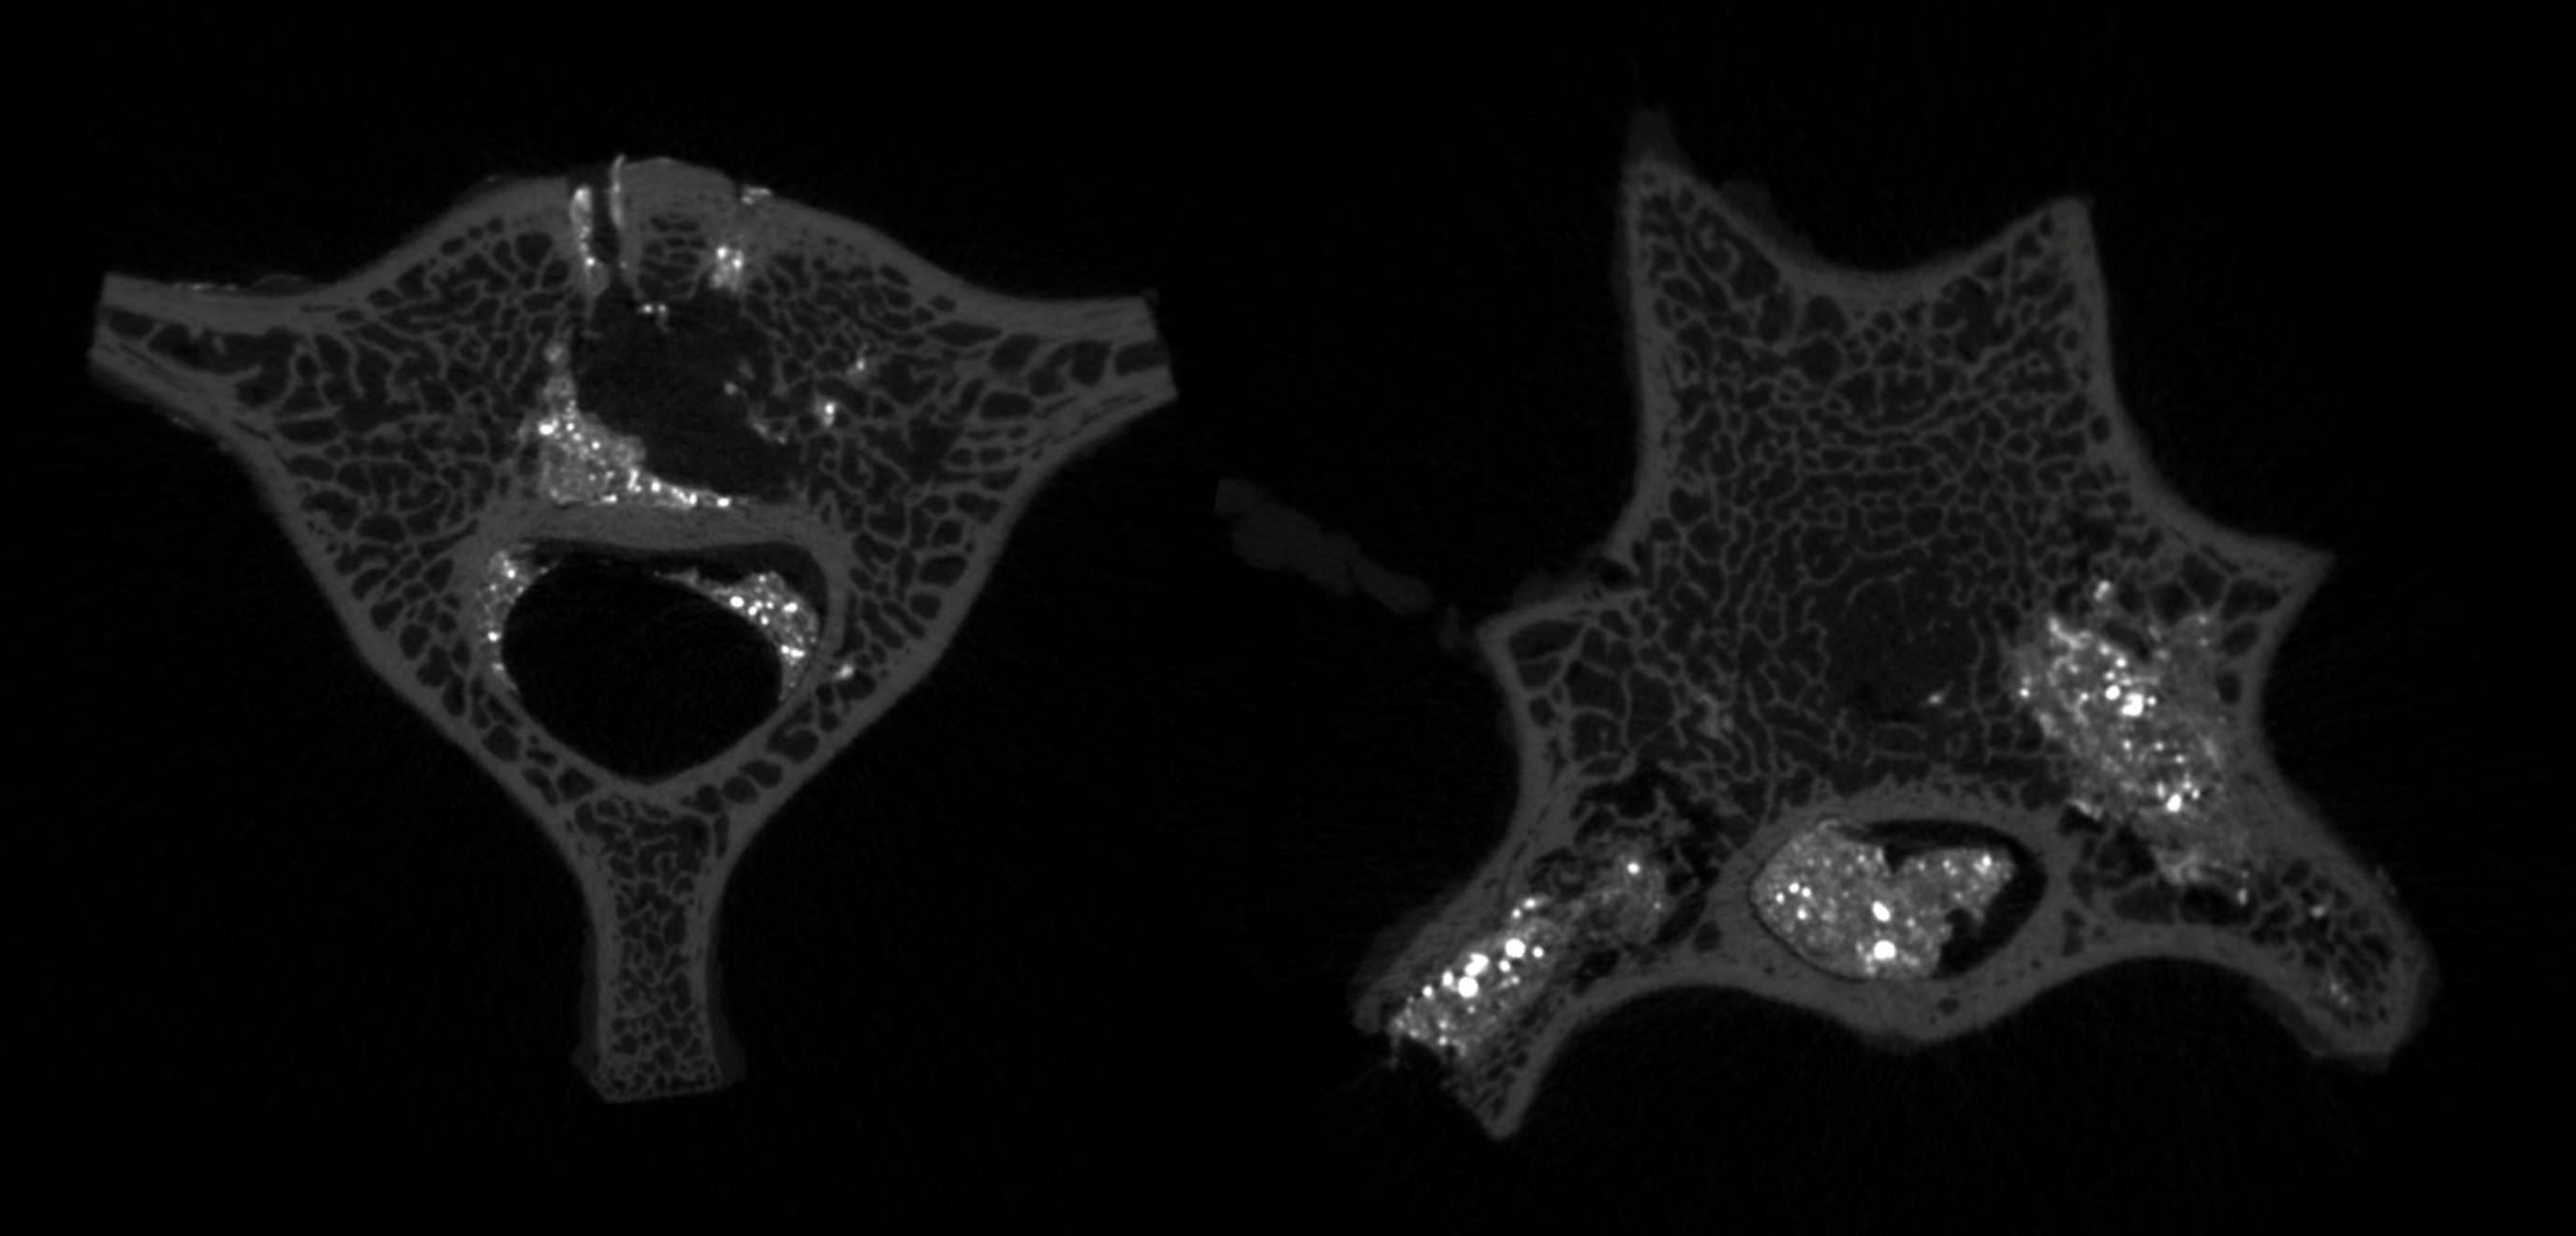
\includegraphics[width=4.18472in]{images/bigLeakage_noBluTac.png}
\caption{$\mu$CT scans of two vertebra, showing the cement leaking into the spinal canal and out of the vascular channels and the vertebral surface.}
\label{fig:2vertWithoutBluTac}
\end{figure}
% add figure of scan to make clear what the right hand pic is


\subsection{MicroCT Scanning}

$\mu$CT scans were taken at three occasions during the experimental process. These scans occur before and after the initial load to failure, then following the augmentation of the specimens. The process requires the vertebrae to be defrosted and at room temperature, given that the radio-opacity of water differs between solid and liquid states, hence vertebrae were usually defrosted overnight in a 4$^\circ$C fridge. Vertebrae were loaded two at a time in a carbon fibre loading cradle designed for the HR-pQCT (XtremeCT, Scanco Medical AG, Switzerland) scanner. The settings used for the scans were: an isotropic voxel size of 82 $\mu$m, energy settings 900 $\mu$A, 60 kVp and 300 ms exposure time.

\subsection{Results}\label{results}

The stiffness values for 12 bovine tail vertebra from the first to third vertebra down, shown in \cref{fig:allexpData}. Of the twelve vertebra only two, the first and second tail vertebra of the second tail (T2 CC1 \& T2 CC2), were fractured. The remaining nine (excluding T1 CC3, the control) reached 9500 N and therefore did not fail. It is also difficult to see whether the initial load to failure had any effect on the subsequent loads. This is mainly due to the lack of control specimens and the large variation of results in general following the first load.

\begin{figure}[ht!]
\centering
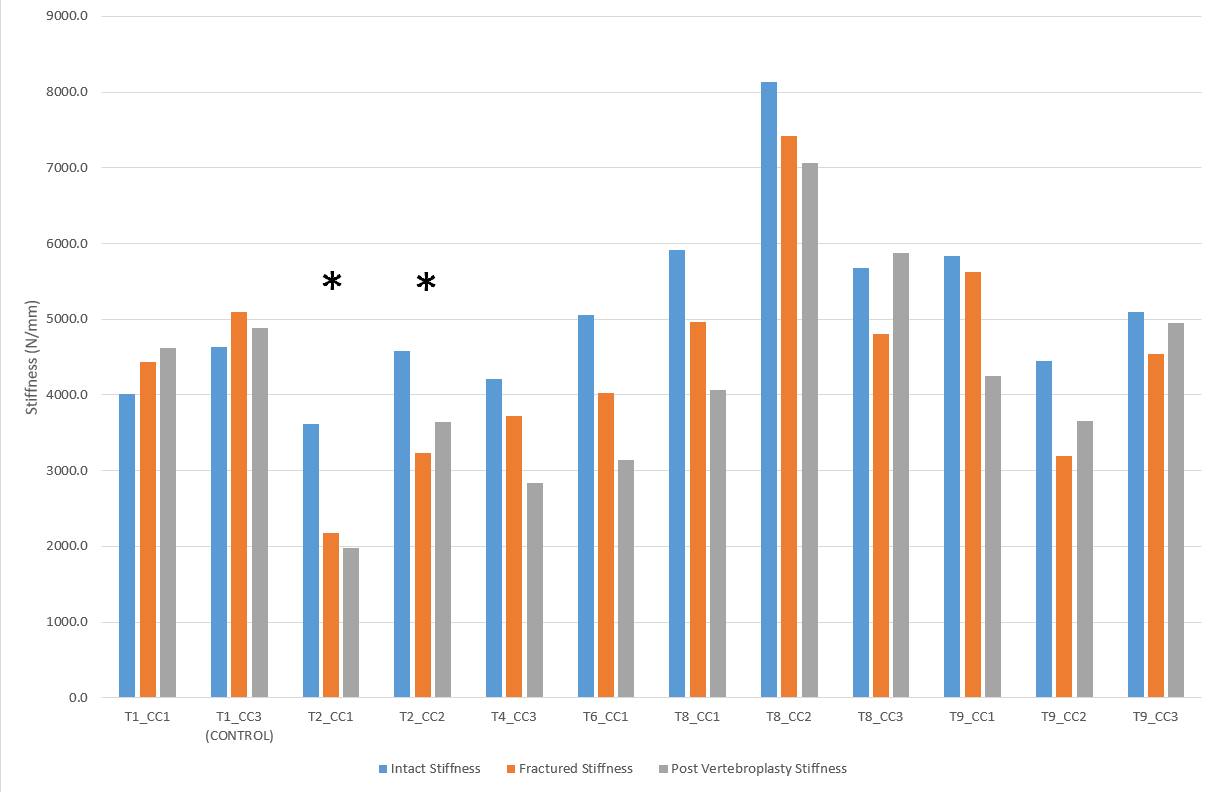
\includegraphics[width=\textwidth]{images/All_experimental_Data.png}
\caption{The maximum stiffness of 12 bovine tail vertebrae between 0 and 5000 N taken from load - displacement data. Showing the stiffness of the intact vertebrae, a post - fracture stiffness and a post - vertebroplasty stiffness for each. * Indicates those specimens that achieved a clear failure below 9500 N.}
\label{fig:allexpData}
\end{figure}

The results for the fill volume of cement in the augmented specimens is presented in \cref{tab:cementVol} and was acquired from the down-sampled, segmented models generated from $\mu$CT scans. It shows that fill volume varies between 3\% and 17\% fill and in addition shows a lack of a correlation between fill volume and increase in augmented specimen stiffness over fractured stiffness. \cref{fig:t2CC2vsT8CC2} shows the extent of the cement fill for the two vertebrae with the largest fill volume.

\begin{table}[ht]
\centering
\caption{The volume of cement and the vertebra volume for the 12 specimens used, along with the percentage cement fill and an indication as to whether the stiffnesses of the augmented vertebrae were greater than the fractured stiffness. This information was measured from the down-sampled models generated from $\mu$CT scans of the vertebrae.}
\label{tab:cementVol}

\begin{tabular}{l|>{\centering\arraybackslash}p{\dimexpr.16\textwidth}>{\centering\arraybackslash}p{\dimexpr.16\textwidth}>{\centering\arraybackslash}p{\dimexpr.16\textwidth}>{\centering\arraybackslash}p{\dimexpr.24\textwidth}}
Vertebrae & Cement Volume (mm$^3$) & Vertebra Volume (mm$^3$) & Cement Percentage of Vertebra Volume (\%) & Increase in Augmented Stiffness over Fractured Stiffness \\
& & & & \\ \hline \hline
T1 CC1 & 2260 & 32440 & 6.97 & * \\
T1 CC3 & 465 & 27039 & 1.72 &  \\
T2 CC1 & 663 & 23285 & 2.85 &  \\
T2 CC2 & 3405 & 20373 & 16.71 & * \\
T4 CC3 & 1363 & 25446 & 5.36 &  \\
T6 CC1 & 830 & 29332 & 2.83 &  \\
T8 CC1 & 1257 & 37357 & 3.36 &  \\
T8 CC2 & 4489 & 29248 & 15.35 &  \\
T8 CC3 & 1041 & 28403 & 3.67 & * \\
T9 CC1 & 2922 & 45681 & 6.40 &  \\
T9 CC2 & 2210 & 38894 & 5.68 & * \\
T9 CC3 & 2437 & 35840 & 6.80 & * \\ \hline
\end{tabular}%
\end{table}

\begin{figure}[ht]
\centering
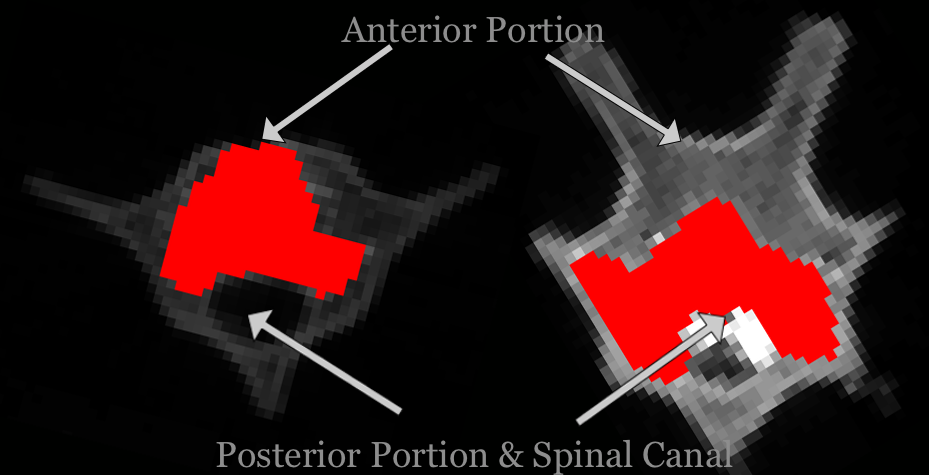
\includegraphics[width=4in]{images/t2CC2vsT8CC2.png}
\caption{$\mu$CT scans of T2-CC2 (left) and T8-CC2 (right), with cement masked in red, showing the extend of cement fill at the point where the cement was most anterior. }
\label{fig:t2CC2vsT8CC2}
\end{figure}

The attempt to reduce cement leaking through vasculature during the vertebroplasty procedure can be seen in \cref{fig:4vert_withBlutac}. The methods employed greatly reduced the the quantity of cement observed in both the spinal canal and around vascular channels at the vertebral body surface when compared to scans in \cref{fig:2vertWithoutBluTac}.

\begin{figure}[ht!]
\centering
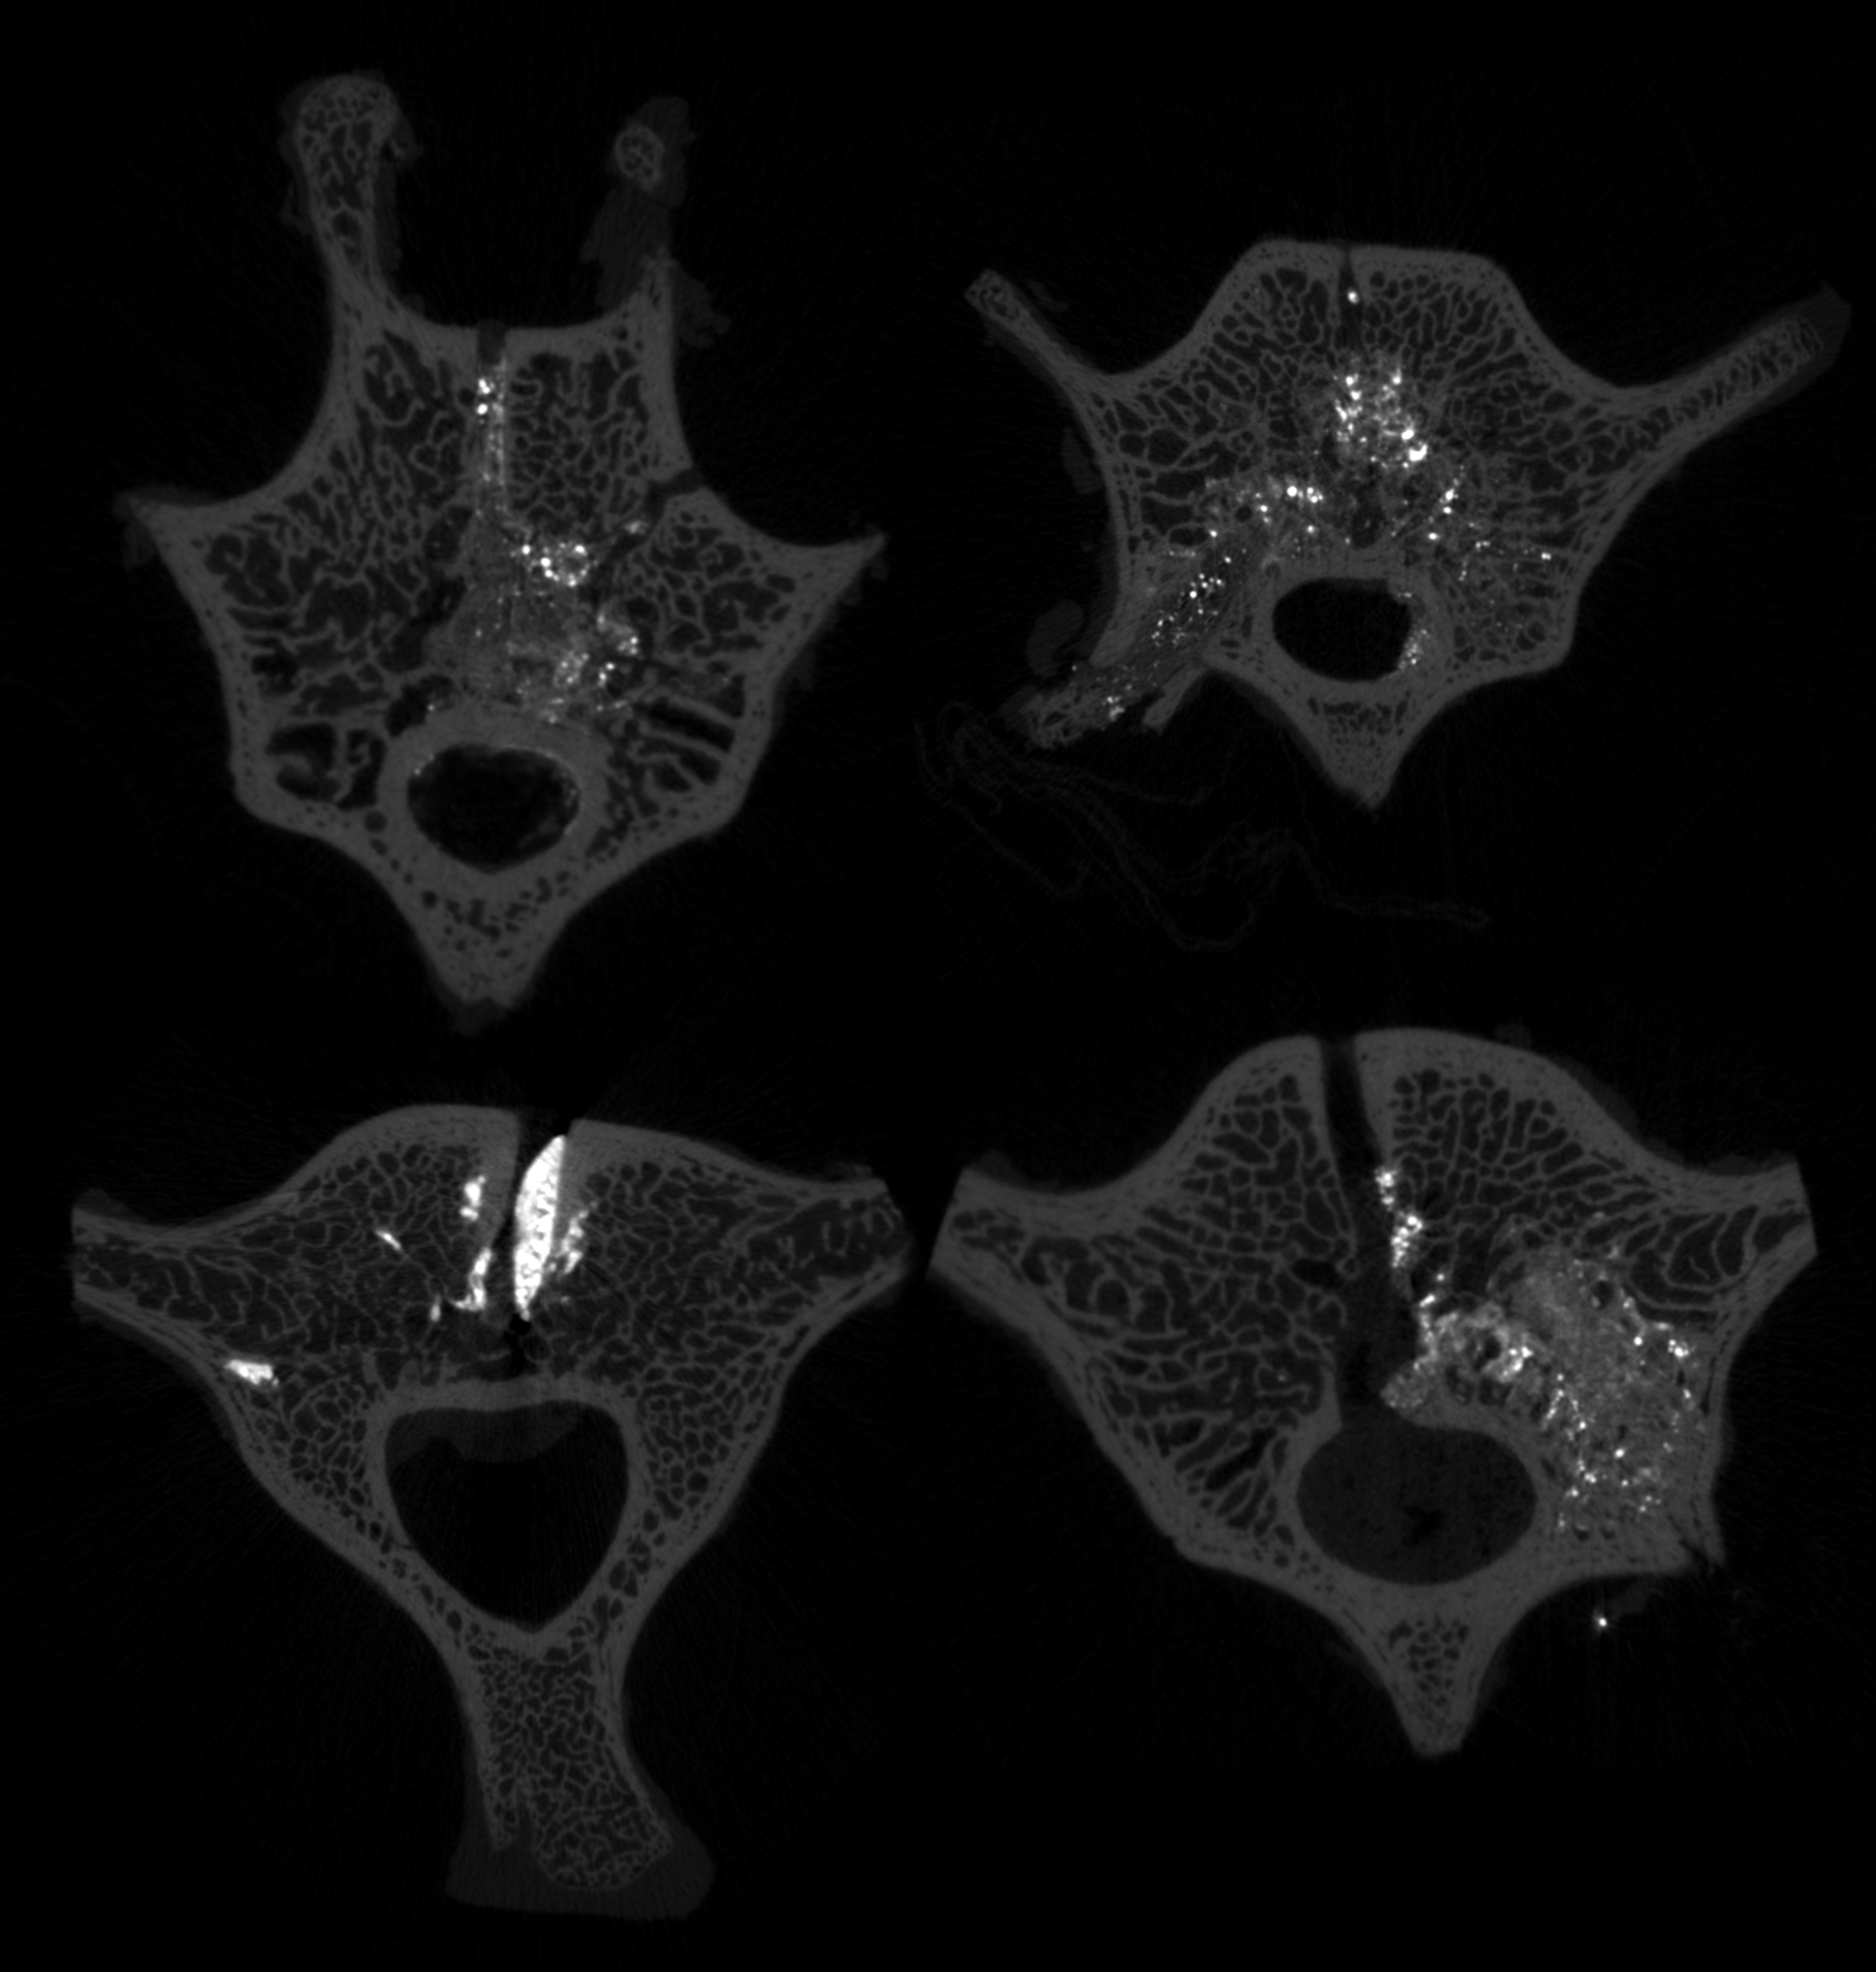
\includegraphics[width=3.8in]{images/4vertPostBluTac.png}
\caption{$\mu$CT scans of four augmented vertebra using a steel rod to fill the spinal canal and blu-tac to cover the external vascular channels. Shows greatly reduced cement content within the spinal canal with less cement at the surface of vascular channels.}
\label{fig:4vert_withBlutac}
\end{figure}


The two plots in \cref{fig:deltaStiffness_Vs_intact} show a lack of correlation between the difference in stiffness after augmentation when compared to both the fractured and intact specimen stiffness and the intact stiffness. Showing that magnitude of any increase or decrease in the vertebral stiffness following augmentation is not caused, or a feature of the initial, intact vertebral stiffness.

\begin{figure}[ht!]
\centering
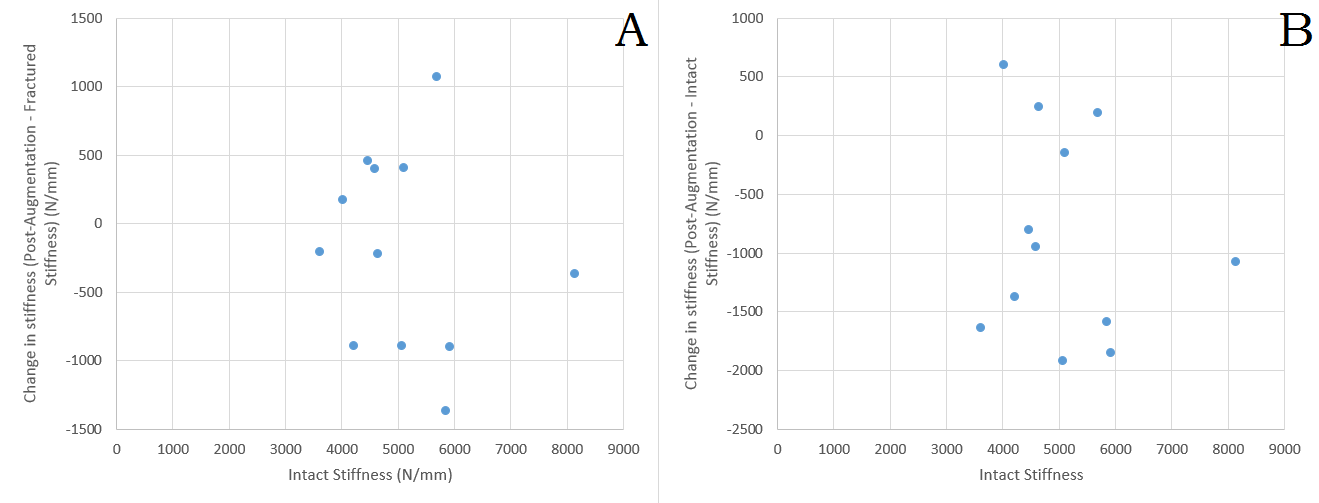
\includegraphics[width=\textwidth]{images/deltaStiffnessVsIntact.png}
\caption{A: The difference between the post augmentation and fractured stiffness against the intact stiffness. B: The difference between the post augmentation and intact stiffness against the intact stiffness.}
\label{fig:deltaStiffness_Vs_intact}
\end{figure}

\subsection{Discussion}\label{discussion-bov}

The experimental work carried out so far provides a good basis for both the continued modelling of vertebroplasty (especially modelling the cement - trabecular interface which is discussed in later sections) and to continue the experimental work using human tissue. Understanding the challenges of vertebroplasty (those discussed above), will be invaluable when transitioning onto the much more limited sou nrce of human vertebrae.

%^ reiterate aims of exp work

Regarding the results of stiffness at the intact, fractured and augmented stages, the expected trends were not always clear. Most commonly the intact vertebrae have the greatest stiffness with the fractured stiffness showing a reduced value following the damage created with the initial load to failure. The variation of the decrease (and increase) in stiffness for the fractured vertebrae may have a variety of reasons, although the most likely cause is level of damage caused in the initial ``load
to failure''. These tests varied between the typical load displacement that includes a failure (\cref{fig:failure_non_failure}:A) and those that show no sign of failure up to the limit of the load cell (\cref{fig:failure_non_failure}:B). It is difficult to observe any correlation between these vertebra that showed clear failure (T2-CC1 and T2-CC2), those that reached 9500 N and a reduction in the fractured stiffness. It is not to say that the vertebra that reached 9500 N experienced no damage, with the gradient of the load displacement curve often reducing and plateauing as the 9500 N limit approached. The interesting increase in the fractured stiffness for T1-CC1 compared to the intact stiffness may be explained if it is assumed that the compacted trabeculae following the first load to 9500 N result in a stiffer material for the following tests.

The cement fill volume information shows that a small percentage of cement is injected into the vertebrae on average, with only two vertebrae approaching the clinically relevant 20\% fill. Unexpectedly, only one of these two vertebrae showed an increase in augmented stiffness over the fractured stiffness. A possible explanation is that it is not only the fill volume that is important in restoring the vertebral stiffness but the placement too. This is shown when comparing the segmented scans of the the two vertebrae with the greatest fill volume with the T2-CC2 specimen showing cement extending to the anterior wall of the vertebral body, while the cement is limited to the posterior and centre of the vertebral body for T8-CC2. This may help to explain why the stiffness of T8-CC2 did not increase following augmentation. The reduction in stiffness following augmentation for seven of the twelve vertebrae may be due to damage caused by the insertion of vertebroplasty needles. Clinically this damage left behind from the needle channels would heal, most likely restoring the stiffness of the vertebrae back to its intact properties.

Another possible area of inconsistency is the temperature at which the vertebra were mechanically tested, while it is ensured that the specimens were fully defrosted they were tested at both fridge temperature (4$^\circ$C) and room temperature (20$^\circ$C). The effect of this variation in temperature needs to be identified and depending on the results more closely monitored.

Despite encouraging results regarding the vertebroplasty methodologies it was difficult to achieve the desired quantity of the cement in the vertebral body. This was mainly due to the difficulty injecting the cement in a smooth manner, which may have been caused by either the tip of the needle becoming blocked following its reinsertion into the needle track, more viscous marrow stopping the displacement of less viscous marrow by the cement or compacted trabeculae around the needle channel that limit the flow of cement past them. One option to test in future work would be side opening needles, which would help guide the cement more accurately to the regions required while circumventing issue with the needle becoming blocked.

The experimental methods currently developed will be of great value when starting experimental work using human tissue albeit many will require adaption due to the differences between the tissue types. These include the density of the bone and methods of inserting the needles, where with the available human tissue being from the elderly, the bones will be most likely be osteoporotic. These bones will require more care to reach the correct region of the vertebral body with the needle and to ensure a clinically relevant volume of cement is used.


%Talk about extra plots in results - deltaStiffness and cement fill.

\pagebreak

\section{Finite Element Modelling
Methods}\label{finite-element-modelling-methods}

The aims of the finite element section of work were to develop methods that enable the creation of specimen specific models of vertebrae (both bovine tail and human). Initially the focus was on the generation of models that accurately describe the mechanical behaviour of intact bovine specimens, once this was achieved an attempt to model augmented specimens was made. In addition to these larger goals, certain sensitivity tests were carried out, including those to understand the effects that additional meshes have on model stiffness.

%^ introduction paragraph

\subsection{Model Creation}\label{model-creation}

The computational analyses of linear-elastic finite element models is
carried out using a combination the segmentation and meshing software, ScanIP (Simpleware, Exeter, UK) and the simulation software, Abaqus (Dassault Systemes, France). The $\mu$CT scans were converted into a
finite element mesh using the former software package, this was then
imported into the second piece of software to be configured and solved.

The scans acquired from the \(\mu\)CT scanner were converted from the ISQ
file format, generated by the scanner software, into the more portable TIFF image format files using an existing in-house  matlab script that
additionally converts the greyscale of the scan into 256 bins. This conversion from 16 bit TIFF files with 65,536 bins to 8 bit TIFF files was required due to the limitation to 255 material properties within Abaqus, this allows one greyscale value per material property (assuming all 255 greyscale values are represented in the scan). Once the
scan has been pre-processed it was imported into ScanIP ensuring
that the spacing of voxels was correctly set - in this case 82 \(\mu\)m.
Once imported, the location of the loading point was identified to
simulate the correct experimental load within ABAQUS; the marker (see \cref{fig:expsetup})
appears bright on the scan and its centre was taken as the load point,
calculated by converting the position into mm. This was achieved by
multiplying by the native resolution of 82 \(\mu\)m.

The following parts of model creation were carried out using a Python script from within the ScanIP software. The script carries out the process described below and was generated by the author by carrying out the process manually and in order to understand the steps required and then writing a script to perform those actions. The development of the script removed much of the user variation in the segmentation of each vertebral model.

\begin{figure}[ht!]
\centering
  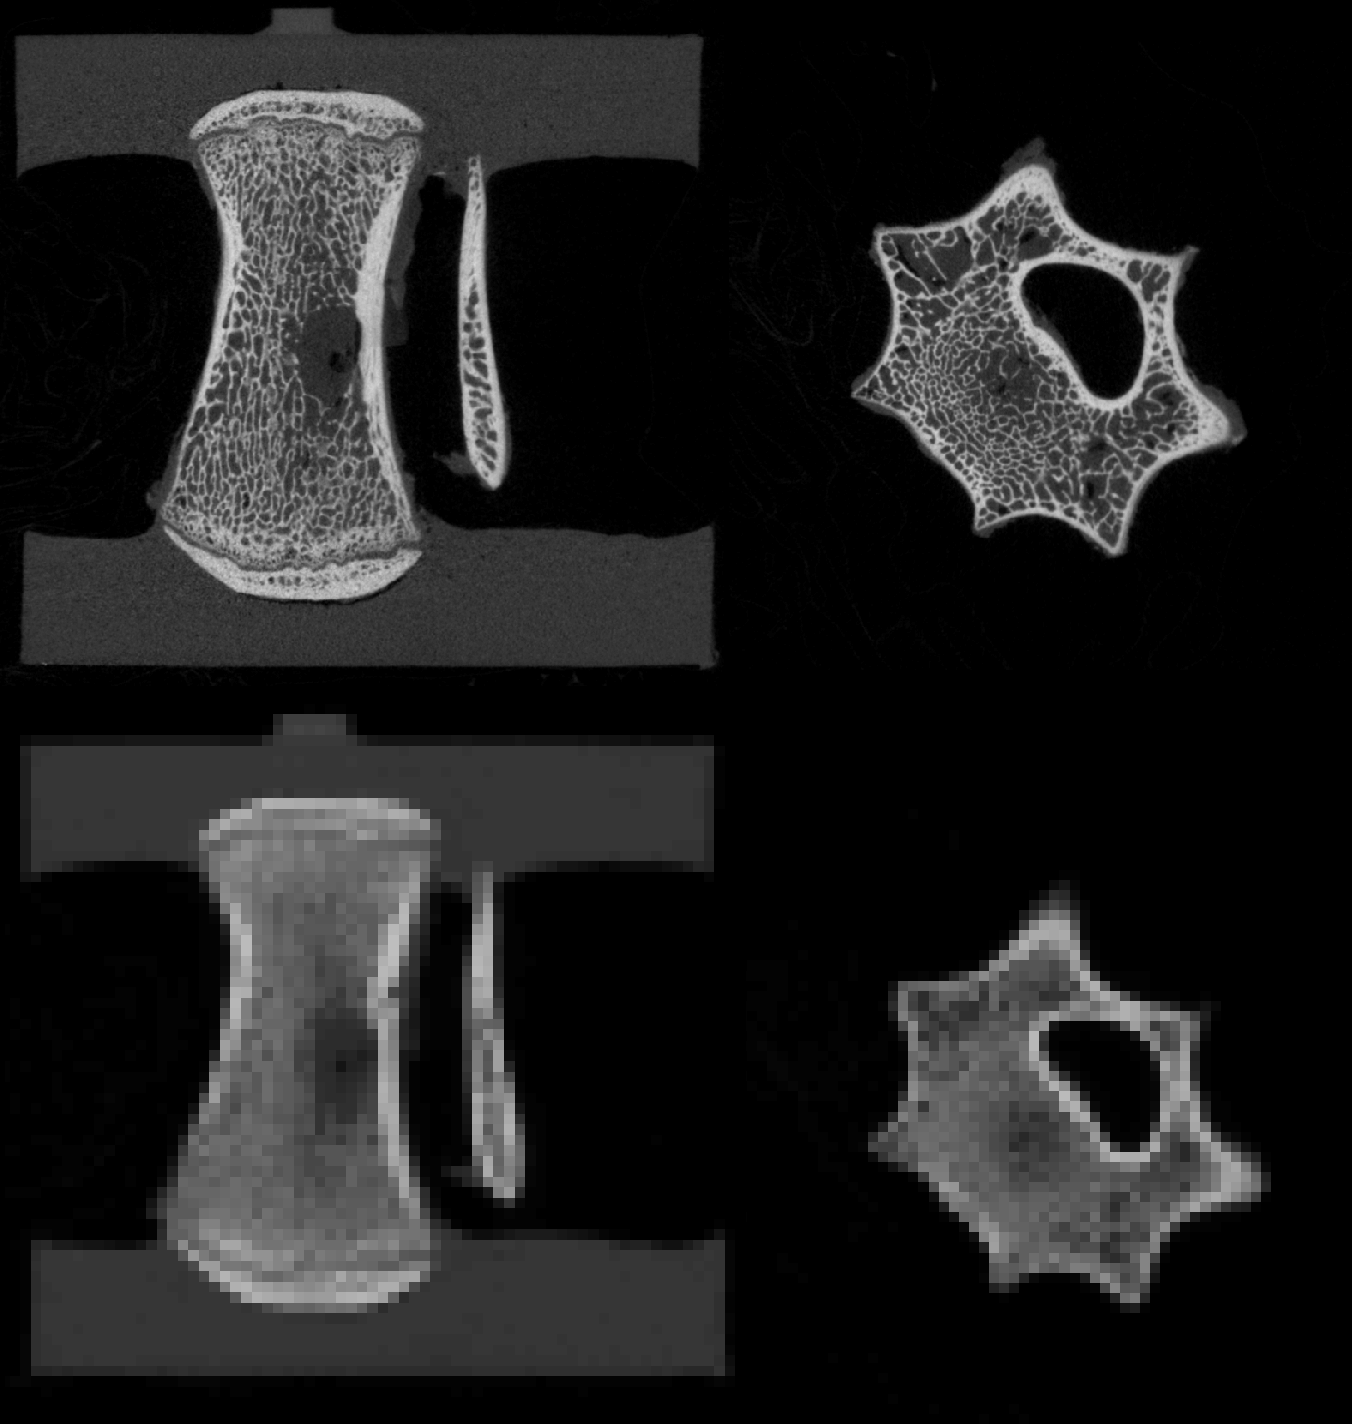
\includegraphics[width=4in]{images/compofDownsample.png}
  \caption{Side and top view of a vertebral $\mu$CT scan showing the effect of the downsample from 82 $\mu$m to 1mm cubed.}
\label{fig:compofDownsample}
\end{figure}




It was easier to down-sample the image stack prior to
segmentation, due to the time required for the software to generate
high resolution masks and increased memory usage at higher resolution. The effect of down-sampling can be seen in \cref{fig:compofDownsample}. However, in certain cases, for example when
modelling vertebral augmentation, in order to attempt to capture the
intricacies of the structure and the boundaries between cement and
trabecular bone it was favourable to generate the mask prior to down
sampling, \cref{fig:fullressVPseg}. The image stack was down-sampled to voxels 1 mm cubed, due to
previous studies producing sensitivity to mesh size results that showed
a good trade off between computational cost and model accuracy \cite{Jones2007}.



\begin{figure}[ht!]
\centering
  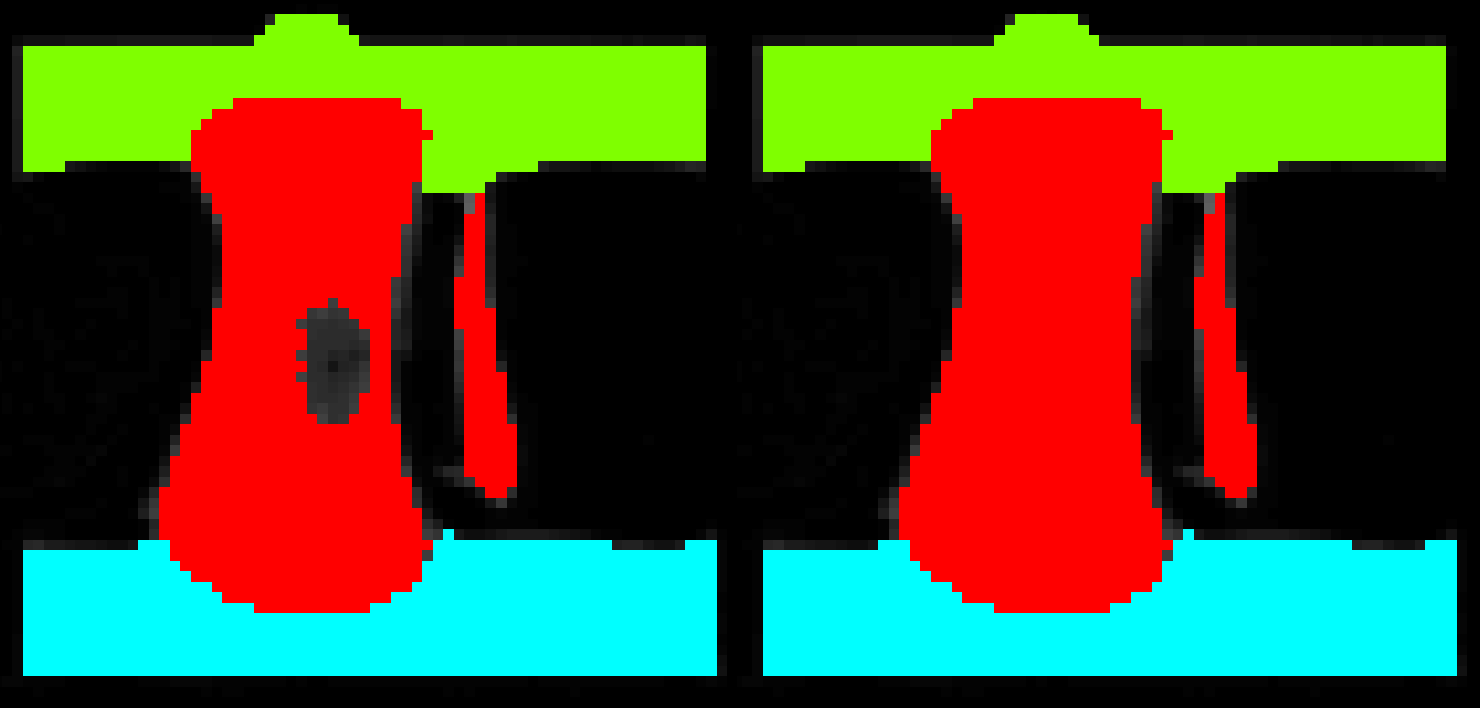
\includegraphics[width=4in]{images/fillTheVoid.png}
  \caption{Side view of a vertebral model showing segemented vertebra, including the internal void that is filled.}
\label{fig:fillTheVoid}
\end{figure}


Once down-sampled the image stack was segmented into the constituent
parts - the vertebrae and cement end-caps. The different regions that
were required to be segmented have different greyscale values, hence the
general shape of the masks was created through a thresholding tool that
selected volumes of the image stack between two bounds. For the end-caps
these bounds were usually between greyscale values of 12-22 and, if the
specimen was not augmented, the vertebrae between 23-255. For augmented
specimens these limits change to 23-65 for the vertebrae and 66-255 for
internal cement containing barium sulphate. These values were selected by visually limiting the amount of unwanted material selected within the threshold and maximising the wanted material, for example - selecting as much of the end-caps as possible while limiting the selected background and vertebral material to a minimum. This thresholding can be seen in \cref{fig:fillTheVoid}.
 It was preferable to avoid
internal voids within each mask, due to the potential for errors that
can be thrown once the model is imported into ABAQUS, these were
removed with the use of the morphological close and cavity fill tools within ScanIP (\cref{fig:fillTheVoid}).





The following parts of the method were carried out manually, following the completion of the automatic segmentation python script. The two end-caps were separated into two
separate masks by first duplicating the mask and then flood filling each end-cap to form separate masks.

An FE model was created using the previously generated masks and properties for the volume meshing, materials and contacts were set. The grid size for the model was set to 1 $\times$ 1 $\times$ 1 using the FE grid algorithm which uses a mix of tetrahedral and hexahedral elements. Material properties were set to homogenous with a density = 1, Young's modulus = 2.45 (GPa) and Poisson's ratio = 0.3 for the end-caps and when appropriate, were set to the internal cement volume. The material
properties for the vertebral volume were set to a greyscale based material type using the greyscale background information. The coefficients were set so that both the density and Young's modulus were equal to the greyscale value for that element, allowing the Young's modulus to be set correctly in following steps and as described in Section \ref{material-properties-bov}.

Contacts were set as placeholders to be edited in Abaqus in the steps following. These were contact pairs between each component and another between the superior end-cap and the upper boundary on the Z-axis. The second contact type was a node set between the inferior end-cap and the lower boundary on the Z-axis.

\begin{figure}[ht!]
\centering

  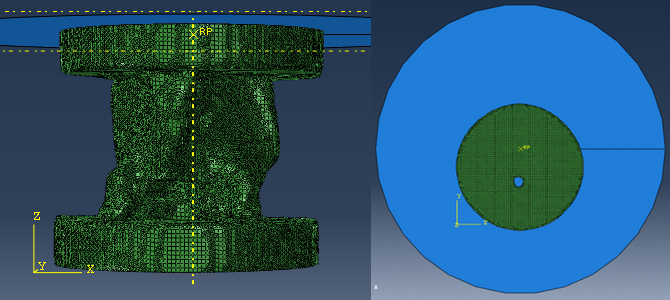
\includegraphics[width=4in]{images/abaqus_side_view_Both.png}
  \caption{Side \& top down view of a vertebral model showing the alignment of the analytical rigid plane.}
\label{fig:abaqus_top_view}
\end{figure}


Following this, the FE model was meshed, then exported into an INP file format. The model was then imported into Abaqus where the following configuration was completed by a second python script. An analytical rigid plate was created to represent the upper loading platen of the materials testing machine and was centred at the loading point previously found from the marker, this can be seen in \cref{fig:abaqus_top_view}. Once aligned any previous placeholder interactions were removed and a tied interaction was created between the rigid plate and the superior end-cap, along with tied interactions between the vertebra and both end-caps and, if appropriate, to the internal cement volume. An encastre boundary condition was created at the bottom surface of the inferior end-cap removing all rotational and translational movement and therefore mimicking the experimental setup. A displacement boundary condition was applied to a reference node at the centre of the rigid plate and therefore loading position, the properties were set such that 1 mm of displacement occurs in the negative Z direction; lateral motion in the X and Y planes was restricted, while rotation about the loading point was allowed - again mimicking the experimental setup.

The python script was written to set the material properties of the greyscale dependant vertebral elements by setting the Young's modulus to the greyscale value multiplied by a conversion factor (which is discussed in section \ref{material-properties-bov}). The script allowed Abaqus to solve the models and outputs the stiffness for each model. This was calculated by the dividing the reaction force at the reference point by the displacement at 1 mm of displacement.

\subsubsection{Augmented Model Generation}

In order to attempt to capture the detail of interdigitation between the
vertebrae and the injected cement, the masking process was carried out prior to downsampling, seen in \cref{fig:fullressVPseg}. If masked post-down-sample it became difficult to define the cement boundaries and the masked volume was inaccurate when compared to the full resolution scan.


\begin{figure}[hbt]
\centering

  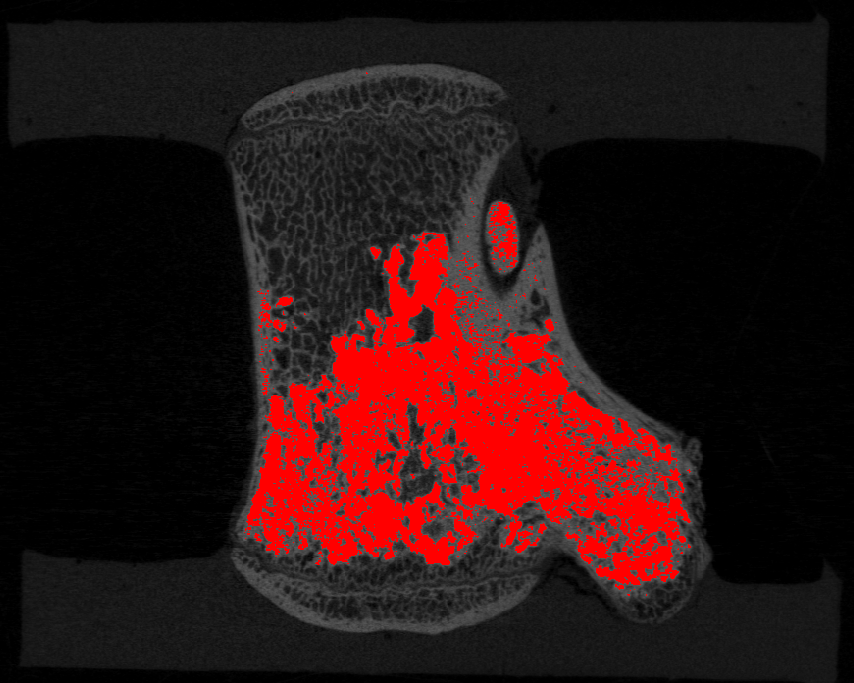
\includegraphics[width=10cm]{images/fullres_VP_segment.png}
  \caption{A lateral slice through an augmented bovine tail vertebra, showing
the cement mask in red.}
\label{fig:fullressVPseg}
\end{figure}


\subsection{Material Properties}\label{material-properties-bov}

Material properties for the bone tissue were modelled elastically using a
bone element-specific elastic modulus (\(E_{\text{ele}})\) that is
dependent on the average greyscale value for the element in question
(\(\text{GS}_{\text{ele}})\) with the conversion factor between the two being $\alpha$.

\[E_{\text{ele}} = \alpha\ \text{GS}_{\text{ele}} (GPa)\]

This was required due to each element containing differing quantities of bone and bone marrow due to the continuum level modelling carried out. Hence, a homogenous value for the trabecular bone would not have represented the varying average of material properties seen in each element. Therefore, the conversion factor, $\alpha$ was used to convert between the greyscale value for each element and the Young's modulus.

This work was carried out in parallel to that described in the experimental sections above, however the experimental and computational methods remained the same. Specimens were divided into two groups of twelve  and were used to determine a conversion factor between greyscale and elastic modulus. This additional set of 24 specimens (separate to
those used in the above experimental study) was worked on in collaboration with Dr Sebastien Sikora, Dr Fernando Zapata Cornelio \& Ruth Coe (Research Fellow, Research Fellow \& PhD student respectively).
The groups consisted of a calibration group (used to determine the value of $\alpha$) and a validation group. For the validation group material properties were assigned - multiplying the greyscale
for each element by \(\alpha\) prior to compressing the model by 1 mm in
Abaqus and was used to validate against the experimental values of stiffness.

The calibration for \(\alpha\), the conversion factor was carried out
using a golden section search scalar optimisation process. Specifically
using the Brent method within the opti4Abq toolbox (Marlene Mengoni, University of Leeds). The objective of this toolbox was to find the root mean
square normalised difference between the experimental specimen stiffness
and the finite element stiffness and iterate until the objective
function achieved a value of 10\textsuperscript{-3}.

\subsubsection{Augmented Specimen Material
Properties}\label{augmented-specimen-material-properties}


For convenience the values for the Young's modulus for the interior cement volume were initially set to that of the inferior and superior end-caps. However, due to the rule of mixtures and the results found in the literature \cite{Kinzl2012a,Race2007}, the effect of reducing the Young's modulus was investigated. This was carried out by reducing the Young's modulus in 10 percent increments from a value of 2.45 GPa to 1.225 GPa.


\subsection{Sensitivity Tests}\label{sensitivity-tests}

\subsubsection{Mesh Size Sensitivity}\label{mesh-size-sensitivity}

Element sizes of 1 x 1 x 1 mm were used throughout, following previous
convergence studies on porcine vertebrae \cite{Jones2007}. The
results of the convergence study on porcine vertebrae showed that reducing the element
size below 2 x 2 x 2 mm led to changes in the model that were smaller
than predicted errors originating from other factors, such as
experimental errors and the simplification of boundary conditions.
However, reducing the element size to 1 x 1 x 1 mm allows greater
resolution when modelling the intricacies of the cement mesh for
augmented specimens, the difference between the two resolutions can be
seen in \cref{fig:vertslice}.

\begin{figure}[ht!]

\centering
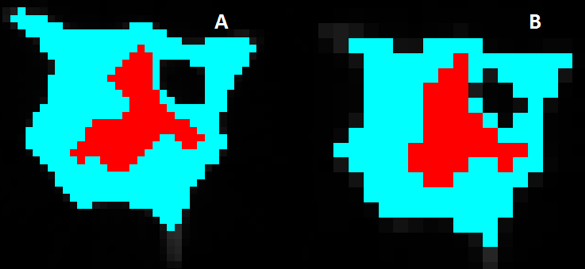
\includegraphics[width=3.90994in,height=1.80208in]{images/res_comp.png}
\caption{Mid-slice through an augmented vertebra, cyan: vertebral body, red:
cement. A, element size of 1 x 1 x 1 mm. B, element size of 2 x 2 x
2 mm.}
\label{fig:vertslice}
\end{figure}

\subsubsection{Addition of Cement}\label{addition-of-cement}

\paragraph{Sensitivity to an Additional
Mask}\label{sensitivity-to-an-additional-mask}

The addition of cement into the vertebral body created an extra mesh boundary
within the mesh containing the vertebral elements. In order to test what
effect this may have on the stiffness of models containing an extra
mesh boundary, an un-augmented specimen was tested with an extra mesh
representing the cement, but with the material properties of its
elements set based on their greyscale as with the other bone elements.
The mask was created by duplicating the vertebral mask and eroding it
until the volume was approximately 20 \% of its original volume. This
allowed testing to be carried out on the effect of the extra mesh alone,
while using an augmented specimen would allow a more accurate cement
shape, it would hinder setting material properties to that of the bone
greyscale and create an additional level of uncertainty. Mesh
interactions between the two meshes (internal vertebral surface and the
cement mask surface) were set using the contact pair interaction and
treated similarly to the interaction between the end-caps and the
vertebrae. Following model setup in ABAQUS as outlined in section \ref{model-creation} the model
was loaded in compression to 1 mm and its stiffness was recorded.

There was no difference between the two models, with and without the
internal cement mesh, meaning that any changes to the augmented model
stiffness was due to the material properties of the cement.

\paragraph{Mesh Interactions}\label{mesh-interactions}

The effect of mesh interaction between the vertebral body and the
internal cement mesh were tested by comparing a) tied interactions
between the two surfaces and b) removing any interaction and merely
changing the material properties of the internal cement region
(neglecting the contact pair steps described earlier). This was carried
out for four augmented specimens following the same setup within ABAQUS
as described earlier.

The results can be seen in \cref{tab:meshint}, showing a negligible
difference
between variations for the four vertebrae models. This difference falls
well below the difference between experimental and computation,
especially for the augmented specimens, hence the effect of this
interaction can be neglected from further test.

\begin{table}[ht!]

\caption{The difference between interaction properties, tied and not tied for
four augmented vertebrae specimens.}
\label{tab:meshint}
\centering
%\resizebox{\textwidth}{!}{
  \begin{tabular}{c|c|c|c}
Vertebrae (Tail Number,  & Tied Interaction  & No Tied Interaction  &
Difference \\
Vertebral Level) & (N/mm) & (N/mm) & (\%) \\
\hline
\hline

T2 CC1 &	 5496 &	 5496 &	 0\\
T2 CC2 &	 8086 &	 8086 &	 0.001\\
T6 CC1 &	 3686 &	 3686 &	 0.001\\
T4 CC3 &	 6059 &	 6059 &	 0.0005\\ \hline

\end{tabular}
%}
\end{table}



\subsubsection{Augmentation Volume \& Location Sensitivity}






\subsection{Results} \label{bov:results}

The optimisation process gave a value for the conversion factor of 0.012529, allowing conversion between greyscale values for elements and their elastic modulus. This value was used for the bone constituents of the intact and augmented vertebrae presented in \cref{fig:compvexpscatter}, which shows the agreement between the \textit{in vitro} and \textit{in silico} results for the specimen specific models. The agreement of intact vertebrae was considerably better, with a concordance
correlation coefficient (CCC) of 0.49 compared with 0.16 for the augmented vertebrae (\cref{tab:int}), with the value increasing to 0.60 if the uncharacteristically stiff T8-CC2 was removed.

\begin{figure}[ht]
\centering
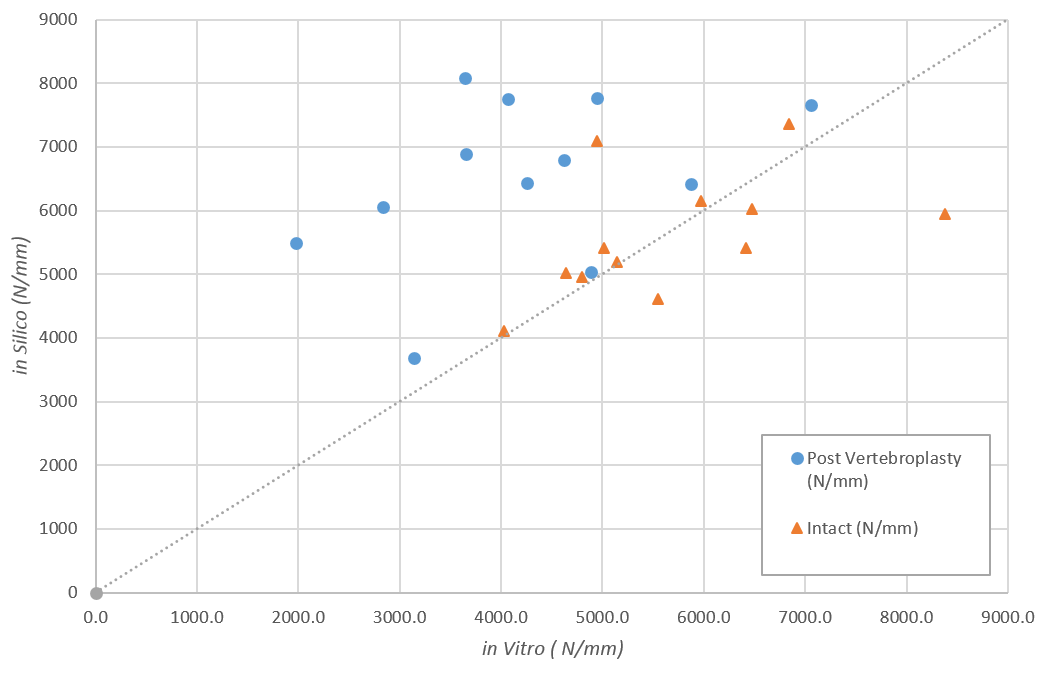
\includegraphics[width=\textwidth]{images/exp_vs_comp_both.png}
\caption{\textit{in silico} compared with \textit{in vitro} stiffness for intact specimens (triangles) and augmented specimens (circles). The dotted line shows a one-to-one correspondence.}
\label{fig:compvexpscatter}
\end{figure}

\begin{table}[ht]
\centering
\caption{The mean, standard deviation and concordance correlation coefficient (CCC) of the intact and augmented vertebrae for \textit{in vitro} and \textit{in silico results}.}
\label{tab:int}
\begin{tabular}{l|c|c|c}
     Intact Specimens     & Mean Stiffness & Standard Deviation & CCC                     \\ \hline \hline
\textit{in vitro}  & 5684 & 1196             & \multirow{2}{*}{0.4895} \\
\textit{in silico} & 5610 & 958               &                        \\
\hline
 Augmented Specimens
 \\ \hline \hline
\textit{in vitro}  & 4246 & 1371               & \multirow{2}{*}{0.1548} \\
\textit{in silico} & 6507 & 1298               &                      \\ \hline
\end{tabular}
\end{table}

The effect of changing the modulus of the cement volume in the augmented specimens is presented in \cref{fig:redEModBar}. There was a linear decreases in the stiffness of vertebrae with the reduction of he elastic modulus for the internal cement volume. The two vertebrae that show more prominent decreases in stiffness were those vertebrae that contained larger volumes of cement following their augmentation.

The effect that this has on the data with regard to the \textit{in vitro} stiffness results can be seen in \cref{fig:redEModscatter}, where the reduction in \textit{in silico} stiffness moves the data points closer to the $x = y$ line of perfect agreement between the experimental and computational results.


\begin{figure}[ht!]
\centering
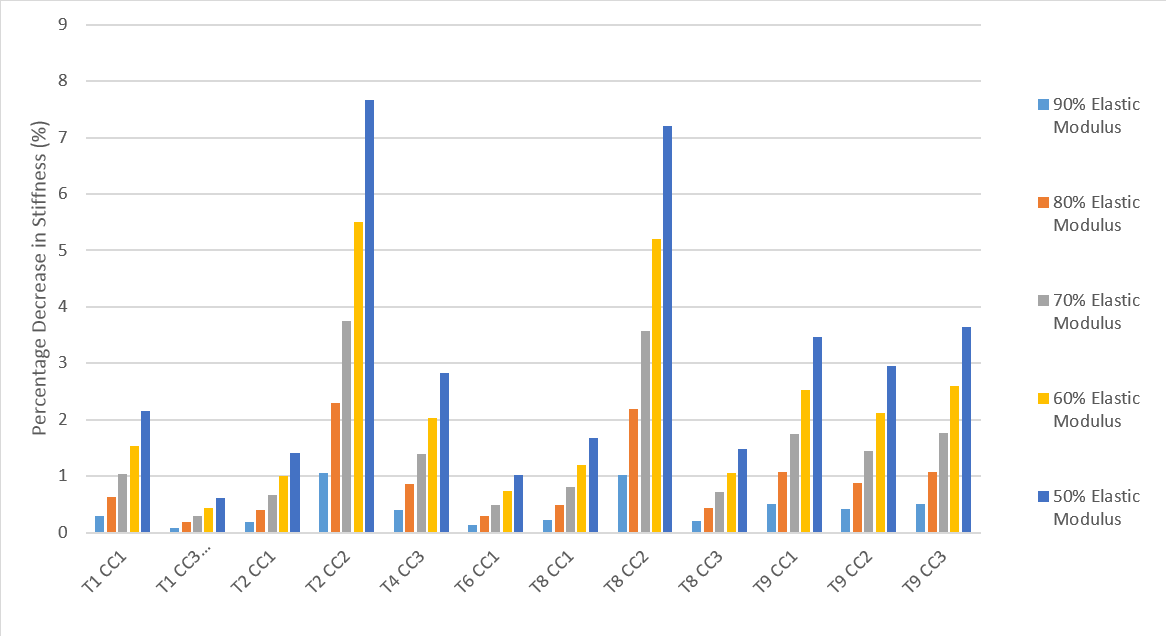
\includegraphics[width=\textwidth]{images/reductionOfEMod_Bar.png}
\caption{The percentage decrease in the vertebral stiffness after reducing the elastic modulus of the cement volume within 12 augmented vertebrae.}
\label{fig:redEModBar}
\end{figure}

\begin{figure}[ht!]
\centering
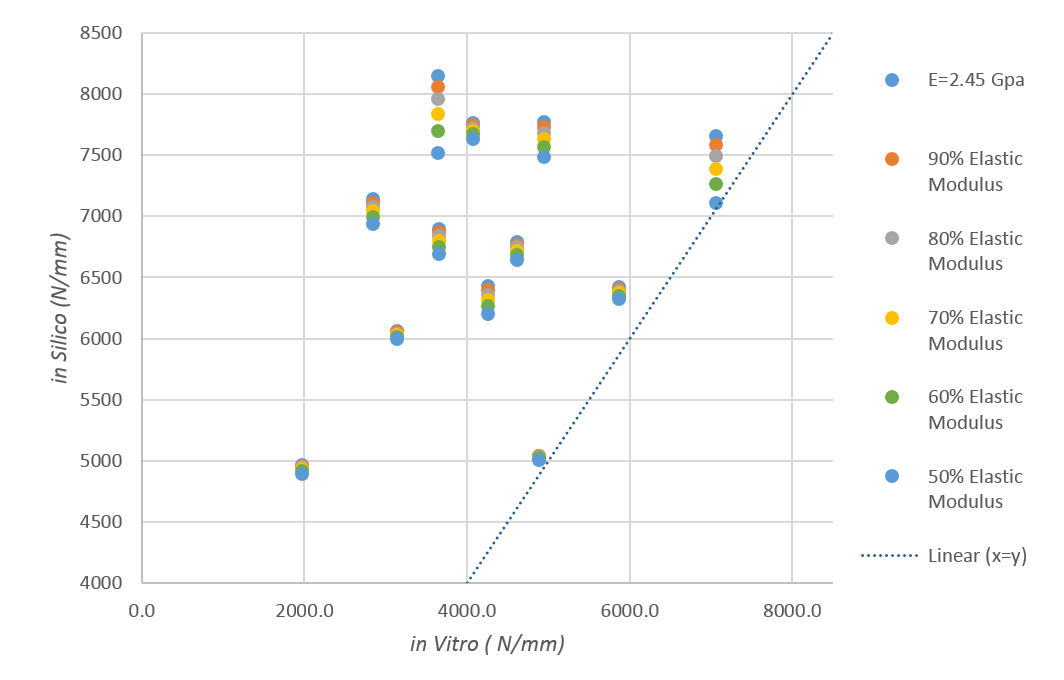
\includegraphics[width=5.3in]{images/reductionOfEMod_Scatter.png}
\caption{The effect of reducing the elastic modulus of the cement volume within 12 augmented vertebrae. Shows the in silico stiffness for the six elastic moduli tested against their in vitro stiffness. }
\label{fig:redEModscatter}
\end{figure}

\pagebreak

\subsection{Discussion}

The computational methods developed and results acquired, as with the experimental results, provide a good base for using human vertebrae and for the continued development of augmented vertebra modelling. The methods and automation of the creation of models both greatly reduce the time spent on model generation and reduce human error. This allows a relatively easy translation to human vertebrae, with only minor adjustments to the thresholds that define materials.

The current methods of masking and meshing the internal volumes of cement in the augmented models provides a good method of creating augmented models. The sensitivity tests carried out on the additional mask inside the vertebrae shows that any effects seen are due to the volume of cement and not a simulation problem. Similarly the inclusion of a tied interaction between the two meshes failed to affect the result, something especially useful when considering alternative mesh interaction to model the cement - trabeculae interaction.

The intact models agree well with experimental results, with very similar results for the mean and, excluding anomalous results, a good CCC value,  showing that the previously validated conversion factor works well with this set of data and that segmentation and model setup works correctly. The poor agreement with the augmented specimen models and their experimental counterparts was an expected result that agrees with similar studies in the literature - \cite{Wijayathunga2008}. In an attempt to
produce a better agreement, the elastic modulus of the cement volume was reduced in accordance with the experimental results of Race et al. \cite{Race2007} and similar methods employed by Wijayathunga et al. \cite{Wijayathunga2008}, where the reduction in modulus is expected due to the greater ratio of monomer to powder used, gaps between the bone and cement and pores within the cement. The reduction in stiffness forms a linear pattern as the elastic modulus is reduced, with those vertebrae that
show the greatest reduction being those containing the largest volume of cement. While these results do show a reduction in the stiffness, closer to that of the experimental values, it does not explain the disagreement fully. This suggests that a combination of improvements to the augmented models is required.

Future work will utilise the results acquired, especially those relating to the cement modulus and the cement - bone interactions, to understand how to model this interface more realistically and achieve good agreement between experimental and computation results of stiffness for augmented specimens.



\chapter{Human Tissue} \label{Chapter_HT}

\section{Introduction}

Previous studies and earlier chapters have used a range of vertebrae, including
bovine, ovine and porcine among others. While all of these vertebrae have
important uses for developing methodology and understanding certain
characteristics, none share the trabecular structure, thickness of cortical
shell, axial strength of stiffness. Hence, in order to understand the
mechanical effects of vertebroplasty, human tissue is required.

Here, 14 lumbar vertebrae from four cadaveric spines have been used, with the
details shown in \cref{tab:vertebrae}.

\begin{table}[ht!]
\centering
  \caption{Details of the lumbar sections used from four cadaveric spines.}
  \label{tab:vertebrae}
  \begin{tabular}{c|c|c|c}
    Spine Name & Vertebrae & Sex & Age \\ \hline \hline
    Spine 1& L1, L2, L3, L4, L5 & F & 90\\ \hline
    Spine 2& L1 & F & 94\\ \hline
    Spine 3& L1, L2, L3 & M & 86\\ \hline
    Spine 4& L1, L2, L3, L4, L5 & M & 83\\ \hline

  \end{tabular}

\end{table}


\section{Experimental Methods}

\subsection{Dissection \& Potting}

The geometry of human lumbar vertebrae varies considerably to that of the bovine
tail vertebrae from which this methodology is based. This is characterised by
much larger posterior elements with the facets extending much lower, below the
bottom of the vertebral body. Hence, to correctly pot the human vertebrae much
more cement must be used, especially for the posterior end-cap, in order to
cover the bottom of the vertebral body and the extending posterior elements.
This means that much more of the posterior elements are constrained, therefore
restricting the rotation of the vertebral body endplates under axial load. In
addition to this the larger posterior elements which are captured within the
PMMA end-caps will transmit load and take a greater share of the load when
compared to the bovine tail vertebrae. Given that vertebroplasty attempts to
restore the stiffness of the vertebral body and that there is no understanding
of specifically how the loads are shared between the vertebral body and
posterior element, this presents a problem.

A solution to this is to remove the posterior elements, following such methods
as \cite{Wijayathunga2008,RobsonBrown2014}, where only the vertebral body is
modelled. This allows the stiffness of the vertebral body alone to be captured
and modelled. The posterior elements were removed by cutting through the
pedicles at the narrowest part, limiting damage to the region.

To pot the specimens that now lack a spinal canal, a retort stand was used to
hold the vertebra, ensuring that both endplates were level on average. The
specimen was then lowered down into the potting container leaving 5 mm between
the bottom of the vertebra and the container. PMMA was poured into the container
until the entire of the endplate was touching cement, with the edges of the
vertebral body covered. Care needed to be taken to ensure all of the endplate
was in contact with cement, given the extent of osteophytes creating non-flat
surfaces in some of the more degenerated specimens. The other side of the
vertebra was potted in a similar manner, however, due to the constraints of the
potting container a measured quantity of cement was poured prior to lowering the
vertebra into it. A spirit level ensured parallel end-caps.

\subsection{Loading}

Following previous studies \cite{Wijayathunga2008}, the vertebrae were loaded
with an initial maximum load of 800 N for similarly osteoporotic vertebrae.
However, after loading two of the initial set of vertebrae the stiffness
continued to increase up to maximum 800 N. Following loads up to 2000 N showed
that the stiffness reached a maximum between 1300 and 2000 N, with three of the
initial four specimens showing some degree of failure in the final 400 N of
loading.

\subsubsection{Maximum Stiffness Measurement}

The maximum stiffness of the vertebra was found in the same fashion as with the
bovine tail vertebrae - measuring the stiffness of segments at increments over
the length of the curve. Given that damage, especially for the intact specimens,
needs to be avoided the maximum loads used are on the conservative side. This
can mean that the maximum stiffness is potentially at the end of the data set or
that the stiffness is still increasing at the load cut off. The solution to the
latter would require a prediction of the yield point prior to experimental
loading (discussed in Section~\ref{predYield}), while the former could
potentially be solved by using smaller segment sizes when measuring the
stiffness from load - displacement results.

To allow the effect of segment size (the length of each section from which the
stiffness is found) and increment size (the size of each increment defining the
start point of each segment), the maximum stiffness finding Matlab code was
rewritten in Python. This function could then be iterated over, reporting the
maximum stiffness when using an increment size of between 1 and 100 data points
(the distance between two data points corresponds to 0.0017 mm). Changing the
increment size becomes a verification of the results using an increment size of
1 data point, given that the only negative of using the smallest possible
increment size is computational cost, which is negligible here.

\begin{figure}[ht!]
  \centering
  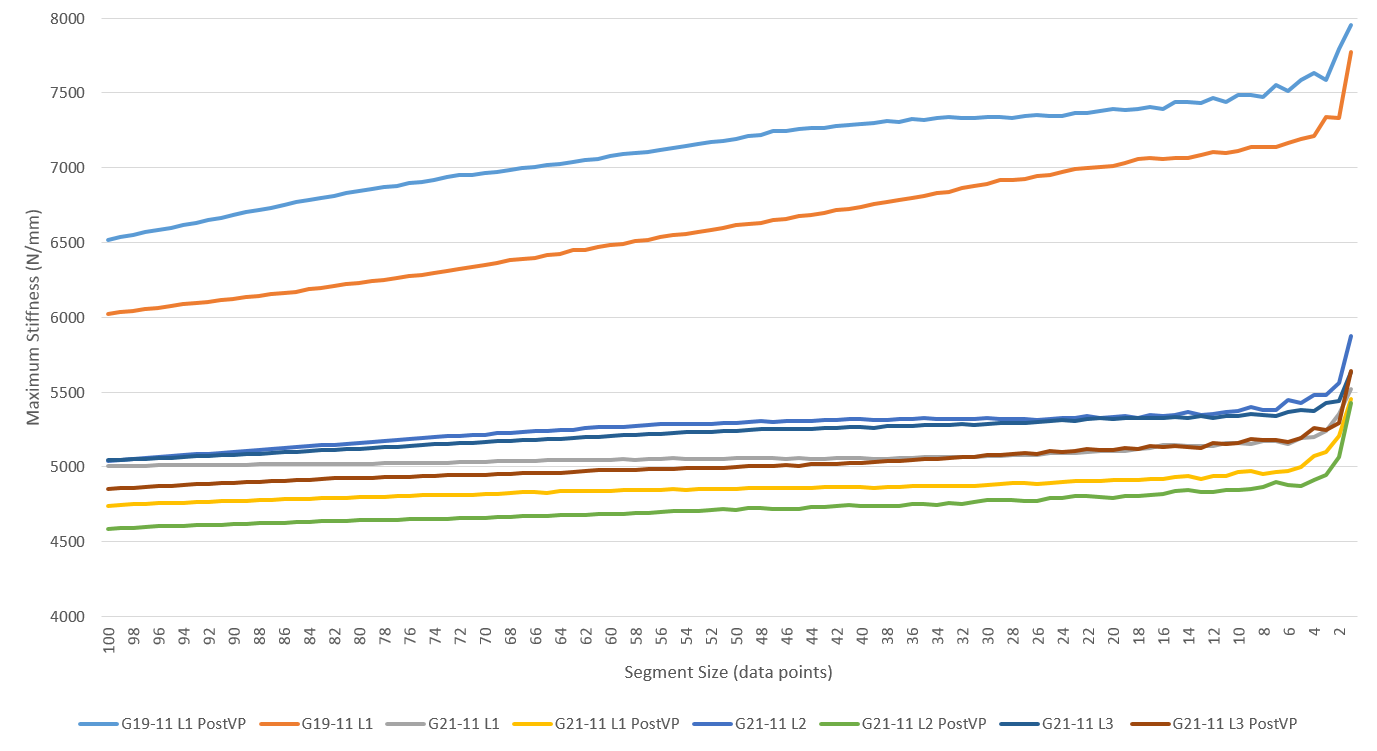
\includegraphics[width=6in]{Chapters/Chapter_HT_images/findStiffness_1incr.png}
  \caption{The effect of reducing the segment size on the maximum stiffness
    reported from four human vertebrae loaded to 2000 N pre and post
    augmentation. Using an increment size of 1 data point (0.0017 mm) and
    segment sizes of 100 to 1 data point (0.17 mm to 0.0017 mm).}
  \label{fig:findStiffness_1incr}
\end{figure}

\begin{figure}[ht!]
  \centering
  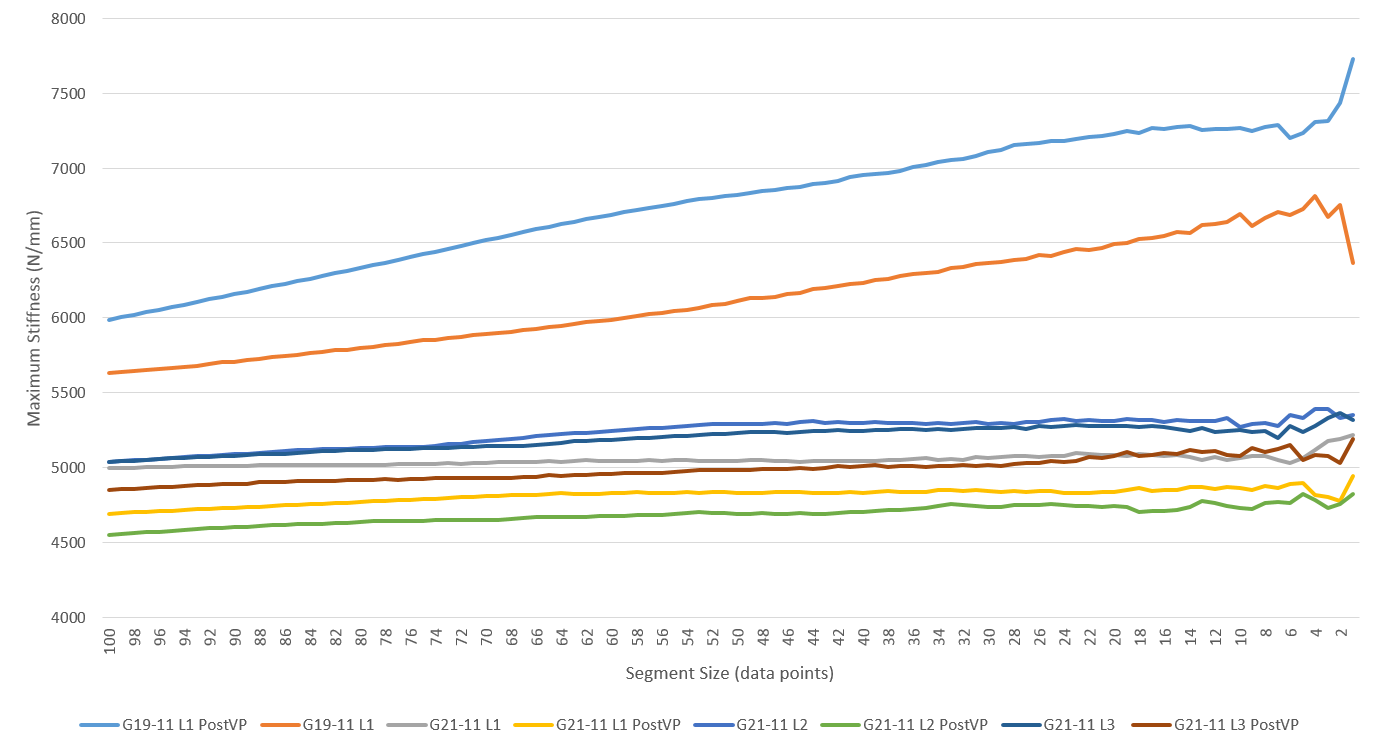
\includegraphics[width=6in]{Chapters/Chapter_HT_images/findStiffness_20incr.png}
  \caption{The effect of reducing the segment size on the maximum stiffness
    reported from four human vertebrae loaded to 2000 N pre and post
    augmentation. Using an increment size of 20 data points (0.0037 mm) and
    segment sizes of 100 to 1 data point (0.17 mm to 0.0017 mm).}
  \label{fig:findStiffness_20incr}
\end{figure}

Using an increment size of 1 data points width, as shown in \cref{fig:findStiffness_1incr} shows a smaller variation across the range of
segment sizes compared to using 20 points in \cref{fig:findStiffness_20incr}. The effect of both segment size and increment
size is especially evident for the two Spine 2 L1 vertebrae both intact and post
augmentation where the stiffness continues to increase until the end of the test
at 2000 N. Meaning that there is a much smaller linear region for these two
specimens, hence requiring a smaller segment size to measure the largest
gradient.

Choosing values for the segment size to use moving forwards becomes difficult
given the large effect it can have on the measured maximum stiffness (a range of
over 1000 N/mm in the case the two Spine 2 L1 tests). The segment size needs to
be small enough to capture the maximum stiffness while avoiding the noise when
using a segment size below 18 data points. Hence, a value of 20 data points was
chosen, a value that avoids the noise while being on the plateau of the lines.


\subsubsection{Repeated Loading}

Given the nature of the test (attempting to limit damage to the vertebrae)
especially during their initial intact load, the ability to derive errors
becomes difficult especially from a single load. To attempt to understand this
error four vertebrae having undergone augmentation were tested three more times
in an iterative fashion, removing each from the load testing machine, testing
the next specimen in the set and repeating. Removing the vertebrae from their
steel housing (instead of three tests while seated in the steel housing) allowed
the error in loading position and setup to be tested along with repeated loading
of the vertebrae to be tested.

The results of repeated loading can be seen in \cref{fig:exp_repeats}. All
four specimens show a reduced stiffness for the repeated loads following the
initial load, for which there are a few possible reasons. One possibility for
the reduction in stiffness is that it is a consequence of the freeze thaw cycle
that occurred between these tests. The second possibility is that the vertebrae
were still partially frozen while the testing took place. Finally, it could be
due to damage being caused during the initial load to 2000 N, shown in \cref{fig:Spine2_L1,fig:Spine3_L3} it is possible to see slight failure
in the three Spine 3 vertebrae, although failure cannot be seen in the Spine 2 L1
vertebrae. The frozen bar in \cref{fig:exp_repeats} shows how the
stiffness increases when the vertebrae are completely frozen, potentially
helping to explain the drop in stiffness found in the repeats. Further tests
will be carried out with three more repeats following another freeze thaw cycle
to attempt to answer this.

The iterative reduction in stiffness for the Spine 3 L2 vertebrae can be
explained as damage being caused after each iteration. This can be seen in
\cref{fig:Spine3_L2}, with the three repeats each showing a yielding
before the 1600 N limit and a smaller maximum load and stiffness after each
repeat.

Figures~\ref{fig:Spine2_L1} through~\ref{fig:Spine3_L3} show the data for the
loading, from which the maximum stiffness values are found. This excludes the
initial cyclic loading, starts the loading at 50 N and displacement at 0 mm.

\begin{figure}[!h]
  \centering
  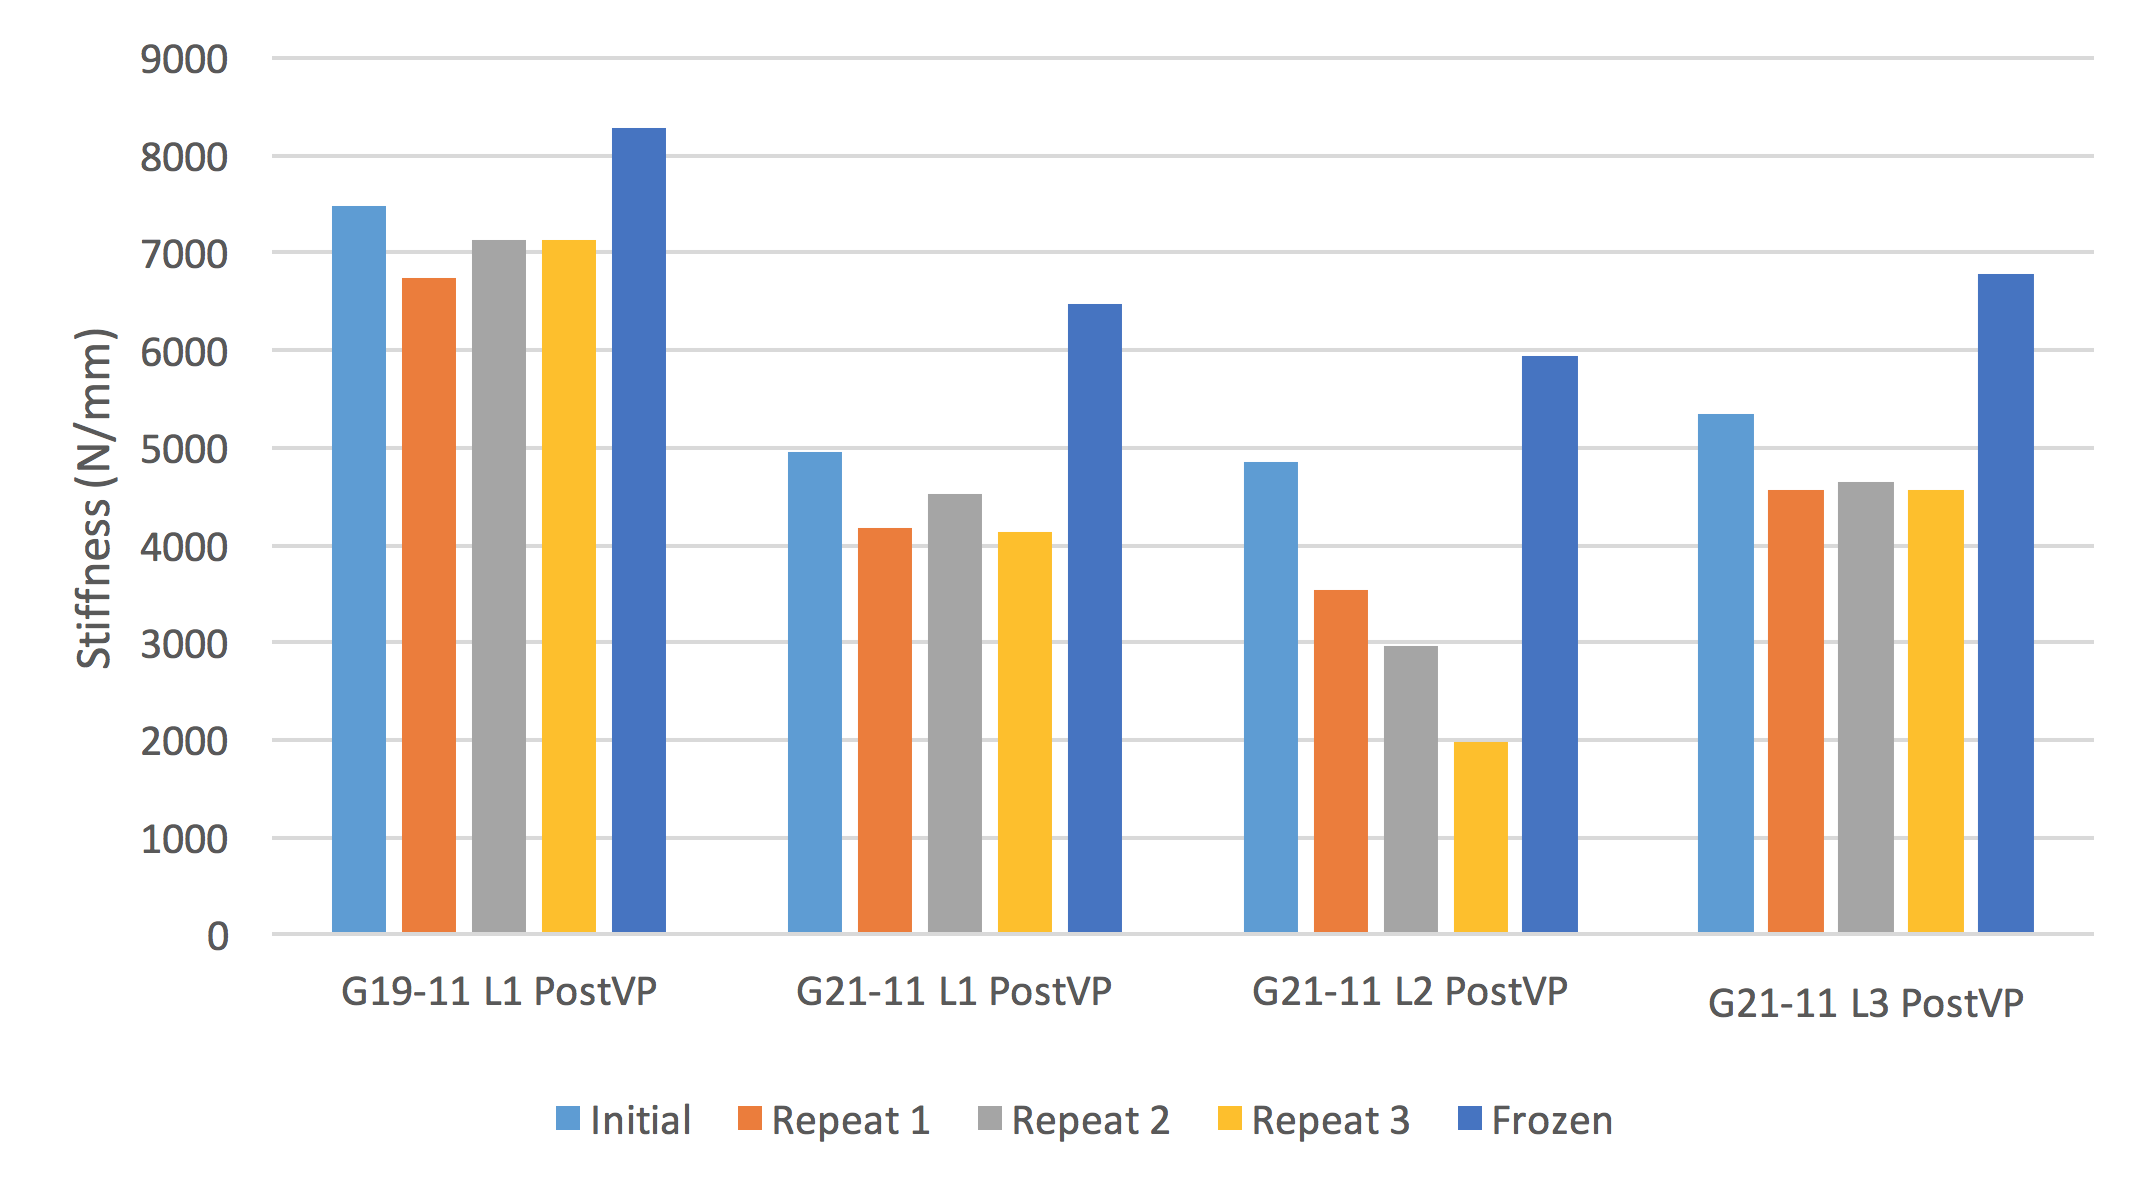
\includegraphics[width=6in]{Chapters/Chapter_HT_images/experimental_repeats.png}
  \caption{The stiffness of four augmented vertebral specimens over the course
    of an initial load, three repeated loads and a load while frozen. The intact
    specimen was loaded until 2000 N while the remaining four were loaded until
    1600 N.}
  \label{fig:exp_repeats}
\end{figure}


\begin{figure}[ht!]
  \centering
  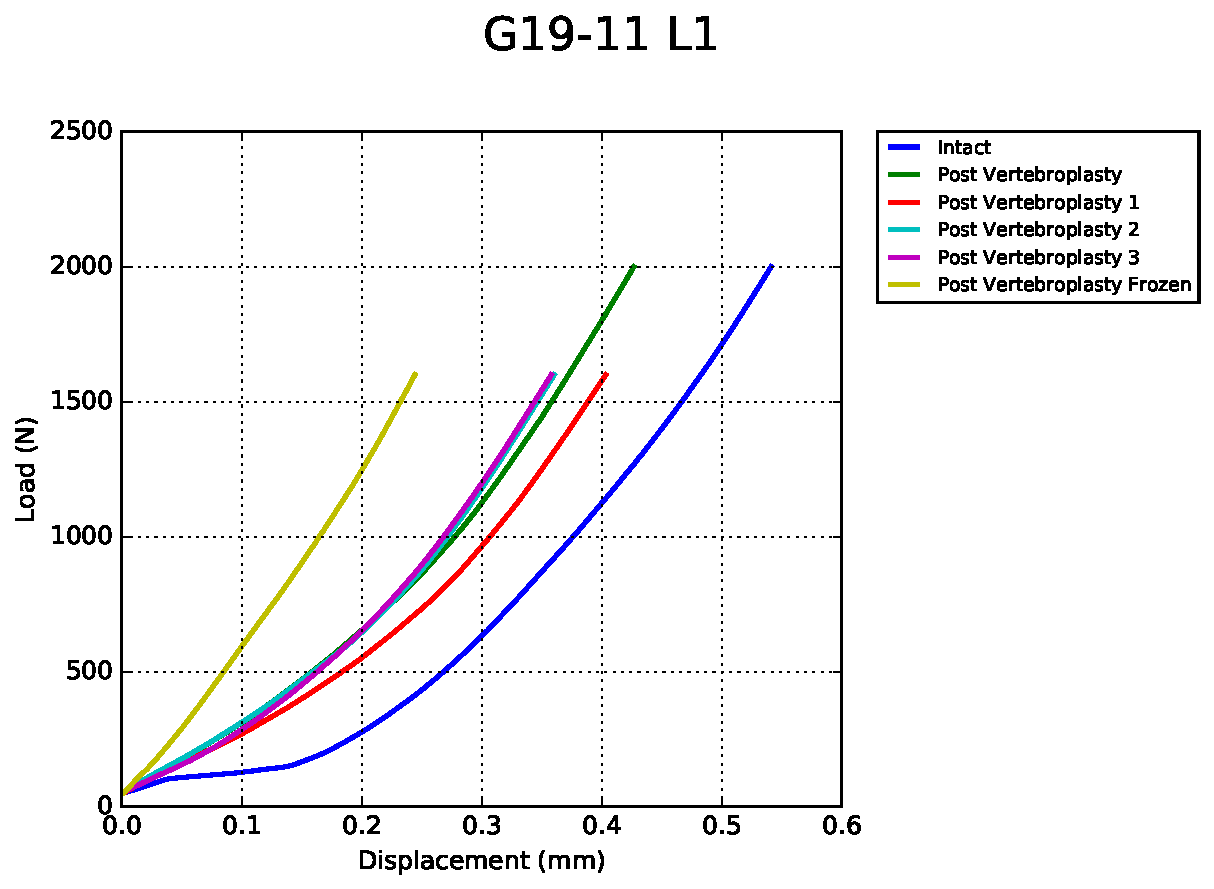
\includegraphics[width=4in]{Chapters/Chapter_HT_images/G19-11_L1.pdf}
  \caption{The load - displacement results for the Spine 2 L1 vertebra. Showing
    results of the intact load and post augmentation load up to 2000 N and the
    repeats and frozen load up to 1600 N.}
  \label{fig:Spine2_L1}
\end{figure}

\begin{figure}[ht!]
  \centering
  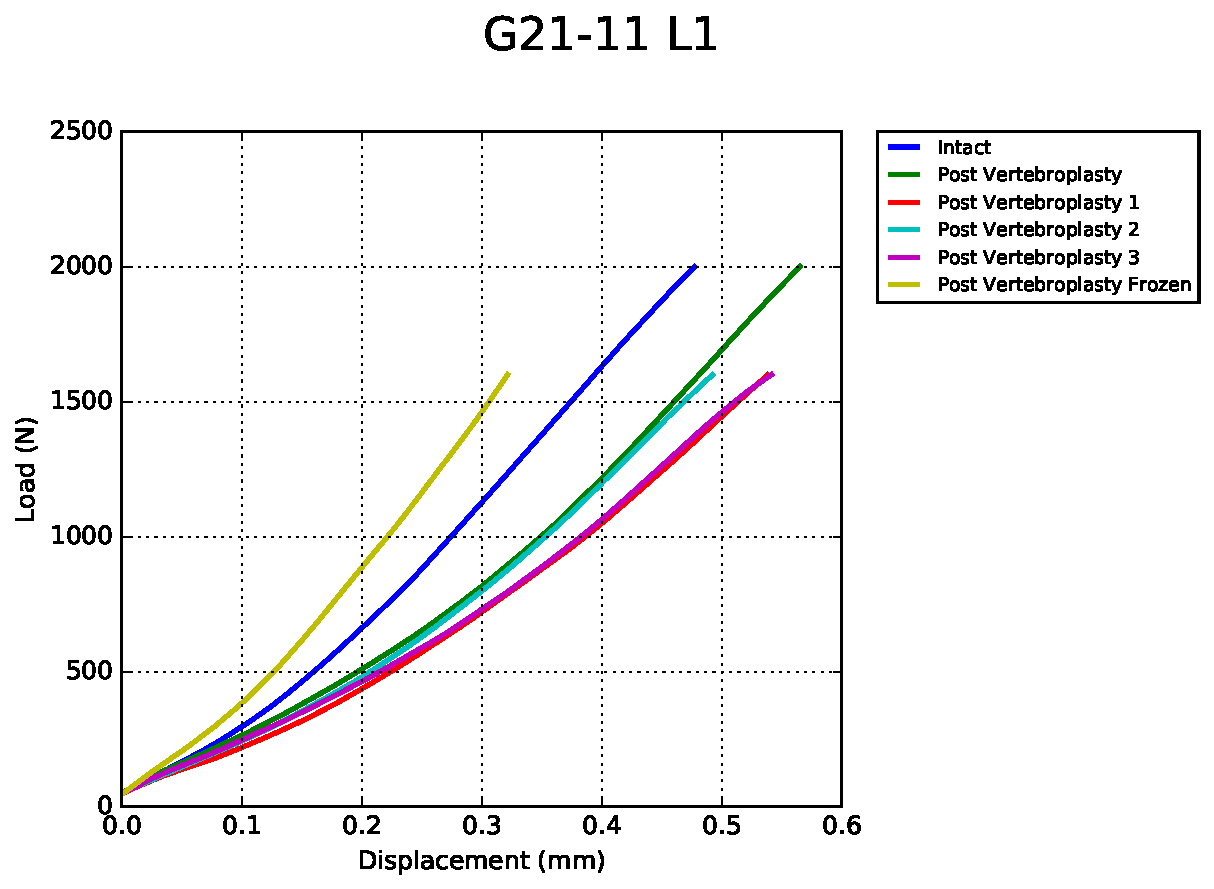
\includegraphics[width=4in]{Chapters/Chapter_HT_images/G21-11_L1.pdf}
  \caption{The load - displacement results for the Spine 3 L1 vertebra. Showing
    results of the intact load and post augmentation load up to 2000 N and the
    repeats and frozen load up to 1600 N.}
  \label{fig:Spine3_L1}
\end{figure}

\begin{figure}[ht!]
  \centering
  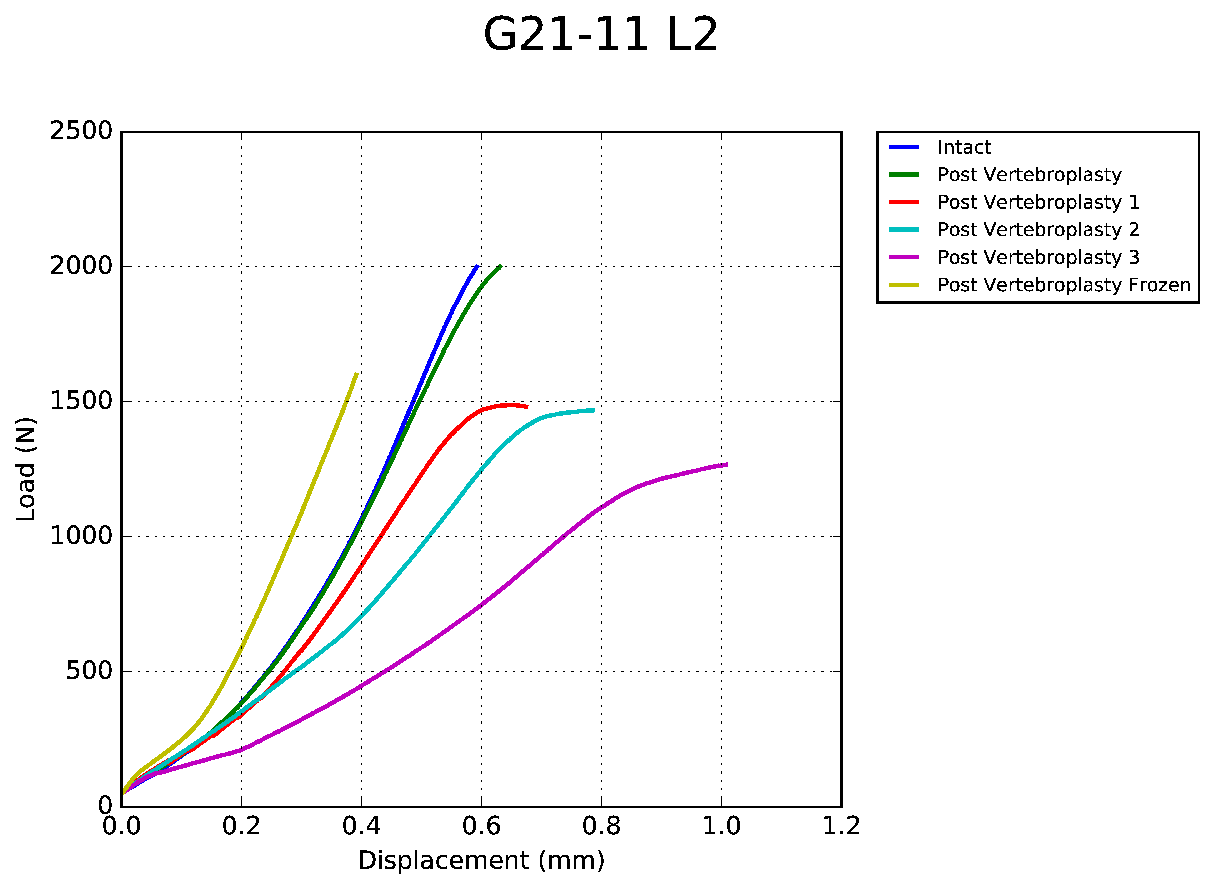
\includegraphics[width=4in]{Chapters/Chapter_HT_images/G21-11_L2.pdf}
  \caption{The load - displacement results for the Spine 3 L2 vertebra. Showing
    results of the intact load and post augmentation load up to 2000 N and the
    repeats and frozen load up to 1600 N.}
  \label{fig:Spine3_L2}
\end{figure}

\begin{figure}[ht!]
  \centering
  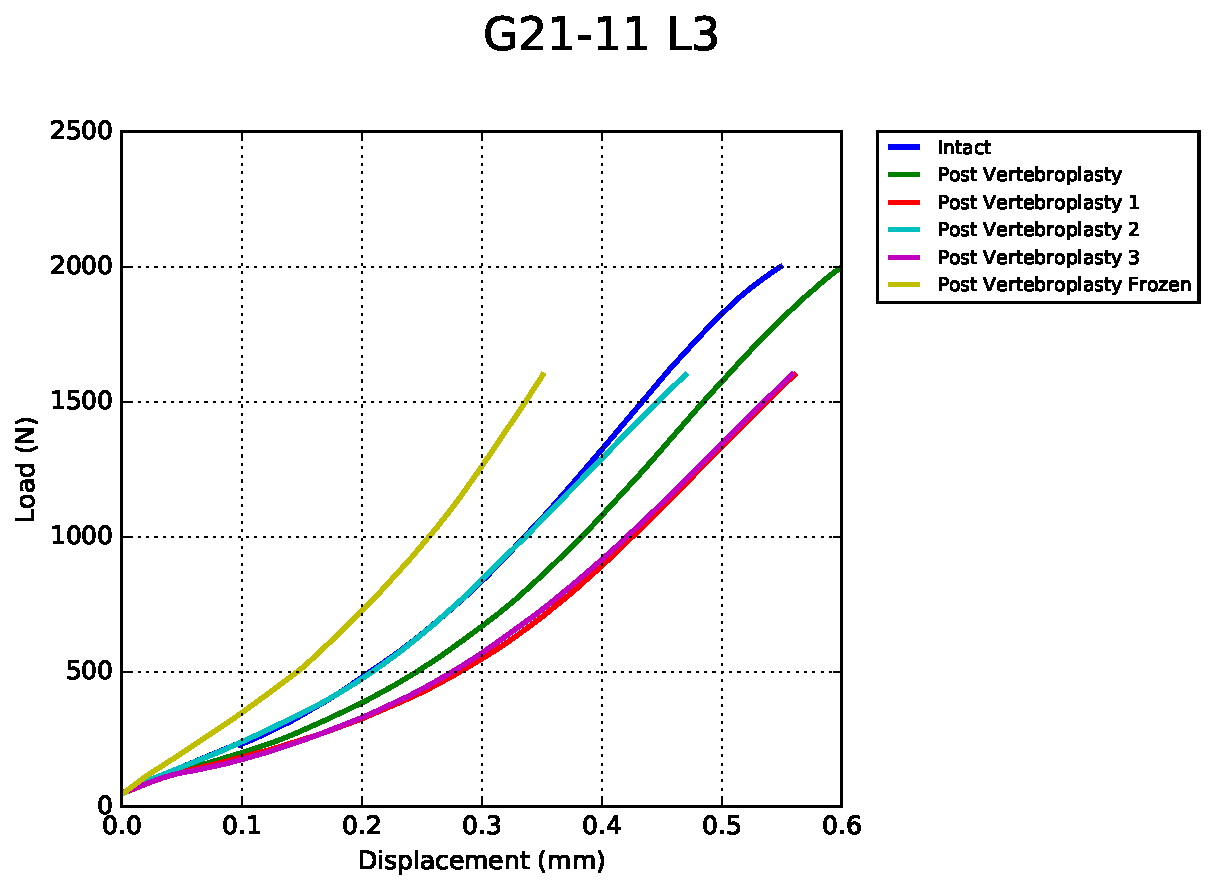
\includegraphics[width=4in]{Chapters/Chapter_HT_images/G21-11_L3.pdf}
  \caption{The load - displacement results for the Spine 3 L3 vertebra. Showing
    results of the intact load and post augmentation load up to 2000 N and the
    repeats and frozen load up to 1600 N.}
  \label{fig:Spine3_L3}
\end{figure}






\subsection{Vertebroplasty}

Despite the development of methods for the augmentation of bovine tail
vertebrae, the methods for augmenting human vertebrae were altered due to the
different geometry and density. The human vertebrae, being much less dense, did
not require the vertebroplasty needle to be inserted with the aid of a mallet.
Instead the needle could be pushed by hand through the cortical shell and into
the vertebral body.

An additional difference was the approach with the needle, instead of entering
the vertebrae through their pedicles an oblique approach was adopted. This was
due to variation in pedicle diameter between the L1 - L5 lumbar levels and
therefore the potential to damage the region and its load sharing capabilities.
The oblique approach therefore avoided creating this damage to the pedicle-canal
region, especially for the vertebrae with narrower pedicles and instead created
much less damage to the vertebral body.
An illustration of this approach can be seen in \cref{fig:vp-ill} with an example $\mu$CT scan shown in \cref{fig:vp-ill_scan}.


\begin{figure}[h!]
  \centering
  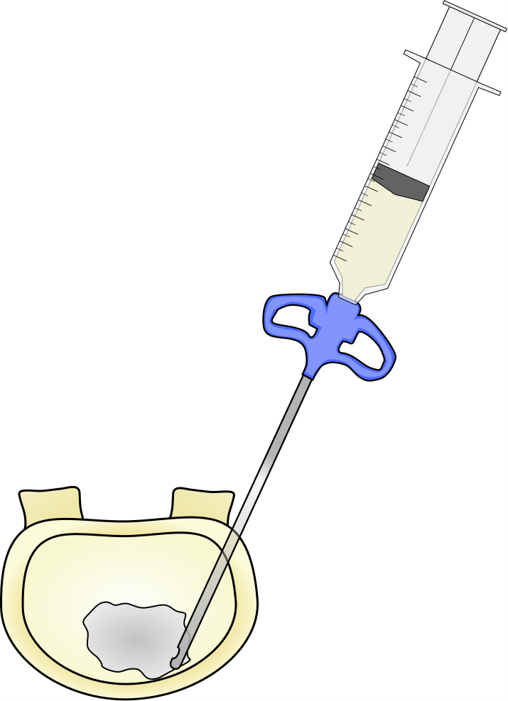
\includegraphics[width=4in]{Chapters/Chapter_HT_images/vp_illustration.png}
  \caption{An illustration showing the approach to needle insertion and cement position.}
  \label{fig:vp-ill}
\end{figure}


\begin{figure}[h!]
  \centering
  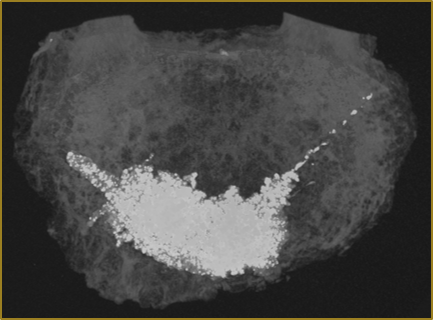
\includegraphics[width=4in]{Chapters/Chapter_HT_images/vp_illustration_scan.png}
  \caption{A $\mu$CT scan showing the injected volume of cement at the anterior of the vertebral body with the cement track from the exiting needle to the right. For this specimen cement leaked through the anterior wall, limiting the quantity of cement injected.}
  \label{fig:vp-ill_scan}
\end{figure}

A final difference to the needle insertion methods was a change to the needle.
Here, a side opening needle was used, allowing the cement to be directed into
the anterior-centre region of the vertebral body as opposed to directly out of
the needle end.

It was attempted to inject the largest possible volumes of cement into the vertebrae, mimicking the clinical process.
Like the clinical procedure the injection was stopped upon cement leakage, which generally occurred through one of the vascular channels at either the posterior or anterior portions of the vertebrae.
However, despite stopping the injection upon cement leakage through vascular channels leading from the vertebral body surface inwards, cement loss occurred.
In addition to this, cement was also lost in the needle itself, where as the cement set the amount of cement remaining in the needle became difficult to measure.
This meant that the cement fill could not be measured though the amount of PMMA leaving the syringe due to leakage and needle losses.
Hence cement fill volume was measured using segmented $\mu$CT scans, the methodology of which is described below.

\subsection{Vertebrae Characteristics}

Identifying the different characteristics for the set of lumbar vertebrae has
importance in understanding trends and relationships between the experimental
and computational results. For example a larger degree of anisotropy and hence
more directionality aligned trabeculae would potentially give a more
experimentally stiff vertebra, despite otherwise similar characteristics. Given
that much of the vertebral characteristics depend on the trabecular structure it
is important to understand how this varies between specimens. Furthermore, any
calculations originating from a description of the trabecular structure require
a correct threshold to be applied to the $\mu$CT scan. This threshold describes
the limit of the trabecular bone and hence the start of either marrow or empty
space. To enable a fair comparison between vertebrae a region of interest was
selected from the vertebral body. Given the large variation in cortical shell
thickness, along with certain vertebrae containing large osteophytes and other
extra bone growth, the region of interest (ROI) was selected to be the largest
cylinder that could fit within the vertebral body while not capturing any of the
cortical shell.

\subsubsection{Histograms}

In order to understand the spread of brightness' from the set of lumbar the
histograms of the ROIs were plotted (\cref{fig:normalisedhistogram}).

\begin{figure}[ht!]
  \centering
  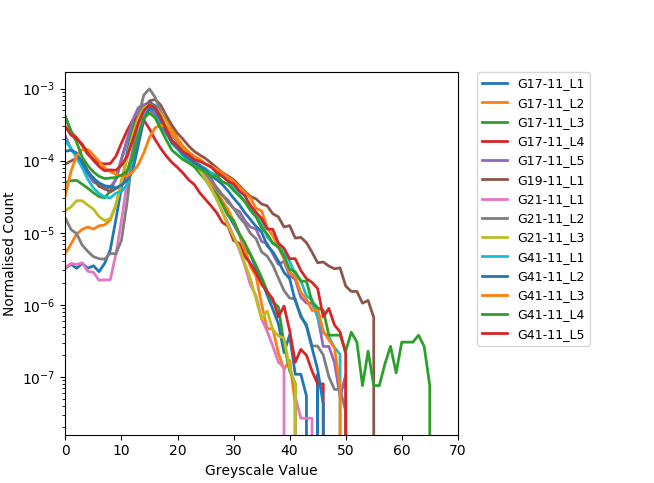
\includegraphics[width=4in]{Chapters/Chapter_HT_images/Normalised_Histogram.png}
  \caption{The normalised (with respect to the volume of the ROI) histogram data
    for the 14 lumbar vertebrae.}
  \label{fig:normalisedhistogram}
\end{figure}

The lower greyscale values represent the empty space within the ROI which
translates to regions where the bone marrow has exited the region, most likely
during the freeze thaw cycles. The peak in the histogram at an approximate
greyscale value of 16 is due to the bone marrow. The remaining portion of the
histogram represents bone, where variation is due to the differences in the
mineral content of the bone, with more mineralised bone appearing brighter on
$\mu$CT scans. The specimens ROIs that contain the brighter values are those
that contain osteophytes that contain more dense bone than the other cortical
shell, for example Spine 2 L1.

\subsubsection{Threshold Optimisation}\label{th_opt}


The full resolution scan is imported into imageJ where the threshold optimisation is carried out.
The BoneJ plugin for imageJ is used for all of the trabecular structure metrics, with the optimise threshold tool being the focus here.
The threshold optimisation feature works by optimising the connectivity (Conn.D) against threshold value \autocite{Doubea2010}.
This tool is run on the region of interest using the default settings for the connectivity options seen in \cref{tab:bonej}.
This chooses a threshold based on the peak in a connectivity against threshold plot and reports that value.
These values can be seen in \cref{tab:optTH}, showing considerable across the range of vertebrae.
However, the differences in these suggested thresholds can grouped with the spine, for example: the G17 spine has a range between 15 to 17, while the G41 spine has a range between 18 to 20.
This promotes the idea that these differences are due to the bone mineralisation of the bone, especially given that the G17 spine is from a Female and G41 from a male.

However, given that the chosen value for the threshold will directly impact the reported metrics, a consistent value was chosen of 18. Using lower or higher values for the threshold usually results in the trabeculae being described as thicker or thinner respectively.
Hence, the difference in the mineralisation between specimens will still be captured when using a fixed threshold, given that the binary image will be down sampled before material properties are acquired.
The results in \cref{tab:bv_tv_anis} show the BV / TV data and degree of anisotropy values for the 14 specimens using the fixed threshold of 18.
Similar trends to what could be seen from the optimise threshold results can be seen in the BV/TV data, with grouping between the
spines evident.
The Spine 1 spine has a much lower bone volume fraction compared to the other spines, which suggests a more osteoporotic spine, most likely resulting in less stiff vertebra.

\begin{table}[ht!]
	\caption{Settings used for the ImageJ plugin, BoneJ: Optimise Threshold.}
	\label{tab:bonej}
	\centering
	\begin{tabular}{c|c}
    Options & Values \\
    \hline
    \hline
    Tests & 11  \\
    Range & 0.2 \\
    Subvolume Size & 256 \\
    Erosian Cycles & 0 \\
    Dilation Cycles & 0 \\
    \hline
	\end{tabular}
\end{table}

\begin{table}[ht!]
	\caption{The suggested threshold from the optimise threshold BoneJ tool for the 14 lumbar vertebrae in the set.}
	\label{tab:optTH}
	\centering
	\begin{tabular}{c|c}
    Specimen    & Suggested Threshold   \\ \hline \hline
    Spine 1 L1 & 17 \\
    Spine 1 L2 & 16\\
    Spine 1 L3 & 16\\
    Spine 1 L4 & 15\\
    Spine 1 L5 & 16\\
    Spine 2 L1 & 23\\
    Spine 3 L1 & 18\\
    Spine 3 L2 & 19\\
    Spine 3 L3 & 19\\
    Spine 4 L1 & 20\\
    Spine 4 L2 & 19\\
    Spine 4 L3 & 18\\
    Spine 4 L4 & 19\\
    Spine 4 L5 & 18\\
    \hline
	\end{tabular}
\end{table}



\section{Computational Methods}

The split between different modelling methods, computational and experimental is not terribly clear, given that computational methods are employed in the scanning and material property analysis described above.
However, the methods described in this section describe the process used to model non-augmented and augmented vertebrae, with associated sensitivity tests to understand the most appropriate approach to various aspects of the modelling process.




\subsection{Non-augmented Vertebrae Modelling Sensitivity Tests}\label{sec:non_aug_sens}

Given the aims of the project - to include the models generated here into a
larger set of vertebral models for use in statistical shape modelling, it is
useful to model the vertebrae in a scanner independent method. A method for
doing this (BV/TV modelling method) uses a full resolution scan with the bone
regions segmented using a threshold. This full resolution segmented scan is then
downsampled to voxels with edge length of 1 mm, meaning that each voxel has a
greyscale value proportional to the BV/TV value for the region captured by that
voxel. Areas that contain more bone will therefore have a higher greyscale
value. This method is purely dependant on the threshold selected defining the
bone and hence, given that threshold values can be repeatedly and correctly
selected with the methods shown in Section~\ref{th_opt}, it is scanner independent.

Other sensitivity studies present difficulties due to the models reliance on the underlying greyscale background.
This is due to the greyscale optimisation process required to obtain a new conversion factor between the greyscale values and the Young's modulus for every change made to the material properties or boundary conditions of the models.
This is in order to understand the effect the change has on the agreement between experimental and computational results, and because a change to the material properties or boundary conditions may not have a systematic or uniform effect on the results.
Due to this, simple sensitivity tests become difficult, including common convergence studies.

\subsubsection{BV/TV Modelling Method}\label{bvtv_method}

This method gives the opportunity to keep much of the detail that is often lost when downsampling image data.
Specifically, the method described gives the vertebral models much more definition of the cortical shell and internal trabecular structure while maintaining the 1 mm cubed resolution and the computational cost benefits associated with that.
The method follows that found in a study by Robson Brown et al.
\cite{RobsonBrown2014} with a few minor changes. The scans are converted from the ScanCo proprietary ISQ format into a stack of TIFF files using an in house Matlab script, which in additionally reduces reduces the 16 bit data to 8 bit images.

The set of vertebral specimens were split at this stage into two sets, allowing
an understanding of how the bone volume fraction method affects the results compared to the method described in Section~\ref{finite-element-modelling-methods}.
To the set using the bone volume fraction method a threshold was applied at the full 82 $\mu$m resolution.
This threshold was chosen to be a greyscale value of 18, the mean of the values described in section Section~\ref{th_opt} and was applied to the scan stacks in imageJ.
Once the binary stack was created a Gaussian filter was applied, also within imageJ, with $
\sigma_{x,y,z} = 1 $.
This was applied in order to remove speckling found surrounding the end-caps and some of the other noise visible in the scans.
The two stacks of images are then imported into ScanIP; carried
out by opening one stack of images (the original stack) and then importing a
second background (the binary image stack). Both backgrounds are downsampled to
voxel sizes of 1 mm$^3$, with the (originally) binary stack being used to create
the mask for the vertebrae and the original stack being used for the end-caps.
Greyscale material properties for the vertebral mask are taken from the binary
stack, while the remainder of the methods follow the same process as the
original method.
A comparison of the two approaches can be seen in \cref{fig:normal_vs_bv_tv_seg}, where the improved definition of trabecular structure and cortical shell using the bone volume fraction method can be seen in E and F.

\begin{figure}[ht!]
\centering
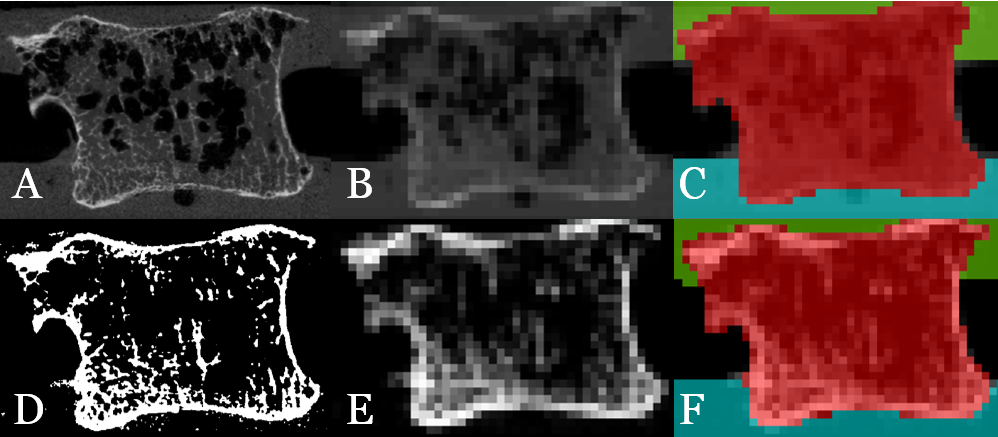
\includegraphics[width=.65\textwidth]{Chapters/Chapter_HT_images/normal_vs_bvtv_seg.png}
	\caption{A comparison of the normal method (A, B and C) and the bone volume fraction method (D, E and F). A shows the full (82 $\mu$m) resolution scan, B shows the same image downsampled to 1 mm resolution and C shows the segmented scan. D shows the segmented bone at 82 $\mu$m, E shows this image downsampled to 1 mm and F shows this image after segmentation.}
\label{fig:normal_vs_bv_tv_seg}
\end{figure}

%\begin{figure}[ht!]
%  \centering
%  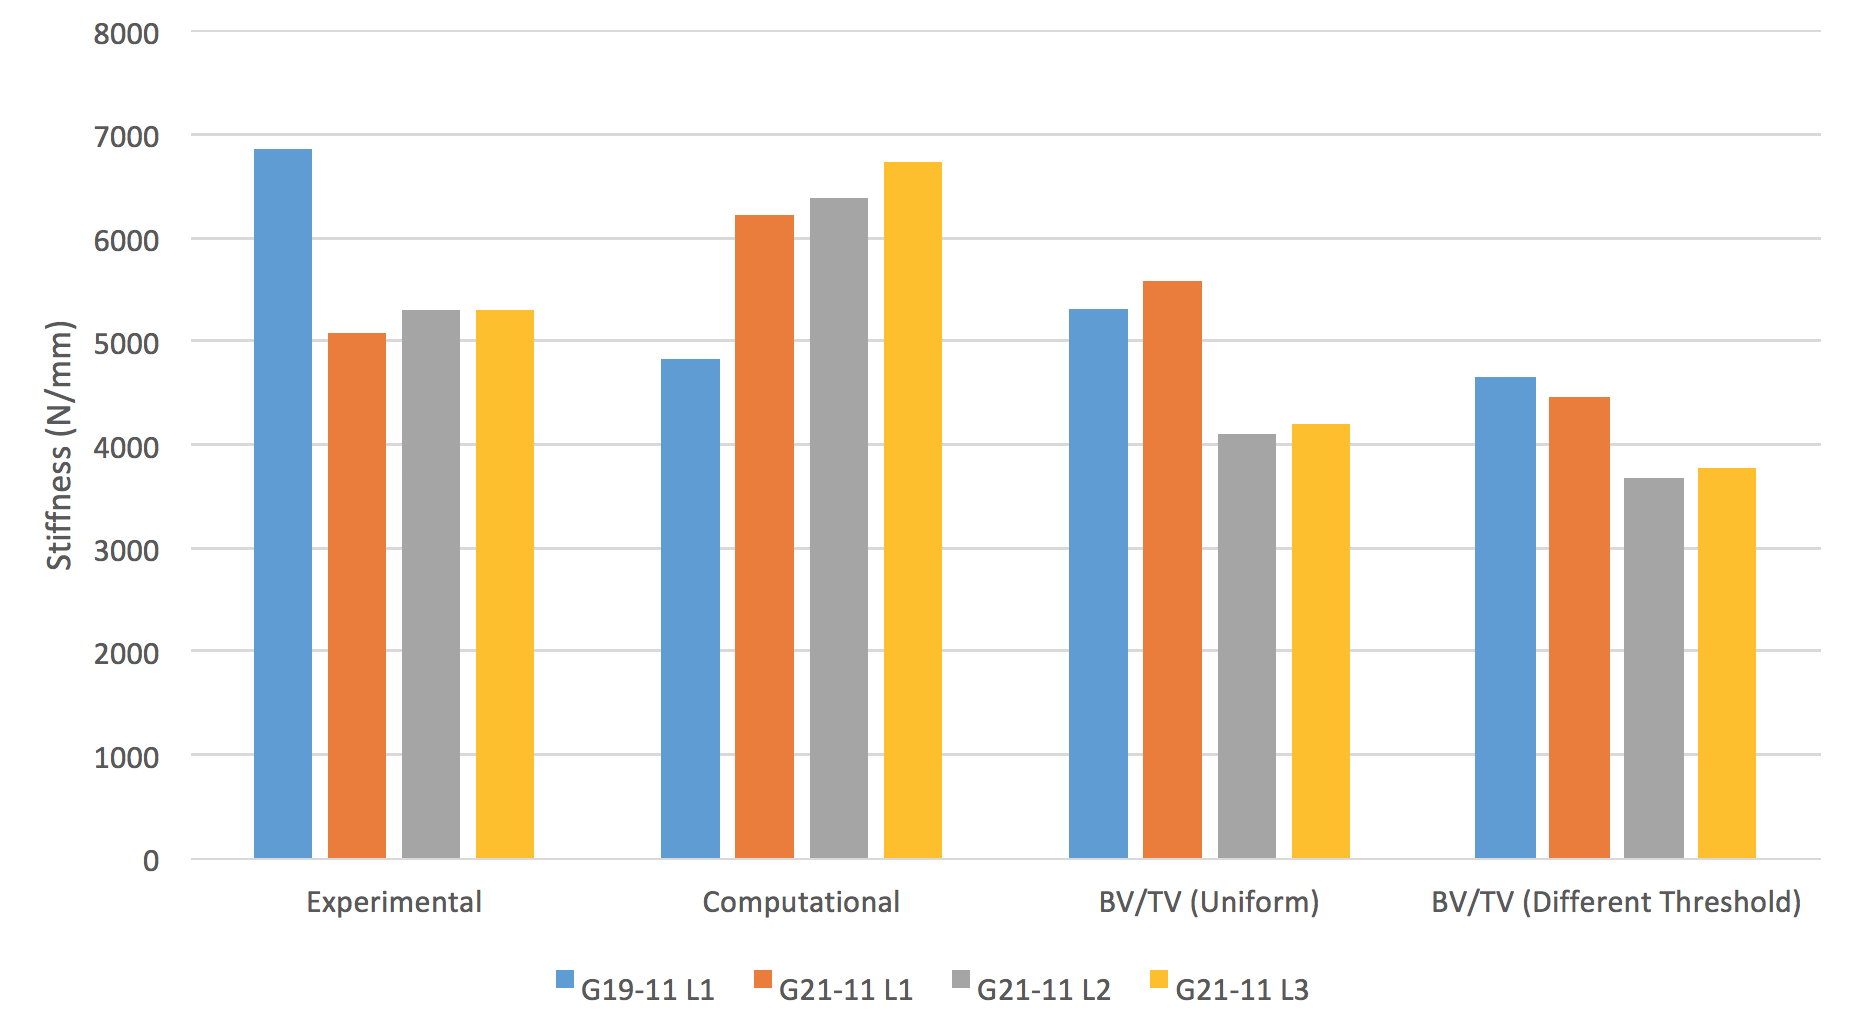
\includegraphics[width=6in]{Chapters/Chapter_HT_images/diffModellingMethods.png}
%  \caption{The stiffness results of three different FE methods for four intact
%    human vertebrae compared to the experimental stiffness results. Interest
%    should be drawn to the ratio between specimen models rather than the values
%    themselves, given that the conversion factors between greyscale values and
%    Young's modulus have not been optimised at this stage. Results show the
%    difference between the currently used method of modelling the vertebrae and
%    the BV/TV based methods (both with uniform thresholds and different
%    thresholds for each specimen).}
%  \label{fig:diffModellingMethods}
%\end{figure}




%\subsubsection{Predicting Vertebral Yield Point}\label{predYield}

\subsubsection{Load Position Sensitivity}

In order to understand how the vertebrae respond to different loading positions, 16 different positions were tested, shown in \cref{fig:loading_pos}.
These positions included 1~mm and 2~mm aways from the centre in the posterior, anterior, left and right directions along with larger deviations of 10~mm and 20~mm from the centre in the same directions.
The same boundary conditions, along with the 1 mm of displacement described above were applied to the different loading positions and the change in stiffness was recorded.

\begin{figure}[ht!]
\centering
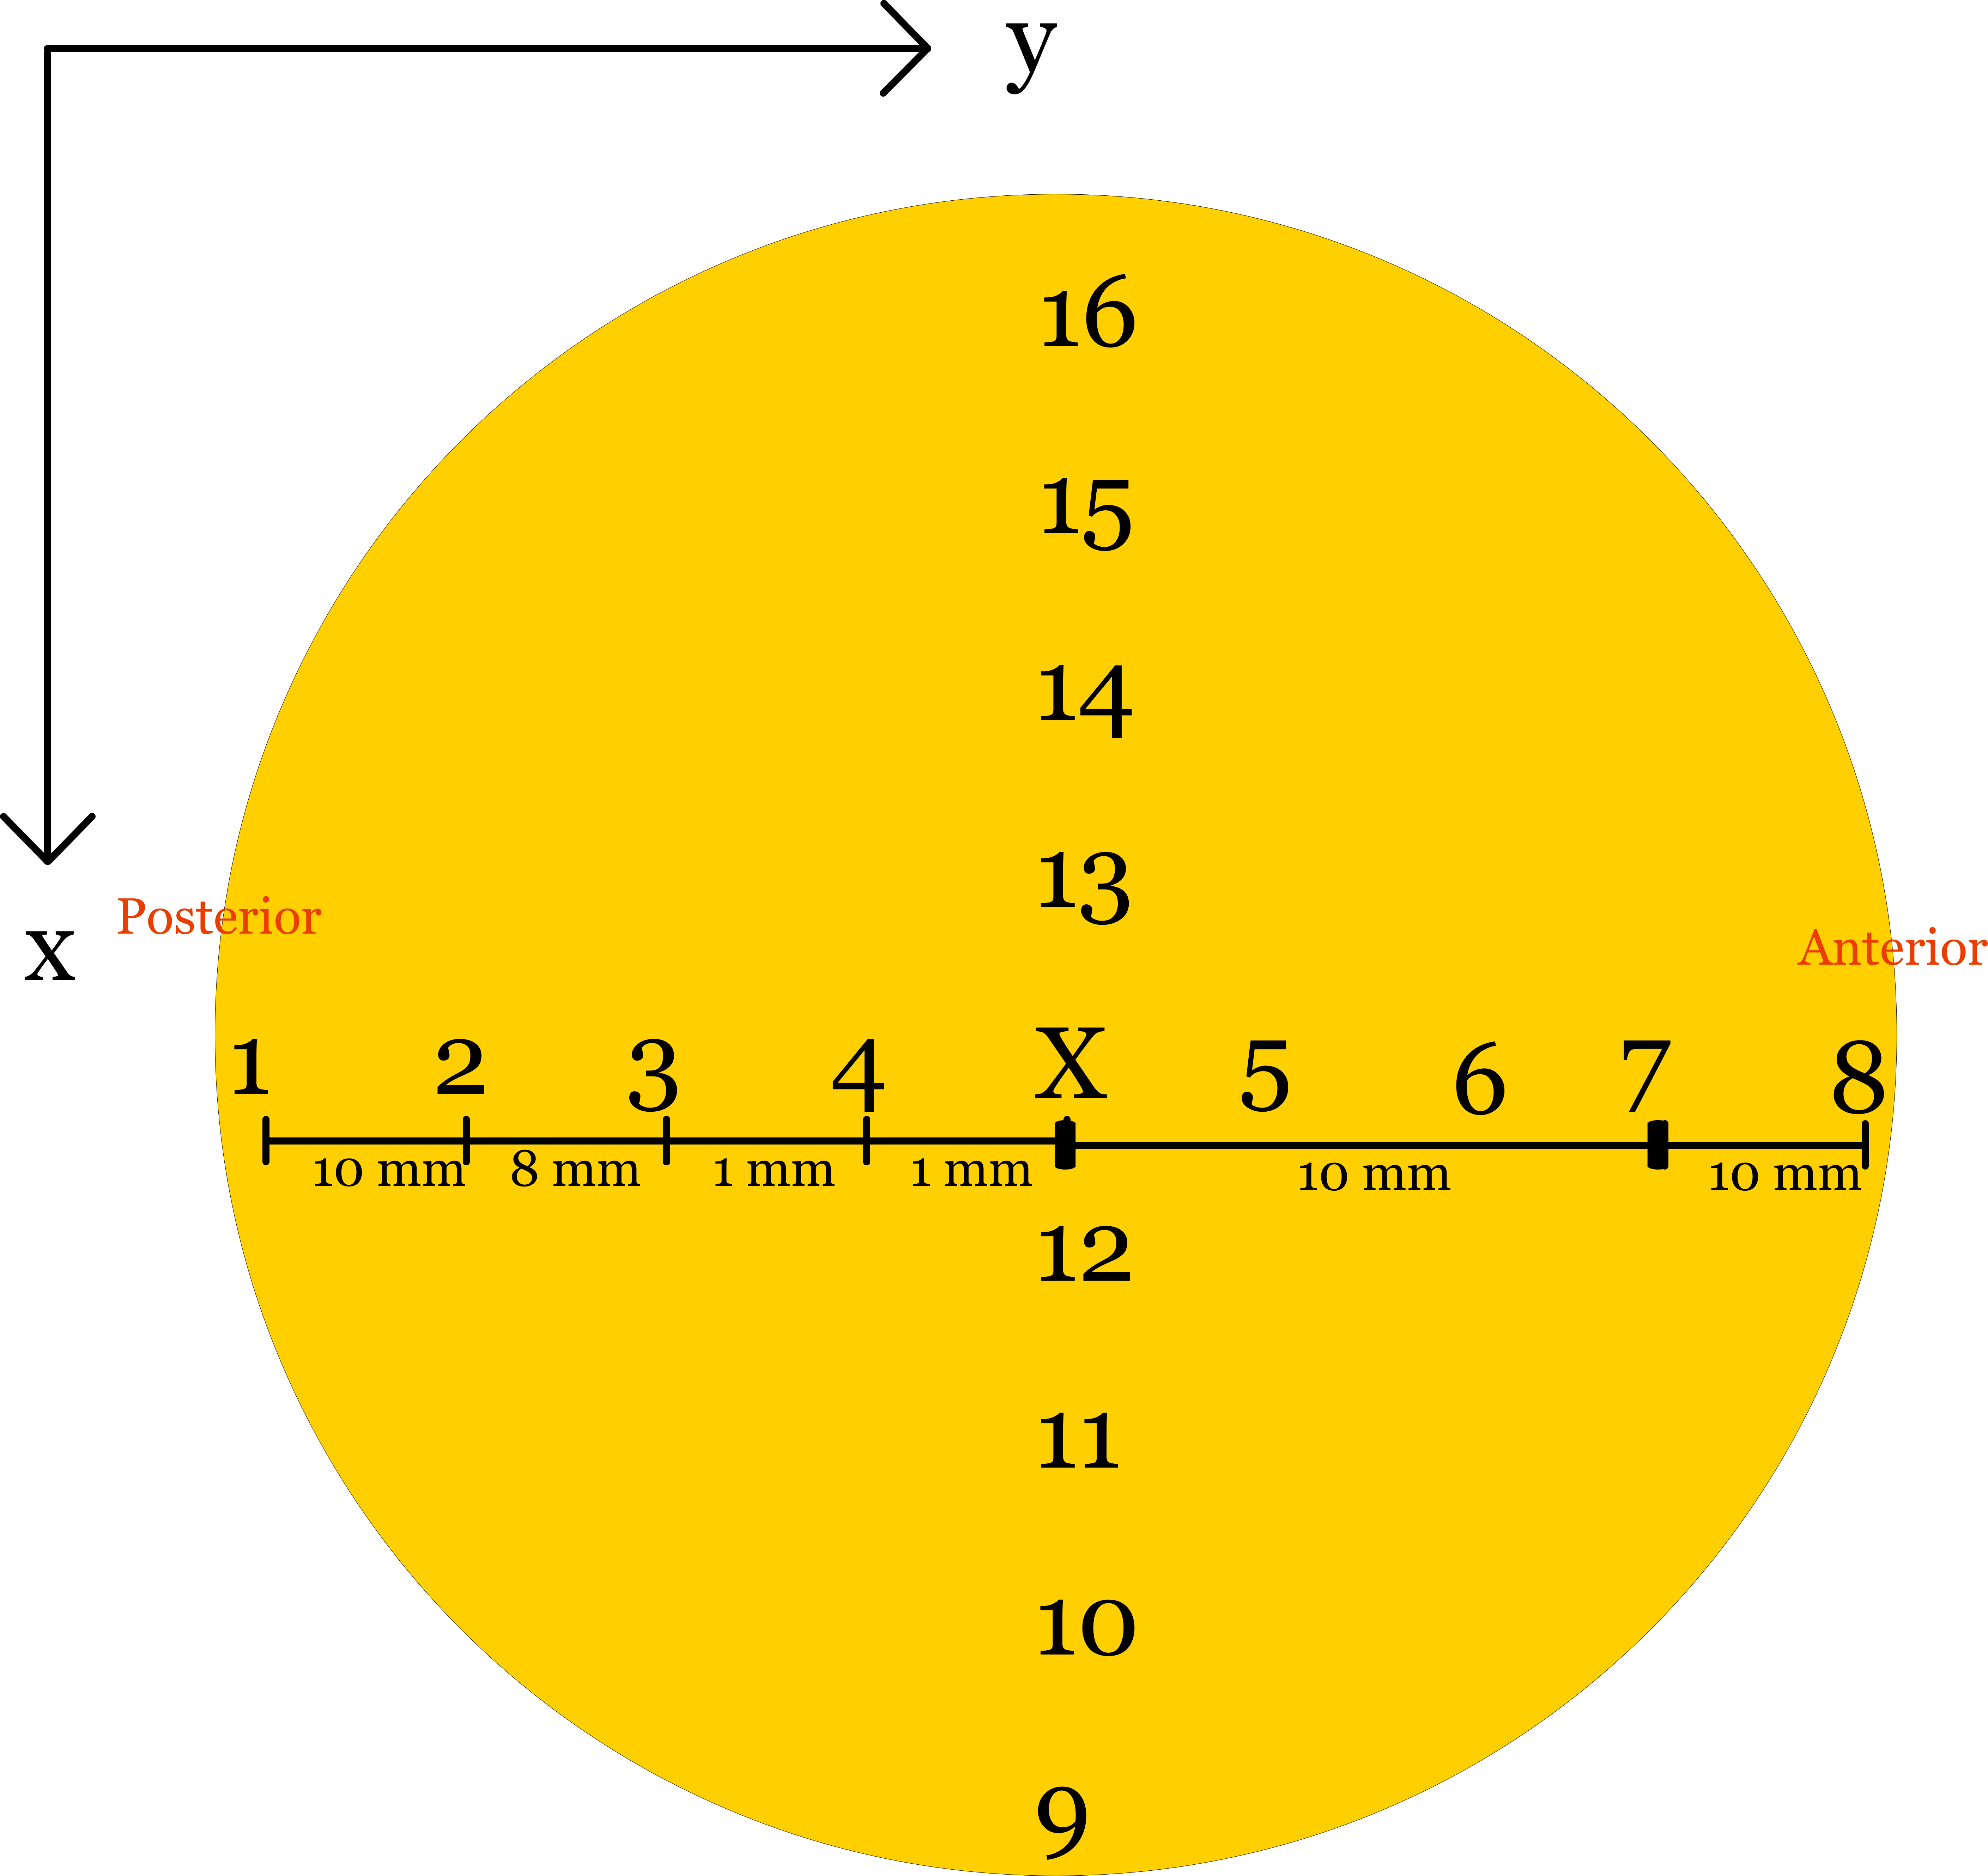
\includegraphics[width=.7\textwidth]{Chapters/Chapter_HT_images/Loading_positions_Human.png}
\caption{The loading positions used for the load variation tests. Position X is the original central loading position for ap and lr loading, other loading positions are 1~mm, 2~mm, 10~mm and 20~mm away from the centre.}
\label{fig:loading_pos}
\end{figure}


The results of the load position sensitivity tests (\cref{fig:hum_load_ap}) show that on average, small posterior loads (above denser bone) result in higher stiffness's while all anterior loads result in a reduced stiffness. Loads lateral to the central loading point (\cref{fig:hum_load_lr}) resulted in little mean change to the stiffness of the models for the 1 and 2~mm positions.
Larger movements away from the central loading position (10~mm and 20~mm) result in almost all vertebrae presenting a reduction in stiffness.
Loading positions at 20~mm left and right present the largest reductions, where in the body the expected loads are less compared to anterior/posterior loading.
Additionally, larger anterior loads resulted in larger reductions in the stiffness, given the less dense nature of anterior portions of the vertebral body

It also shows that the effect of movements of 1 mm away from the experimental loading position only changes the stiffness by approximately 5 \%.
Given the resolution of the models is limited to 1 mm, the accuracy of the selection of the experimental loading positions is also limited to 1 mm.
The maximum 5 \% change to the stiffness when posterior or anterior may describe some of the error seen when comparing the experimental and computational results.

\begin{figure}[ht!]
\centering
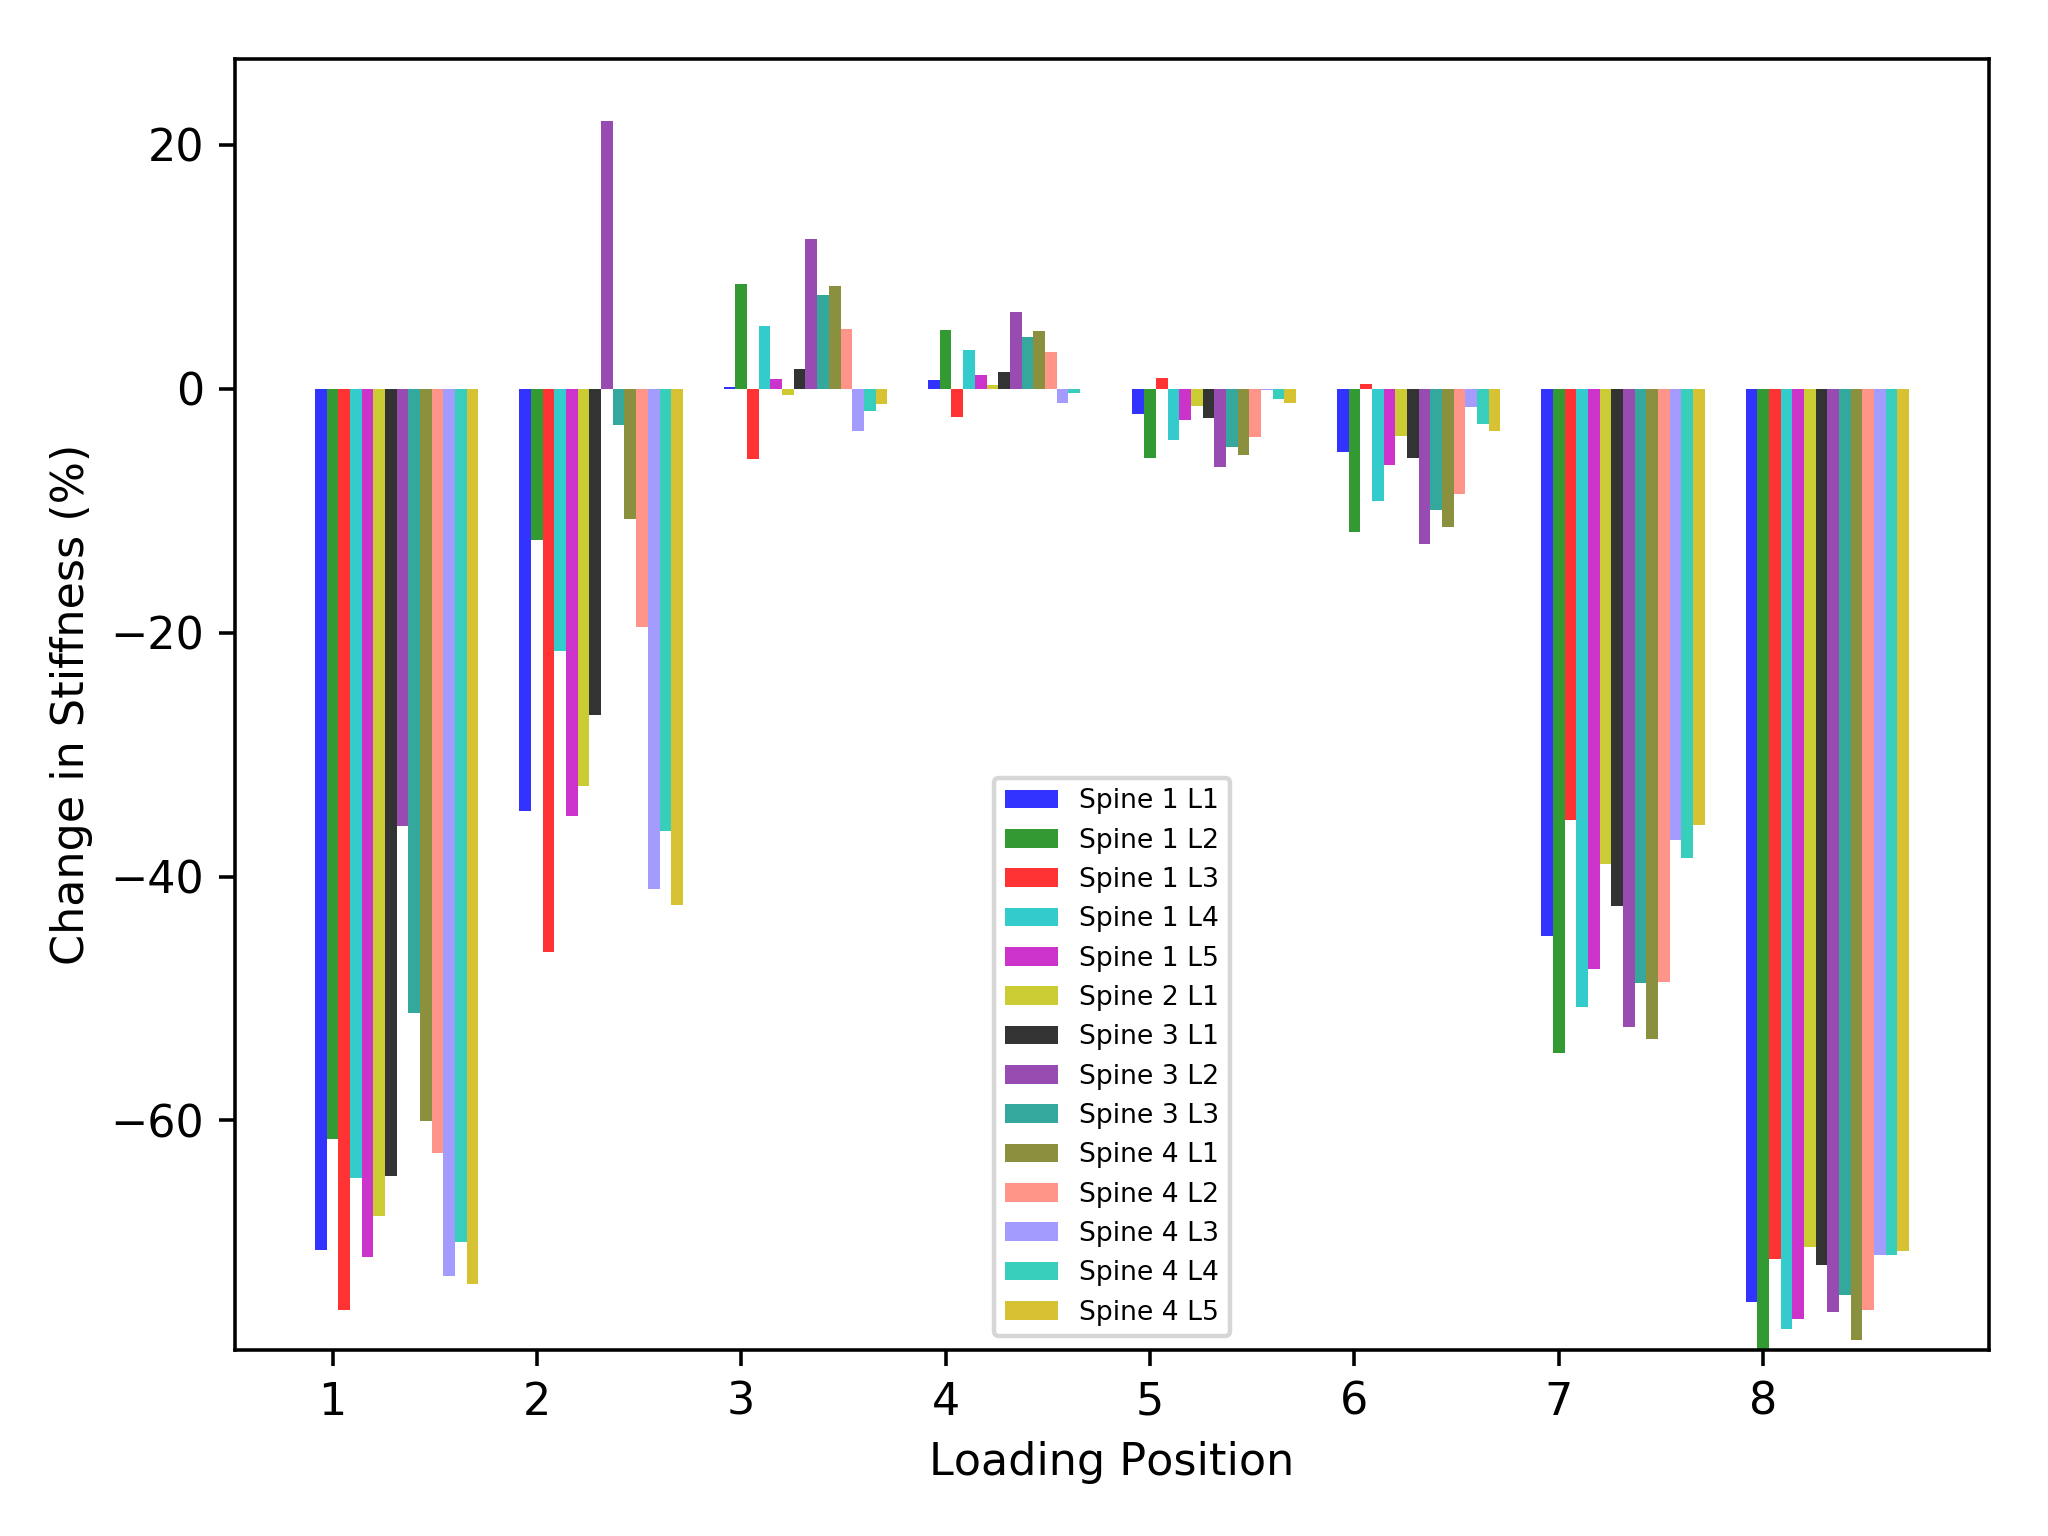
\includegraphics[width=\textwidth]{Chapters/Chapter_HT_images/hum_ap.png}
\caption{The effect of the loading position for the human lumbar vertebrae, shown as a percentage change compared to a central loading position, for load positions from the posterior to anterior according to \cref{fig:loading_pos}}
\label{fig:hum_load_ap}
\end{figure}

\begin{figure}[ht!]
\centering
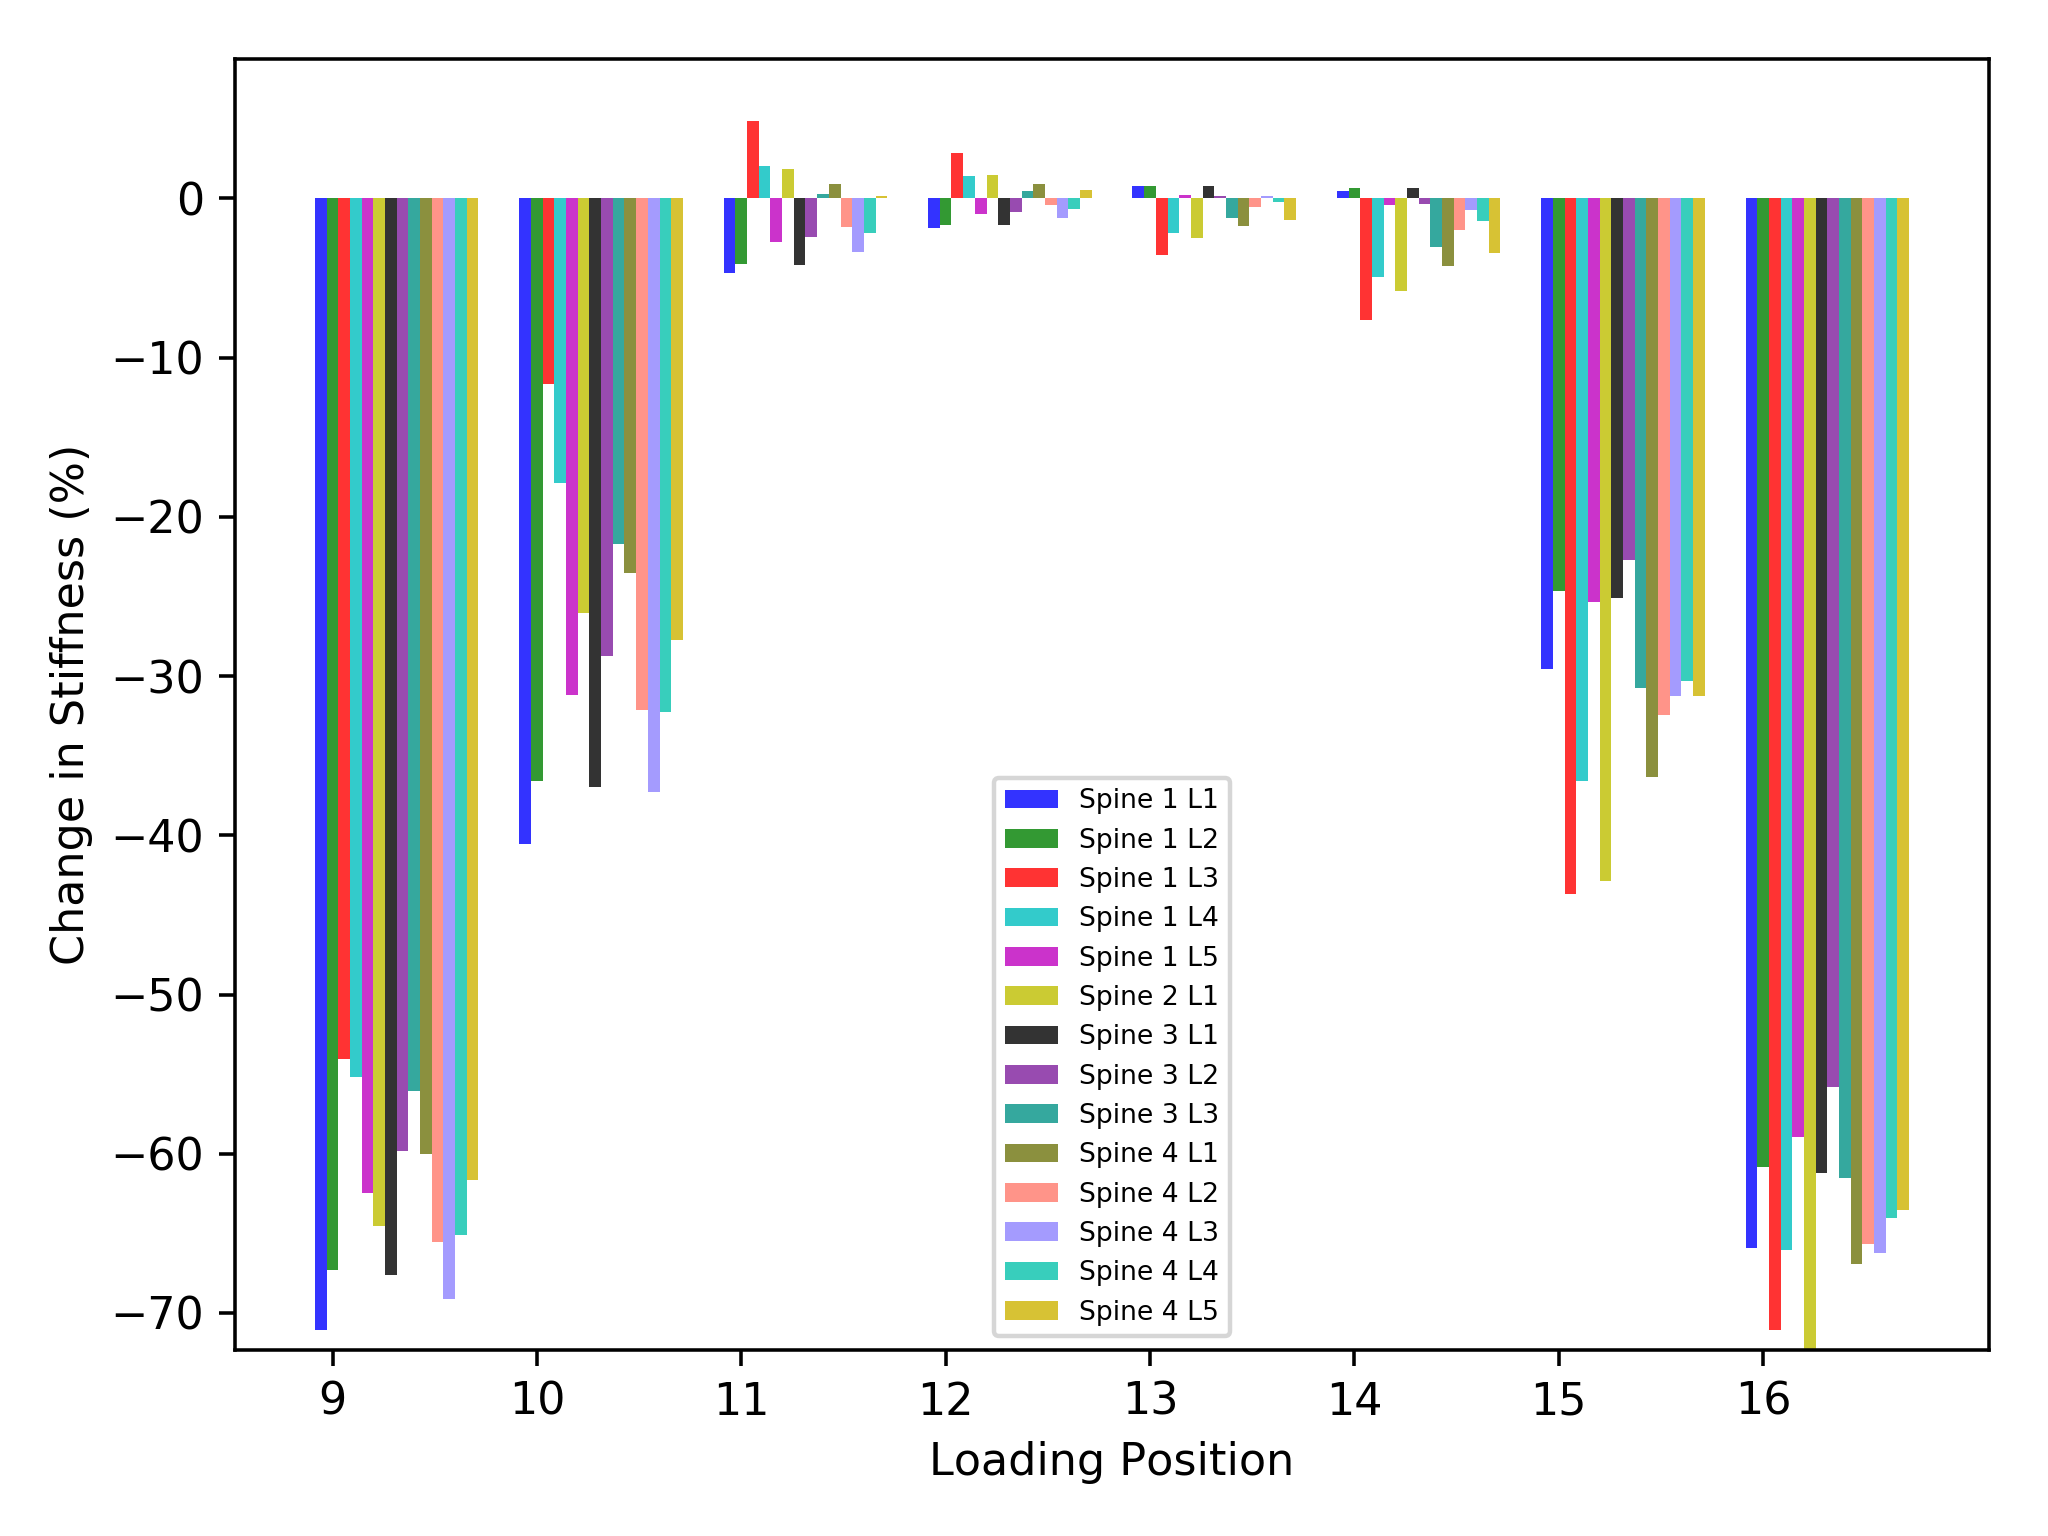
\includegraphics[width=\textwidth]{Chapters/Chapter_HT_images/hum_lr.png}
\caption{The effect of the loading position for the human lumbar vertebrae, shown as a percentage change compared to a central loading position, for load positions from the left to the right according to \cref{fig:loading_pos}}
\label{fig:hum_load_lr}
\end{figure}



\subsubsection{End-cap Depth \& Contact sensitivity}

The stress distribution at the surface of the vertebral body shows high stress at the edges of the cement endcaps, at both the top and bottom of these regions, shown in \cref{fig:stress_lines}.
Experimentally the endcaps are merely moulded to the shape of the top and bottom of the vertebral body, however, previous work and other studies have used tied contact between the bone and endcaps, removing any motion between the two and locking neighbouring nodes together.
Additionally, the depth of these endcaps varies between 5 mm and 20 mm depending on the shape of the vertebral endplates.
The more concave the vertebral endcap was the more cement was required to fill the space forming a flat cement surface.

\begin{figure}[h!]
\centering
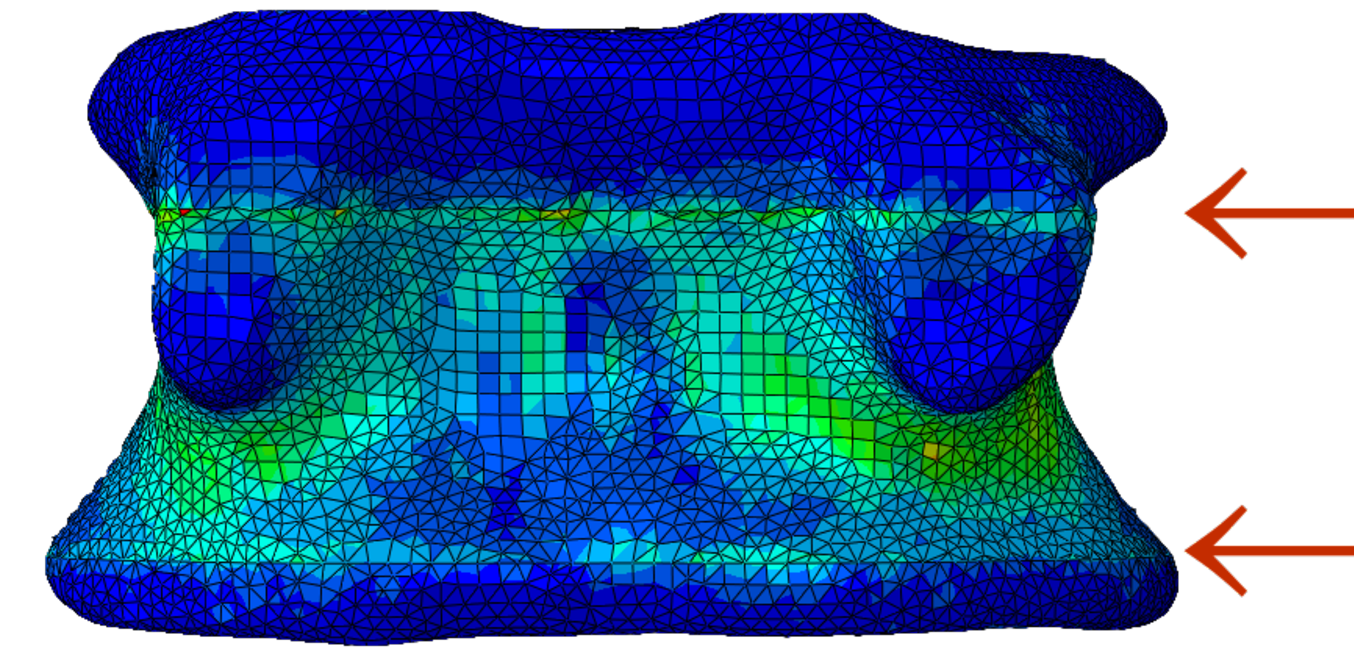
\includegraphics[width=.65\textwidth]{Chapters/Chapter_HT_images/stress_lines.pdf}
\caption{The effect of having tied contacts between the endcaps and the bone, with the increases in Von Mices stress indicated.}
\label{fig:stress_lines}
\end{figure}


Given this variation, tests identifying the effect of changing the endcap depth were carried out using FEA models with different depths of $\pm$ 1, $\pm$ 2 and $\pm$ 3 mm for the top and bottom endcaps independently and together.
Additionally, different interactions between the bone and cement endcaps were tested.
This included the current standard method of a tied interaction and replacing this with a frictionless contact between the two materials.
Finally, the effect of changing the cement endcap depth with the frictionless contact was also investigated, along with variations to the properties of the frictionless contacts.
This was carried out given that, experimentally, there is no tied contact between the PMMA and the bone due to the lack of adhesive properties for the PMMA.

The endcap depth was altered by adding and removing layers within the model file in ScanIP, re-meshing the model and running the files using the same Abaqus python scripts.
Endcap contacts were changed within the Abaqus python scripts, by firstly removing the ties between the endcap and the vertebra.
An interaction property was created with tangential behaviour set to frictionless and normal behavior with properties: $pressureOverclosure=HARD,  constraintEnforcementMethod=Default$ and the final option was experimented with, $allowSeperation=ON/OFF$.
The $allowSeperation$ variable determines whether separation is permitted once contact is established and models ran correctly with it set to its default of $ON$.
However, when experimenting with the effect of loading position, especially with loads applied far from the vertebral centre, the solver struggled to converge.
Disallowing separation after contact was shown to have a small effect on the results (the outputted stiffness) and allowed the models to run to the completion of the job.
The remaining settings were set to the default for a generic contact: 

$
	initialClearance=OMIT \\
	adjustMethod=None \\
	sliding=SMALL \\
	enforcement=NODE\_TO\_SURFACE \\
	thickness=ON \\
	supplementaryContact=SELECTIVE \\
	interactionProperty=contactName \\
	smooth=0.2 \\
	bondingSet=None \\
$

The results shown in \cref{fig:with,fig:without} show that regardless of the contact, increasing the depth of the endcaps significantly increases the stiffness of the vertebrae, while reducing the depth reduces the measured stiffness.
The effect this extra or reduced constraint caused by the changing endcap depth broadly follows the same trends for the two vertebrae tested.
However, the response does differ most notably at the extremes of endcap depths ($\pm$3 mm), where the spine 4 L5 vertebrae experiences the greater reduction in stiffness when reducing the endcap depth, while the spine 1 L2 vertebrae sees the greater increase following depth increases.
This difference is a consequence of the differences in the density of the vertebrae (where spine 4 is, on average, much denser than spine 1 in terms of mean greyscale value) and the differences in the shape (the L5 vertebrae being much wider with greater protruding bone spurs at the bottom of the vertebrae and the narrower L2 vertebrae having the bone spurs at the top of the vertebrae.
These shape differences can be seen in \cref{fig:Spine 1_projection,fig:Spine 4_projection}.

The variation in the change to the stiffness within $\pm$ 1mm change in depth was up to 5 \%, for both cases.
Given that the maximum error in masking the cement endcaps is 0.5 mm due to the resolution that is used for the segmentation, it suggests that this error has a minimal effect on the end results.

The effect of changing the contact from tied to frictionless can be seen by comparing \cref{fig:with,fig:without}.
Excluding the very large change in stiffness seen in the L5 vertebra when reducing the depth of the inferior endcap, the adoption of the frictionless contact between endcap and vertebrae means that the effect of endcap depth on measured stiffness is reduced.
This is due to a reduction in the constraining nature of the frictionless contact.
The anomalous L5 vertebrae here is a function of having less support and the slipping that this allowed, resulting in the reduced measured stiffness.
Optimising the greyscale conversion factor for the set of models with a tied constraint and a frictionless contact gave concordance correlation coefficients of 0.848 and 0.865 respectively.
Therefore the frictionless contact providing a small improvement in the agreement between the computational and experimental results.





\begin{figure}[h!]
\centering
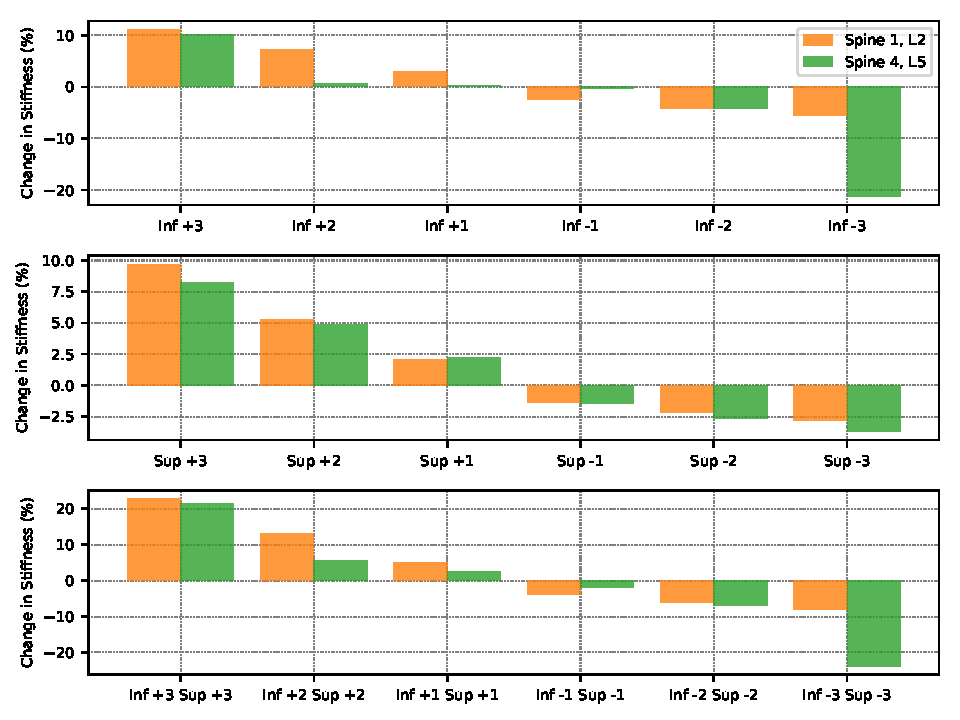
\includegraphics[width=\textwidth]{Chapters/Chapter_HT_images/with.pdf}
\caption{The percentage change in stiffness following a change to the endcap thickness. Inf and Sup show changes of $\pm$ 1, 2 and 3 mm to the inferior and superior endcap depth respectively. The endcaps have a tied contact to the vertebrae.}
\label{fig:with}
\end{figure}

\begin{figure}[h!]
\centering
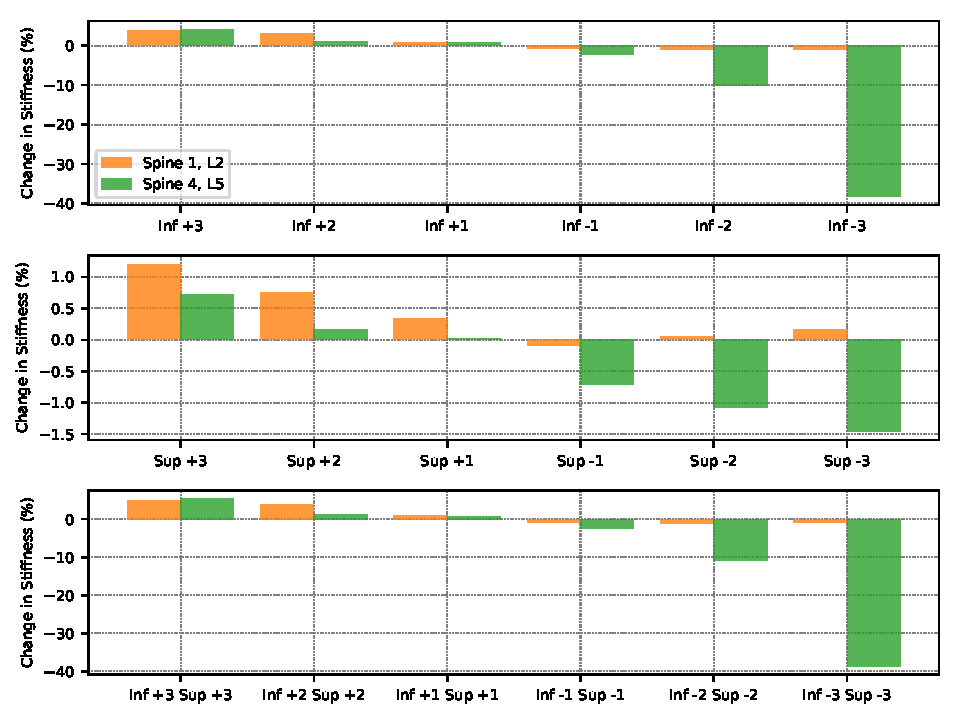
\includegraphics[width=\textwidth]{Chapters/Chapter_HT_images/without.pdf}
\caption{The percentage change in stiffness following a change to the endcap thickness. Inf and Sup show changes of $\pm$ 1, 2 and 3 mm to the inferior and superior endcap depth respectively. The endcaps have a frictionless contact to the vertebrae.}
\label{fig:without}
\end{figure}

Further tuning of the specifics of the frictionless contact could be carried out to see if an improved agreement could be achieved would be a simple addition to this sensitivity test.
However, due to the greyscale conversion factor optimisation process required to test each option this would be a timely operation, which, given the minimal effect of changing to the frictionless contact, could yield negligible results.




\subsection{Material Properties}

The general method for getting material properties for the bone elements in the FE models uses the same approach as used in \cref{material-properties-bov} where the Young's modulus of each element is equal to the greyscale value multiplied by a conversion factor.
The conversion factor is optimised by comparing the computational stiffness against the experimentally acquired stiffness.
For the optimisation process the vertebrae were split into two groups at random, giving a calibration and validation set, allowing a test of the validity of the greyscale conversion factor.
The split of the vertebrae for these two sets can be seen in \cref{tab:calib_valid}.

\begin{table}[ht!]
	\caption{The vertebrae used for the calibration set and the validation set in the optimisation process.}
	\label{tab:calib_valid}
	\centering
	\begin{tabular}{c|c}
    Calibration Set   & Validation Set  \\ \hline \hline
    Spine 1 L4 & Spine 1 L1  \\
    Spine 1 L5 & Spine 1 L2\\
    Spine 2 L1 & Spine 1 L3 \\
    Spine 3 L2 & Spine 3 L1\\
    Spine 4 L1 & Spine 3 L3\\
    Spine 4 L2 & Spine 4 L3\\
    Spine 4 L4 & Spine 4 L5 \\
    \hline
	\end{tabular}
\end{table}


Results from the initial optimisation process using the calibration and validation processes gave good results, in that the agreement of the validation set had CCC values of above 0.5.
The validation set for the ``normal" method had a CCC value of 0.591 and the CCC value for the validate set from the ``bone volume fraction" method gave a value of 0.831.

Given the problems associated with calculating the greyscale conversion factor with various sensitivity tests described in \cref{sec:non_aug_sens}, the calibration and validation sets were only used for the initial test, once using the ``normal" method and once using the ``bone volume fraction" method.
This validated the use of the optimisation process while allowing more accurate greyscale conversion factors for the sensitivity tests and final values given that the input set of human vertebrae was relatively small.

Following the results of the sensitivity tests the final value from the optimisation process for the greyscale conversion factor was 0.0009625.
This was used for the bone properties for all final non-augmented models and augmented models.

The remaining material properties used for all of the models are a Poisson's ration of 0.3 for the bone and endcaps and a Young's modulus of 2.45~GPa for the endcaps. 

\subsection{Modelling Augmentation}

Given the limited validation of models achieved using bovine tail vertebrae (due to the reasons discussed in Section~\ref{bov:results}), a range of different material properties and approaches to modelling the bone-cement interface were investigated.
In addition to varying the material properties of the injected volumes of cement, the effect of using a combination of scans from before and after augmentation has been experimented with.
To achieve this scans of pre/post augmentation were registered.
This method utilised the BV/TV method described earlier, where the non-augmented full resolution thresholded scan is registered to the full resolution augmented scan.

\subsubsection{Registration of $\mu$CT Scans}

Artificial brightening of regions surrounding the internal cement (specifically the concentrated volumes of barium sulphate and the artefacts associated) affect the material properties that are applied to the material, seen in the right-hand image in \cref{fig:reg_demo}.
To bypass this effect the two models, intact and post-augmentation models can be registered - translating them into the same spacial location.
This allows the cement to be defined, masked and modelled based on the post-augmentation scan and the remaining vertebra to be defined from the intact scan, the same background used for the intact models.
While the shape of the vertebra may have been changed over the course of its two loads, this change is less than what can be seen at 1 mm resolution and is not apparent during the registration process carried out at 82 $\mu$m resolution.
Additionally regions that have experienced damage through the insertion of the needle, yet do not contain cement, will also be neglected using this method.
However, the same justification can be made, where this is unlikely to have any affect at 1 mm resolution.

Registration of the images was carried out in 3D Slicer, using scans of the segmented, full-resolution, non-augmented vertebrae and the full-resolution augmented vertebral scans.
The method of registration was a landmark based approach using three landmarks for each vertebra, translating the scan of the augmented vertebrae.
These points were selected at superior of one pedicle, the inferior of the other pedicle and the inferior anterior of the vertebral body.
The selection of these points proved to provide a repeatable registration of the vertebrae, without selecting superfluous landmarks.
Once registered the resulting translated augmented vertebrae scan was cropped with respect to the non-augmented scan to provide an aligned and registered pair of scans.

\begin{figure}[ht!]
  \centering
  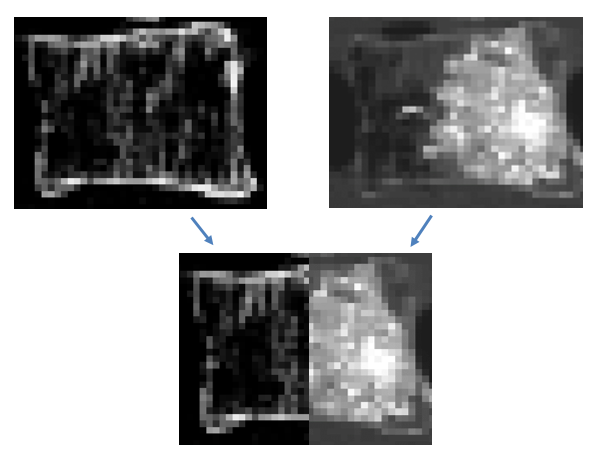
\includegraphics[width=4in]{Chapters/Chapter_HT_images/reg_demo.png}
  \caption{An illustration of the registration process, registering the non-augmented scan (left) with the augmented scan (right). The images are at 1 mm resolution, showing the artifacts created by the barium sulphate when viewed at this resolution, while to increase accuracy the registration carried out in Slicer 3D was at the full 82 $\mu$m resolution.}
  \label{fig:reg_demo}
\end{figure}

\subsubsection{Registered Scan Model Generation}

The augmented models using the registered scans were created in ScanIP, following similar methods to the bone volume fraction method described in Section~\ref{bvtv_method}.
The initial step was to import the registered augmented scans and apply an initial downsample to a resolution of 0.5 mm$^3$.
This resolution provided enough detail to capture the detail of the injected cement volume without increasing the computational difficulty and therefore time to segment the scans.

To segment the three regions (background, bone and endcaps, and injected cement) it was found that the most reproducible and accurate method was to use the Otsu thresholding process \cite{sezgin2004survey}, a filter that is built in to ScanIP\@.
It was used to find three masks in the scan and works on a threshold clustering method.
In this case searching for four clusters or masks separated by different thresholds and returning a mask that described the background, the bone and endcaps and the cement region.
From this only the cement mask was retained and underwent a flood fill filter, removing empty voxels found within the description of the mask.
The mask and background were then downsampled to 1 mm resolution and cropped to the same dimensions as the non-augmented model.
From the non-augmented model, the masked describing the vertebra, the endcaps and the background of the vertebra where imported.
The origin of the masks coming from the two backgrounds can be seen in \cref{fig:mask_demo}.

\begin{figure}[ht!]
  \centering
  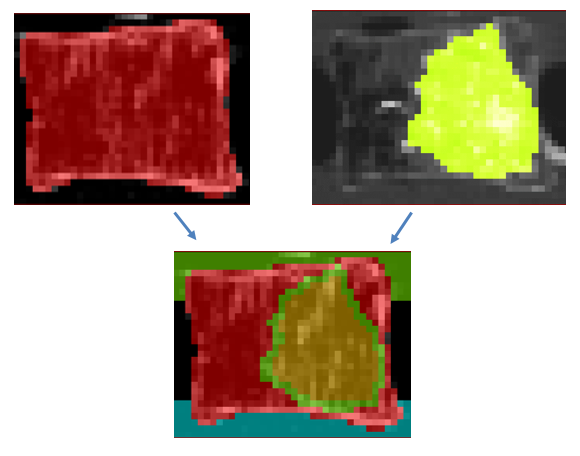
\includegraphics[width=4in]{Chapters/Chapter_HT_images/mask_demo.png}
  \caption{An illustration showing the origin of the masks from the non-augmented scan (left) and the augmented scan (right).}
  \label{fig:mask_demo}
\end{figure}


\subsubsection{Cement Volume Material Property Tests}

Based on the results of the tests carried out on the bovine tail vertebrae in \cref{chap_bov}, different material properties and approaches were attempted to further the agreement between the experimental and computational results of augmented vertebrae.
These were mainly changing the material properties of the interface layer between the bone and the cement, along with the material properties of the cement volume itself.

A different approach to modelling the cement region was also attempted.
This used an inverse greyscale material property for the cement region, rather than a homogeneous material property for the region, based on the greyscale background of the non-augmented vertebral scans with the mask from the augmented models overlaid.
This meant that darker regions of greyscale (within the cement volume) would be given a Young's modulus of PMMA cement (2.4 GPa) which would decrease linearly to the Young's modulus of the bone when entering into the brighter regions of the greyscale background.
Representing the cement regions using this method meant that the underlying bone present inside the cement volumes is not ignored, instead the interdigitation between bone and cement in represented.
While this representation is potentially inaccurate, it provides more detail that using a homogeneous material property and more detail than van be seen on the augmented vertebral scans.

The relationship for the cement volume using this method was therefore:
\begin{equation}
	E(\rho) = \alpha \rho + c
\end{equation}
\begin{equation}
	E(\rho) = -0.00842 \rho + 2.4
\end{equation}

Where $\rho$ is the greyscale value of each voxel and $E$ is the Young's modulus of each element within the cement region.
This ensured that the Young's modulus of the regions containing no bone (greyscale = 0)  was equal to that of the cement and regions containing bone (greyscale = 255) had a Young's modulus equal to 250 MPa, an approximate value for trabecular bone, with a linear relationship between.

Following the results of the above tests, the final material properties and boundary conditions for the augmented models are below.

The material properties for the yielding interface are:
\begin{itemize}
	\item 1 mm thick layer surrounding the cement volume (ScanIP dilate)
	\item Young's modulus =  0.01 MPa
	\item Poisson's ration = 0.4
	\item Yield stress = 5 Pa, upon which it becomes perfectly plastic
\end{itemize}

The material properties for the cement volume are:
\begin{itemize}
	\item Young's modulus =  1.7 GPa
	\item Poisson's ration = 0.4
\end{itemize}

Boundary conditions for the cement region include: tie contacts between the vertebrae and interface, and between the interface and the cement volume.
The remaining material properties and boundary conditions remain the same as with the non-augmented models.

\subsection{Measuring the Vertebral Body \& Augmentation Volume}

While the volume of the vertebral mask can be measured directly within ScanIP or Abaqus, this volume includes the remainder of the pedicles.
The size of the pedicles that remain after their removal during dissection varies between level and spine and is especially different with the level five vertebra, where the shape and size varies dramatically.
To account for this variation and to get a more accurate cement fill percentage for the augmented models elliptic cylinders were fitted to the vertebral body as shown in \cref{fig:cyl_fit}.



\begin{figure}[ht!]
  \centering
  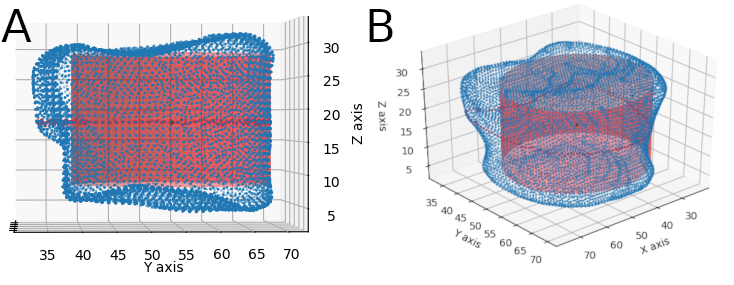
\includegraphics[width=5in]{Chapters/Chapter_HT_images/cyl_fit_ful_iso_both.png}
  \caption{A diagram showing the fitting of the cylinders to the vertebral body, where the point cloud describing the vertebra comes from an STL file, the red ring shows the points included in the mid-slice and the central red dot indicates the center of the mid-slice.}
  \label{fig:cyl_fit}
\end{figure}

Vertebrae that contained a vascular channel, seen in \cref{fig:cyl_channel}, had the channel removed by filling the space in ScanIP.
This was carried out for two main reasons: the first was to allow accurate fitting of the cylinder into the vertebral (to avoid the problems shown in \cref{fig:cyl_channel}) and to remove problems with the cement being exposed when modelling augmentation and the extra contacts / interfaces that are created.
Models with the vascular channel removed were compared to the original models and it was found that there was less than 0.5 \% difference for the set.
This was due to the elements used to fill the channel having material properties based on the greyscale, which had values of approximately zero, given the nature of the channel.
Due to the lack of any effect in removing the channel the vertebra models of augmentation did not include the vascular channel.

\begin{figure}[ht!]
  \centering
  \includegraphics[width=5in]{Chapters/Chapter_HT_images/cyl_fit_channel_both.png}
  \caption{An illustration showing the problems that occur with vertebrae that have a distinctive vascular channel and the false cylinder fit that occurs.}
  \label{fig:cyl_channel}
\end{figure}

This was carried out using a set of scripts written in python and rely of having stl files describing the vertebral geometry.
The scripts work by finding the middle slice of a set of nodes that describe the vertebra.
From the middle slice the shape of the ellipse is formed.
Given that the alignment of the vertebrae is uniform, the mid point on the $y$ axis is found by searching for the node furthest away from the weighted center, $\pm$ 2 mm of the weighted centre.
This gives the $a$ measure of the ellipse description.
The $b$ measure is found by using a similar process - searching for the node furthest away from the centre on the $x$ axis, within $\pm$ 2 mm.
The $a$ and $b$ measures gave the shape of the ellipse and the height of the elliptic cylinder was found by raising and lowering the ellipse until a node in the middle $\pm$ 5 mm intersected the ellipse.
This defined the height of the ellipse.
The volume of the ellipse was found (V = $\pi a b h$, where $a$ and $b$ have been described and $h$ is the height) and compared to that of the total vertebral volume, shown in \cref{tab:vertebrae_vol_cyl}.
The percentage reduction in vertebral body volume, from total vertebral body volume to the fitted cylinder volume, varies significantly and is due to changes to the vertebral shape outside of the main vertebral body portion.
For example, Spine 2 L1 was a degenerate vertebrae with extra bone growth at the anterior limits of the vertebral body.
Other large changes were due to the size of the pedicles, where larger vertebrae (Spine 4) had proportionally larger pedicles.

\begin{table}[ht!]
\centering
  \caption{Vertebral body volume compared to the volume of the fitted cylinder.}
	\label{tab:vertebrae_vol_cyl}
  \begin{tabular}{c |c|c|c}
	  Specimen & Total Vertebral  & Fitted Cylinder & Change in Volume\\ 
	  &Body Volume (mm$^3$)&Volume (mm$^3$) &(\%)\\ \hline \hline
	  Spine 1\_L1  & 31229 & 17490 & -44\\
	  Spine 1\_L2  & 31789 & 20551 & -35\\
	  Spine 1\_L3  & 33519 & 22014 & -34\\
	  Spine 1\_L4  & 35123 & 22796 & -35\\
	  Spine 1\_L5  & 31189 & 22254 & -28\\
	  Spine 2\_L1  & 33835 & 17420 & -48\\
	  Spine 3\_L1  & 45866 & 31073 & -32\\
	  Spine 3\_L2  & 53695 & 34470 & -36\\
	  Spine 3\_L3  & 56003 & 36750 & -34\\
	  Spine 4\_L1  & 35137 & 22231 & -37\\
	  Spine 4\_L2  & 36791 & 23837 & -35\\
	  Spine 4\_L3  & 39909 & 26036 & -35\\
	  Spine 4\_L4  & 43357 & 25612 & -41\\
	  Spine 4\_L5  & 45606 & 26936 & -41\\
	  \hline
  \end{tabular}

\end{table}

The effect of this change on the relationship between cement fill and change in augmentation stiffness was identified and is shown in \cref{fig:cyl_fit_comparison}.
While there was a change in the relationship, a clear trend between the cement fill percentage and change in stiffness for the majority of the vertebrae is still not evident without including other factors (described in \cref{sec:aug_stiffness_res}).

\begin{figure}[ht!]
  \centering
  \includegraphics[width=.7\textwidth]{Chapters/Chapter_HT_images/cyl_fit_comparison.png}
  \caption{The effect of using the fitted cylinder as a measure of vertebral body volume, on the relationship between augmentation fill volume and change in stiffness following augmentation. The red points show the relationship using the total vertebral volume, with the relationship using the fitted cylinder shown in blue.}
  \label{fig:cyl_fit_comparison}
\end{figure}





%TODO Other Methods - imageJ for images and 3d projections






\section{Results}


\subsection{Experimental Properties}\label{sec:aug_stiffness_res}

Material properties for the vertebrae can be seen in \cref{tab:bv_tv_anis}, with grouping evident for the bone volume fraction measurements.
For example the mean BV/TV value for Spine 1 was $0.159 \pm 0.026$, while the mean for Spine 4 was $0.248 \pm 0.022$ with similar results for the other two spines (although with less vertebra).
Less grouping could be seen between the degree of anisotropy for the vertebrae.

The vertebral stiffness following experimental loading can be seen in \cref{tab:aug_non_aug_stiff} for the non-augmented vertebrae and following vertebral augmentation.
The change in stiffness can be seen in \cref{fig:aug_non_aug_stiffness} where an increase in stiffness was seen Spine 1 L2-L5 and Spine 2 L1, while the remaining vertebrae presented a reduction in stiffness following augmentation.


\begin{table}[ht!]
	\caption{BV/TV and degree of anisotropy (DA) values found using the ImageJ
    plugin BoneJ tools Volume Fraction and Annisotropy respectively using a
    threshold of 18.}
	\label{tab:bv_tv_anis}
	\centering
	\begin{tabular}{c|c|c}
    Specimen                       & BV/TV & DA\\ \hline \hline
    Spine 1 L1  & 0.174 & 0.387 \\
    Spine 1 L2  & 0.17  & 0.364\\
    Spine 1 L3  & 0.137 & 0.359\\
    Spine 1 L4  & 0.127 & 0.418\\
    Spine 1 L5  & 0.187 & 0.341\\
    Spine 2 L1  & 0.391 & 0.199\\
    Spine 3 L1  & 0.255 & 0.327\\
    Spine 3 L2  & 0.267 & 0.231\\
    Spine 3 L3  & 0.281 & 0.301\\
    Spine 4 L1  & 0.257 & 0.239\\
    Spine 4 L2  & 0.241 & 0.338\\
    Spine 4 L3  & 0.244 & 0.348\\
    Spine 4 L4  & 0.247 & 0.371\\
    Spine 4 L5  & 0.249 & 0.186\\
    \hline
	\end{tabular}
\end{table}

\begin{table}[h!]
\centering
\caption{The experimental stiffness results for pre and post augmentation.}
\label{tab:aug_non_aug_stiff}
\begin{tabular}{c|c|c|c}
    Specimen  & Non-augmented Stiffness & Augmented Stiffness & Change in stiffness \\
              & (N/mm) & (N/mm) & (N/mm) \\ \hline \hline 
Spine 1 L1 & 2991          & 2339      & -652  \\
Spine 1 L2 & 3456          & 3980      & 523   \\
Spine 1 L3 & 3244          & 4152      & 907   \\
Spine 1 L4 & 3223          & 4744      & 1521  \\
Spine 1 L5 & 2891          & 4273      & 1382  \\
Spine 2 L1 & 6149          & 7119      & 969   \\
Spine 3 L1 & 5153          & 4444      & -709  \\
Spine 3 L2 & 5357          & 4848      & -510  \\
Spine 3 L3 & 5338          & 4779      & -559  \\
Spine 4 L1 & 3277          & 3231      & -46   \\
Spine 4 L2 & 5064          & 5042      & -22   \\
Spine 4 L3 & 6098          & 5749      & -349  \\
Spine 4 L4 & 4957          & 4488      & -468  \\
Spine 4 L5 & 7185          & 4403      & -2782 \\ \hline
\end{tabular}
\end{table}


\begin{figure}[h!]
  \centering
  \includegraphics[width=.7\textwidth,angle=270]{Chapters/Chapter_HT_images/aug_non_aug_stiffness}
	\caption{The experimental stiffness of the vertebrae pre and post augmentation. Showing that 5 of the 14 vertebrae showed an increase in stiffness following augmentation.}
  \label{fig:aug_non_aug_stiffness}
\end{figure}

A strong relationship was found between the percentage fill achieved and the bone volume fraction of the vertebra, where a reduced density of bone resulted in larger quantities of cement being injected into the vertebra before cement leakage occurred.
This relationship can be seen in \cref{fig:cmt_fill_vs_bvtv}.

\begin{figure}[ht!]
  \centering
  \includegraphics[width=.7\textwidth]{Chapters/Chapter_HT_images/cmt_fill_vs_bvtv.png}
	\caption{The relationship between the percentage cement fill of the total vertebral volume  achieved through the augmentation procedure and the bone volume fraction value for each vertebra. }
  \label{fig:cmt_fill_vs_bvtv}
\end{figure}

There was not a clear relationship found between the cement fill of the total vertebral volume and the resulting change in stiffness following augmentation for the set of vertebrae on the whole.
However, trends could be seen when splitting vertebrae into groups with: \textit{a)} dispersed volumes of injected cement and \textit{b)} concentrated volumes of cement.
This can be seen in \cref{fig:aug_cmt_fill_vs_ch_stiff} where a trend ($r=0.83$) can be seen between the percentage fill of the total vertebral volume and the percentage change in stiffness for those vertebrae with concentrated volumes of cement.

\begin{figure}[h!]
  \centering
  \includegraphics[width=.7\textwidth]{Chapters/Chapter_HT_images/Aug_cmt_fill_vs_ch_stiff.png}
	\caption{The relationship between the percentage fill of the total vertebral volume and the percentage change in the vertebral stiffness following augmentation. The line and \textit{r} value are for the red points where the cement volume was characterised as concentrated. The remaining blue points indicated the vertebra where the cement volume was characterised as dispersed.}
  \label{fig:aug_cmt_fill_vs_ch_stiff}
\end{figure}

\subsection{Experimental Augmentation}

The cement distributions following augmentation can be seen in \cref{fig:Spine 1_projection,fig:Spine 2_projection,fig:Spine 3_projection,fig:Spine 4_projection}.
From the 3D projection images and slices from $\mu$CT stack it was determined which vertebrae contained dispersed and which vertebrae contained concentrated volumes of cement, this characterisation can be seen in \cref{tab:conc_disp}.



\begin{figure}[ph!]
  \centering
  \includegraphics[width=.65\textwidth]{Chapters/Chapter_HT_images/G17-11_projections}
	\caption{Transverse and sagittal 3D projection views of the Spine 1 spine following augmentation, with the cement region being the brighter material in the vertebral body. The L1 vertebra is defined as having a dispersed volume of cement while the remaining L2, L3, L4, L5 vertebrae have concentrated volumes of cement.}
  \label{fig:Spine 1_projection}
\end{figure}

\begin{figure}[h!]
  \centering
  \includegraphics[width=.65\textwidth]{Chapters/Chapter_HT_images/G19-11_projections}
	\caption{Transverse and sagittal 3D projection views of the Spine 2 spine following augmentation, with the cement region being the brighter material in the vertebral body. The vertebra is defined as having a dispersed volume of cement.}
  \label{fig:Spine 2_projection}
\end{figure}

\begin{figure}[h!]
  \centering
  \includegraphics[width=.65\textwidth]{Chapters/Chapter_HT_images/G21-11_projections}
	\caption{Transverse and sagittal 3D projection views of the Spine 3 spine following augmentation, with the cement region being the brighter material in the vertebral body. The L1 vertebra is defined as having a dispersed volume of cement while the remaining L2 and L3 vertebrae have concentrated volumes of cement.}
  \label{fig:Spine 3_projection}
\end{figure}

\begin{figure}[ph!]
  \centering
  \includegraphics[width=.65\textwidth]{Chapters/Chapter_HT_images/G41-11_projections}
	\caption{Transverse and sagittal 3D projection views of the Spine 4 spine following augmentation, with the cement region being the brighter material in the vertebral body. The L1, L2 and L5 vertebrae are defined as having a dispersed volume of cement while the remaining L3 and L4 vertebrae have concentrated volumes of cement.}
  \label{fig:Spine 4_projection}
\end{figure}


\begin{table}[h!]
	\caption{The characterisation of the augmented vertebrae into vertebrae with dispersed and concentrated volumes of cement.}
	\label{tab:conc_disp}
	\centering
	\begin{tabular}{c|c}
    Vertebra & Cement Distribution \\
    \hline
    \hline

    Spine 1\_L1 & Dispersed \\
    Spine 1\_L2 & Concentrated\\
    Spine 1\_L3 & Concentrated\\
    Spine 1\_L4 & Concentrated\\
    Spine 1\_L5 & Concentrated\\
    Spine 2\_L1 & Dispersed \\
    Spine 3\_L1 & Dispersed \\
    Spine 3\_L2 & Concentrated\\
    Spine 3\_L3 & Concentrated\\
    Spine 4\_L1 & Dispersed \\
    Spine 4\_L2 & Dispersed \\
    Spine 4\_L3 & Concentrated\\
    Spine 4\_L4 & Concentrated\\
    Spine 4\_L5 & Dispersed \\
    \hline
	\end{tabular}
\end{table}



\subsection{Computational Results}


\subsubsection{Non-augmented Model Results}

The results of modelling the non-augmented vertebrae can be seen in \cref{fig:intact_norm_bvtv}, comparing the initial normal method (the method used with the bovine tail vertebra in the previous chapter) with the best case using the bone volume fraction method and the results of the sensitivity test described previously.
The results show a large improvement using the results of the sensitivity tests and the bone volume fraction method, with a concordance correlation coefficient improving from 0.55 to 0.86.

The effect of using the bone volume fraction method on the greyscale background
and colour map of the bone density can be seen in \cref{fig:compX4}, where the
much more clearly defined cortical shell and trabecular structure is evident.

\begin{figure}[h!]
  \centering
  \includegraphics[width=.65\textwidth, angle=270]{Chapters/Chapter_HT_images/intact_norm_bvtv}
	\caption{The results of using the normal method and the bone volume
	fraction method to model non-augmented human lumbar vertebrae. Red
shows the agreement using the normal method and blue shows the agreement using
the bone volume fraction method, with the orange dotted line showing perfect
agreement.}
	\label{fig:intact_norm_bvtv}
\end{figure}


\begin{figure}[h!]
  \centering
\includegraphics[width=.65\textwidth]{Chapters/Chapter_HT_images/compX4MethodAvsB.png}
\caption{A and B: The resultant 1 mm$^3$ greyscale background from the normal
and bone volume fraction method respectively, where the brightness in A has
been increased for visibility. C and D: a heat map of the greyscale values
through the mid slice of models from the normal and bone volume fraction method
respectively.}
	\label{fig:compX4}
\end{figure}

\subsubsection{Augmented Model Results}

The optimum results using the image registration and outcomes of the sensitivity tests can be seen in \cref{fig:aug_init_vs_best} with the blue triangles.
This registration method achieved a CCC = 0.46, while the initial method used (similar to the method used with the bovine tail vertebrae) achieved a CCC of 0.18.

\begin{figure}[h!]
  \centering
	\includegraphics[width=.65\textwidth, angle=270]{Chapters/Chapter_HT_images/aug_init_vs_best}
	\caption{The results of using the initial method (red circles) and the registration method (blue triangles), showing the agreement to the perfect x=y line in orange.}
	\label{fig:aug_init_vs_best}
\end{figure}
















\section{Discussion}





\subsection{Experimental Results}

Experimentally there was large variation seen in the results, in terms of
material properties (BV/TV values), geometry and response to loading.  The
experimental response to loading showed a large range in the stiffness of the
vertebrae, even for vertebrae with similar volumes and for vertebrae
originating from the same spine.  This wide range of stiffness' extends to the
augmented vertebral stiffness, although the range does decrease following
augmentation.  The variation seen in the intact vertebrae aids the
justification for the study, if such a wide range of vertebral properties
exists within such a small data set then it explains why such variation is
found clinically when identifying the response to vertebroplasty.

Following augmentation five of the 14 vertebrae showed an increase in the
stiffness following augmentation, which, given the stiffness of the injected
cement compared to that of trabecular bone, is an unexpectedly small number.
Four of the vertebrae that showed an increase in stiffness were from the same
spine (Spine 1), which is the spine that had a considerably smaller bone volume
fraction compared to the other vertebra from other spines.  Given that this
spine had the smallest bone volume fraction it also received the largest
quantity of cement, given the relationship between the percentage fill achieved
and the bone volume fraction.  This relationship is most likely due to the ease
of cement injection before leakage, with more dense vertebrae failing to
receive large volumes of cement before the cement found one of the vascular
channels (upon which injection was stopped) and less dense vertebrae having
more space to receive cement.

Cement volume positions were generally to the anterior of the vertebrae and to
the middle of the inferior-superior plane, matching the desired position
achieved through the insertion of the needle and angling of the side opening
needle tip.  Given the lack of obvious variation in cement positions and shapes
it was difficult to characterise the cement distributions, hence, a simplified
description of the cement was used.  This simplified description of the cement
described whether the cement was in a concentrated volume or dispersed in a
larger region or whole vertebra.  Following this characterisation strong
relationships were found between the change in stiffness and percentage fill,
if only those vertebrae with a concentrated volume of cement were included.
Suggesting that distributed volumes of cement are difficult to predict and
should be avoided when carrying out the procedure using fluoroscopy, especially
with more dense vertebrae where the likelihood or disperse volumes of cement
increased.


To summarise the change in stiffness following augmentation based on the
material properties of the vertebrae, the following features have the greatest
effect:
\begin{enumerate} 
\item A smaller bone volume fraction results in larger quantities of cement
    being injected before leakage occurs.  
\item If the volume of cement is contained in a concentrated volume then the
    greater the volume of cement then the larger the increase in stiffness
    following augmentation.  
\item If the volume of cement is dispersed through the
    vertebral body then there is no relationship between the volume of cement
    injected and its effect of the vertebral stiffness.
\item Concentrated volumes of cement are more likely if the bone volume
fraction of the vertebra is smaller.
\end{enumerate}

The effects of vertebral geometry and material properties on the response to
augmentation will be investigated further using statistical shape modelling in
\cref{PCA_CHAP}, giving a more detailed story of the suggested approaches to
vertebroplasty based on the tests carried out in this study.

\subsection{Limitations Regarding Specimen Numbers \& Vertebral Features}

One of the main limitations to the study is the numbers of vertebrae included
in in the set.  Having four human spines with a limited number of lumbar
vertebrae available from each spine, meant that only 14 out of a possible 20
vertebrae were able to be tested.  This meant that there was a skew towards the
top of the lumbar section with limited numbers of L4 and L5 vertebrae.  Such
skews to the data set have effects to any statistics applied to the data set
and will be discussed more thoroughly in the PCA discussion chapter in
Section~\ref{pca_disc}.  More relevant to modelling the vertebrae is the effect
this has on the determination and optimisation of the greyscale conversion
factor.  The large change in geometry from L4 to L5, rather that the gradual
change between L1 to L4, introduces questions about the response to loading
(and augmentation) for this vertebra in particular and how it differs from
other levels.  A resolution to this limitation would be to increase the
specimen numbers and look at vertebral levels in isolation; identifying level
specific differences and properties.  Variation at different vertebral levels
may require level specific greyscale conversion factors, such as those required
when modelling different animal species \cite{zapata2017methodology}.  However,
within the current set of vertebrae greater variation was found between spine
rather than level (for BV/TV, stiffness and vertebral body volume), even when
including L5 vertebrae.  Suggesting that segregation of vertebral levels is
unnecessary for the current specimen set. 

Another limitation of the study is the age range and limited information
regarding vertebral health.  Because of this unknown vertebral quality or
health it was decided to skip the initial load to failure carried out in the
bovine tail study.  While no evidence of fractures could be seen in the $\mu$CT
scans, other than slight wedge shapes, there was no evidence of the bovine tail
vertebrae having succumbed to fracture in $\mu$CT either, despite clear
fractures on load displacement curves.  Therefore the state of the vertebrae
was relatively unknown pre-augmentation and the study therefore becomes an
investigation into the effects of prophylactic vertebroplasty, although with
the possibility that some of the vertebrae were fractured \textit{in vivo}.




\subsection{Computational Results}

The improvement in the agreement between computational stiffness and the
experimental stiffness results using the bone volume fraction method and the
results of the sensitivity tests is significant and provided a good foundation
for modelling the more challenging augmented models.  The improvement using the
bone volume fraction method in isolation (without the results of the other
sensitivity tests) showed a large improvement over the normal method.  The
normal method performed similarly on the bovine tail vertebrae as with the
human lumbar vertebrae, with a CCC = 0.49 for bovine tail vertebrae and CCC =
0.55 for the human vertebrae. 

The improved agreement of modelling the human vertebrae over the bovine
vertebrae when using the same ``normal" method suggests that either the human
vertebrae are more receptive to the modelling method used, or that the
experimental procedure was more repeatable and therefore provided more accurate
results. One possibility is that the less narrow human vertebrae provided an
easier material to load axially, with slight off axis loads causing the
vertebrae to not be seated in the endcaps correctly in the case of the bovine
tail vertebrae. This sensitivity to endcap contact properties was shown earlier
and potentially given the tendency of the bovine vertebrae to be loaded
non-axially they may be more sensitive to such endcap contact properties. So,
while experimentally the bovine vertebrae were able to slip in the endcaps,
computationally the two materials were tied, restricting this ability and
reducing the agreement with the experiment. Conversely, the wider human
vertebrae had less of a tendency to slip and were less sensitive to the endcap
contact.

The improvement using the bone volume fraction method is most likely due to the
added definition of the trabecular bone and cortical shell, especially given
how important the correct representation of load sharing is for accurate models
\cite{eswaran2006cortical}. This agreement is much stronger than the agreement
found in similar studies that used a comparable methodology to the ``normal"
method \cite{Wijayathunga2008, zapata2017methodology, RobsonBrown2014} and
comparable to methods that used more complex though individual material
properties for each model \cite{Kinzl2012,kinzl2013experimentally}.  Having
greater definition of the cortical shell and trabecular bone alignment allows
much more accurate descriptions of the load transfer through the vertebrae,
rather than the more simple description with the more homogenised material
properties of the normal method.

This method also removed any effect that the bone marrow, where, given the
freeze/thaw cycles the marrow leaks from the vertebrae giving vertebral scans
with portions of the bone marrow missing and therefore changing the greyscale
background and material properties.  Due to the initial segmentation at 82
$\mu$m using the BV/TV method the bone marrow is not present in the segmented
full resolution or downsampled scans and therefore has no impact on the
material properties of the models.  Conversely, using the normal method, areas
lacking bone marrow would have a lower Young's modulus and areas with bone
marrow would have higher Young's moduli, not corresponding to the actual
properties of these regions and changing the load distribution.

One of the limitations of the bone volume fraction method is that is relies on
having trabecular resolution scans of the vertebrae to apply the trabecular
bone thresholds to.  This limits the origin of the scans to \textit{in vitro}
scans rather than \textit{in vivo} scans where the resolution is limited to
approximately 1 mm and larger.  Given the intention to generate larger
populations of vertebra models for use in statistical shape modelling this
limit to scan origin is an unwanted consequence.  A possible solution to this
problem would be to use 16 bit images rather than the currently used 8 bit
images.  This change gives an increase in the number of greyscale values
available from the 256 of 8-bit images to over 65,000 for 16-bit images.  The
main benefit of the bone volume fraction method is the increased definition of
bone structure and a greater contrast between the brighter, denser cortical
bone, the trabecular bone and the empty, non-bone areas.  Using 16-bit images
along with image manipulation to change the contrast of the scans may allow the
added detail and contrast to be captured with relatively low ($\geq$ 1 mm)
resolution scans, therefore greatly increasing the number of vertebral
specimens available for use. An example of how this could be achieved is shown
in \cref{fig:adding_contrast} where the background from the normal method has
been edited through adjusting the contrast to give a similar background to that
achieved using the bone volume fraction method. The detail in the centre of the
vertebral body is less clear in this example, however, it was achieved through
simple contrast manipulation meaning that more trabecular detail could be
preserved using a curves (remapping of the image tonality) or as already
proposed 16 bit images.

\begin{figure}[h!]
  \centering
\includegraphics[width=.65\textwidth]{Chapters/Chapter_HT_images/adding_contrast.png}
\caption{An example showing the ability to create a greyscale background similar to that achieved using the BV/TV method, but instead adjusting the contrast of the background from the normal method.}
	\label{fig:adding_contrast}
\end{figure}


The results of modelling augmented vertebrae showed a reduction in the
agreement when compared to the non-augmented vertebral models.  Reasons for
this are centred around modelling the internal cement volume, given the good
agreement seen between the non-augmented vertebrae and their models.  More
specifically the problems in modelling the cement region within models may be
due to experimental and modelling techniques.  Issues surrounding the
experimental work are the difficulty in capturing the extent of the
augmentation volume, often due to clumping of the barium sulphate and
separation of the barium sulphate from the other components of the PMMA cement.
While this problem is minimised through segmentation of the cement region at
higher resolutions before the downsampling, a problem still lies in capturing
the intricate interdigitation between the cement and the trabecular bone at a
resolution of 1 mm.  An additional experimental challenge is the unknown level
of damage caused to the vertebrae when the needle is inserted.  Given that
after clear fractures (based on load-displacement curves) could not be seen on
82 $\mu$m scans of bovine tail vertebrae, it is unlikely that micro-fractures
caused through needle insertion will be captured in the $\mu$CT scans of the
human vertebrae.

Despite the reduced agreement of the augmented models, there was a large
improvement compared to the initial method, which was the method used for
modelling augmentation in the bovine tail vertebrae.  As with the non-augmented
models the CCC using the initial method was very similar to the CCC using the
similar method on the bovine tail vertebrae, CCC = 0.18 and 0.15 for the human
and bovine models respectively.  This makes the improvement using the
registration significant and a beneficial step in making the models.

Achieving improved agreement between the computation and experimental models is
an obvious next step for the project and despite the range of approaches used
and attempted to improve the agreement, there are some next steps.  Given the
difficulty capturing the detail between the cement and trabecular bone, using a
higher resolution is a clear next step.  However, it comes with a number of
difficulties which have been shown in the study by Zhao et al. \cite{Zhao2012},
where the increase in resolution presents many other unknowns that need to be
modelled.  For example modelling the specific interaction between the bone and
the cement including the  coefficient of friction between them.  This would
require difficult experimental investigations, given the unique environment
inside the vertebrae filled with bone marrow.  Along with modelling properties
that are not applicable in continuum level models, there is the problem with
computational cost, where the increased time to solve models would become
problematic given the investigatory nature of the study and the fact that the
behaviour in simplified bone plug models is different to what is seen in whole
vertebrae \cite{Sikora2013}.

\subsubsection{Sensitivity Test Significance and Influence on Errors}

Sources of error from the modelling side come from discrepancies between the
experimental setup and specimen geometry. Sensitivity tests carried out
identified the effect of errors in accurately describing the cement cap depth
and loading position accuracy, given the 1~mm accuracy limit. The maximum
possible error for load position in a $\pm$1~mm anterior/posterior direction
was less than 5\%, with the worst case error for the for the encap depth tests
(1~mm thicker for both endcaps) being approximately 5\%. Other possible errors
would include accurately capturing the model geometry, however simply eroding
or dilating the vertebral mesh would not accurately describe the type of
meshing errors that may occur (it is unlikely that masks would be created at
$\pm$ 1 voxel around the whole model). To attempt to answer this a user
variability test was carried out in \cref{sec:uvs}. There, the maximum user
variability gave errors of 14 \%, however as discussed in that chapter, users
achieved consistently higher or lower stiffness' compared to their peers.
Hence, a 14 \% error within a single users segmentation process is both
unlikely and further reduced through the use of the python script carrying out
the thresholding and morphological filters to segment the model.

Changing the endcap depth presents an interesting study into the effects of
over constraining the models. For the models with the tied constraints changing
the endcap depth had a different effect for the two vertebrae (although the
same overall trend, where thicker endcaps led to more constraint and therefore
higher stiffness values). The spine 1 L2 vertebrae was equally sensitive to
changing the superior and inferior depth, although gave a smaller effect when
the depth was reduced (exposing more bone). The spine 4 L5 vertebrae was much
more sensitive to changing the inferior endcap, especially when reducing the
depth of the endcap. This large reduction in the stiffness when removing 3 mm
of endcap material from the inferior endcap of approximately 20 \% is caused by
exposing a less dense area of bone, which, when no longer supported by the tied
endcap resulted in the reduced stiffness. Other than this specific effect the
general trend was an increased sensitivity to increasing the cement depth, with
a much smaller sensitivity to exposing more bone.

Changing the endcap depths when the frictionless contact was used resulted in
(for the most part) much less sensitivity to changing the endcap depth, when
compared to the tied endcap models. The exception is the spine 4 L5 vertebra,
where when the endcap depth is reduced a very large decrease in the stiffness
is seen.

\subsubsection{Computational Method Significance}

\section{Conclusion}








\chapter{Principal Component Analysis \& Statistical Shape \& Appearance Modelling}\label{PCA_CHAP}


\section{Introduction}

\subsection{Aims of Statistical Shape \& Appearance Models}

\subsection{General Methodology}

Generally SSAMs start with a rigid registration, where rotations and translations are applied to all meshes or models that form the input data set so that they share a common coordinate system.
Methods of performing the rigid registration often use an automated approach where certain degrees of freedom are restricted to ensure registration is achieved.



\section{Methods}

\subsection{Measuring Vertebral Geometry}

Vertebral volume or the vertebral body volume may be the easiest and most obvious measure of geometric change within a set of vertebra.
It has been shown in Chapter \ref{Chapter_HT} that there is a strong correlation between vertebral size and stiffness and so this may be enough for a range of comparisons between spines and individual vertebrae.
However, the input set of vertebrae contain a wide range of variation which can be seen visually, which may play an important role in the effect of cement augmentation and is another method of validating the outputs from the PCA generated set of models.

Measuring vertebral geometries in previous studies have either taken the measurements from x-ray scans \cite{Gilad1986,Gilad1985} or $\mu$CT scans \cite{Zhou2000,Cheung1994}, where the measurements have been made through the moving a cursor to the locations of specific points and reporting the distance between them.
While this method may produce accurate results, there is inherent human error associated, the number of measurements is limited to the number of planes available and applying this to large sets of data is time consuming which may lead to further error.

The approach used here involves using the 1 mm voxel resolution models generated in ScanIP (v. 2016) which are are used for FE modelling.
The mask describing the vertebral body of these vertebrae is exported as a stereolithography file (STL), allowing the surface of the vertebra to be measured.
Measuring the vertebra was carried out in Matlab where the STL file was imported forming a point cloud describing the surface from the surface nodes.
Once imported the point cloud was split into thirds in each of the three anatomical planes, with the points describing the vertebra within these thirds being stored in nine array variables.
Cuboids were then fitted to the 3D arrays, maintaining the correct alignment and therefore prohibiting rotation of the cuboid.
The cuboid fits can be seen in \cref{fig:cuboid_ax, fig:cuboid_sag, fig:cuboid_cor}.


\begin{figure}[ht!]
  \centering
  \includegraphics[width=4in]{Chapters/Chapter_PCA_images/Cuboid_fit_axial.png}
  \caption{The three cuboids fitted to the vertebra point cloud in the axial plane.}
  \label{fig:cuboid_ax}
\end{figure}

\begin{figure}[ht!]
  \centering
  \includegraphics[width=4in]{Chapters/Chapter_PCA_images/Cuboid_fit_coronal.png}
  \caption{The three cuboids fitted to the vertebra point cloud in the coronal plane.}
  \label{fig:cuboid_cor}
\end{figure}

\begin{figure}[ht!]
  \centering
  \includegraphics[width=4in]{Chapters/Chapter_PCA_images/Cuboid_fit_sagital.png}
  \caption{The three cuboids fitted to the vertebra point cloud in the sagital plane.}
  \label{fig:cuboid_sag}
\end{figure}

Measuring the two longer sides of the fitted cuboids gives a total of 18 measurements describing most aspects of the vertebral geometry, these can be seen with their abbreviations in Table \ref{tab:measurements}.
This includes identifying wedge shaped vertebrae, recorded as reduced anterior height compared to the posterior height, left to right wedge shapes, recorded as sagital left height being smaller or larger when compared to the sagital right height.

\begin{table}[ht!]
	\caption{The measurements and abbreviations taken from the vertebrae.}
	\label{tab:measurements}
	\centering
	\begin{tabular}{c|c}
    Measurement & Abbreviation \\
    \hline
    \hline
    Sagital Left Height & SLH \\
	Sagital Left Depth & SLD \\
    Sagital Mid Height & SMH \\
	Sagital Mid Depth & SMD \\
    Sagital Right Height & SRH \\
	Sagital Right Depth & SRD \\
	Coronal Anterior Height & CAH \\
	Coronal Anterior Width & CAW \\
	Coronal Mid Height & CMH \\
	Coronal Mid Width & CMW \\
	Coronal Posterior Height & CPH \\
	Coronal Posterior Width & CPW \\
	Axial Inferior Depth & AID \\
	Axial Inferior Width & AIW \\
	Axial Mid Depth & AMD \\
	Axial Mid Width & AMW \\
	Axial Superior Depth & ASD \\
	Axial Superior Width & ASW \\
	\hline
	\end{tabular}
\end{table}

The plugin for ScanIP that allows principal component analysis and the generation of models described by the principal components consists of five main steps.

The first of these steps is a pre-processing step, converting the masks and backgrounds into nessessary formats (.mha \& .mhd) for use with the ITK toolkit.

The following step carries out rigid registration of the models, aligning the masks and backgrounds to a shared coordinate system.
This is carried out using the ITK library with the registration being measured according to a mean squared image-to-image metric using a gradient descent optimiser.
A limit to the number of attempts or steps allowed can be set; the default value of 100 steps for each input model was used.

The geometry of each input specimen was described in a deformable registration step, measuring the transform required to morph the mean of the input vertebrae onto each of the input vertebrae.
This step utilises the ITK FEM registration filter.

Penultimately, the transforms between the mean and each of the input vertebrae which describe the vertebral geometries are used as inputs for PCA.
Here the outputs of the step include the principal components, their eigenvalue, percentage of variation captured in that component and the cumulative percentage variation captured.

Finally, the SSAM produced can be used with the ITK Image Warp filter to generate new mask and background combinations from within the envelope of geometric and material property variation created by the input set, according to the principal components.
The plugin allows for the first five principal components (PC1, PC2, PC3, PC4 \& PC5) to be used for as variables for model generation, altering the value of the principal components by up to three standard deviations away from the mean in both positive and negative directions.

\subsection{Generating Vertebrae Models}

\subsubsection{Range of Shapes Generated}

To attempt to understand what each of the principal components represented in terms of the variation captured by it, models were created at $\pm$1, $\pm$2 and $\pm$3 standard deviations away from the mean for the first three principal components independently.
In addition to these, the mean model was generated, allowing comparisons of the other generated models against it.

Finally, in order to know whether the range of geometries, material properties and resultant stiffnesses found in the input set was represented in the SSAM within the first three principal components, models were generated which incorporated the variation found in PC1, PC2 \& PC3.
These models would represent the corners of a cube who's axis would be PC1, 2 \& 3 and who's origin would be the mean vertebra.
If the majority of input models (68 \%, representing the quantity of the population expected to fit within $\pm$1 SD of the mean for a normally distributed input set) fit within the limits created by a cube with side length from +1 to -1 SD along each axis for geometric measurements, greyscale background and resultant stiffness, then the variation of the input set will have been captured and represented by the SSAM.

\subsubsection{FE Model Setup}

Once the vertebrae were generated using the plugin the rest of the FE model was set up.
This included forming endcaps to mimic the experimental setup and how the input set was loaded.
Endcaps were created programmaticaly within the ScanIP python scripting environment with a diameter of 90 mm, approximately equal to the diameter of the experimental endcaps, with a depth of 6 mm ensuring the superior and inferior tips of the vertebrae were captured with a minimum of 1 mm between the vertebra and end of the cement.
The remaining properties for the FE model are identical to those used for the models of the human vertebra which became the inputs to the PCA plugin.
This includes a tied interaction between the vertebrae and endcaps and material properties for the endcaps being: Young's modulus 2.45 GPa and Poissons's ratio of 0.3.
Material properties for the vertebra used the same greyscale approach as in previous chapters with the Young's modulus for each element being:
\[ E = GS \times \alpha \]
Where, $GS$ is the greyscale value for the current element (between 0 and 255) and $\alpha$ is the conversion factor.
The conversion factor used has the same value used previously for the non-augmented set of vertebrae: $\alpha = 0.0008184$.
Applying load to the models is carried out as in the previous chapter, with 1 mm of displacement applied to a loading point, with the reaction force being measured to obtain the stiffness.
The loading point is found by finding the centre of the vertebral body in the middle slice axially and translating the point axially to the maximum height of the model, including endcaps.
The load is then applied through a plate which is tied to the superior endcap.

\subsubsection{Augmentation in Generated Models}




\section{Results}

\subsection{Validating Generated Vertebrae} \label{sec:pca_val}

Validation of the generated vertebrae from the PCA plugin for scanIP is vital for ensuring any results are sensible, for example when artificially augmenting the vertebrae, and to ensure that the modes of variation previously described are genuine descriptions of the variation found within the input set.
To achieve this validation, aspects important to the generated models need to be compared to the variables found in the input set.
The variables compared will be the geometry and volume of the vertebrae, the greyscale background and therefore the material properties of the models and finally the resulting stiffness when loads are simulated on the generated FE model.
While identifying the modes of variation in isolation are important to characterise how such variation affects the outcomes of augmentation or understanding the content and main modes of variation, combinations of the principal components generate different models that may describe different ranges of variation.
Therefore, the variation found within one standard deviation of the mean for the first three principal components, including all of the combinations of standard deviations within $\pm$ 1 SD, including the mean.
For example, PC 1 +1, PC 2 +1, PC 3 -1, would be one model with a combination of the first three principal components.

\subsubsection{Geometry Validation}

Identifying the variation in geometry for combinations of the first three principal components, with all possible combinations within $\pm$1 SD of the mean is presented here.
The 18 geometric measures found within the $\pm$1 SD models are presented in \cref{fig:pca_cube}. 
The results presented here show a strong agreement between the input and the generated models, with the means of the two sets agreeing closely, along with the range of the measurements.
Outliers in the input set originate from the bone spurs and other features of the degenerated vertebrae. %TODO add image of G19 L1
Differences in the range of generated vertebrae compared to the range of measurements seen in the input set are due to the input set describing only one standard deviation of variation.

Volume differences between the input set and generated vertebrae were also small, with the difference between the mean of the input set volume and the mean generated model volume being 10 \%, the means being 39500 mm$^3$ and 38245 mm$^3$ respectively.
The range of vertebral volumes is also comparable: the input set range is 31189 to 56003 mm$^3$ while the generated vertebrae for $\pm$1 SD with all possible combinations of PC 1, 2 and 3, have a range of 28152 to 50462 mm$^3$.

\begin{figure}[h!]
  \centering
  \includegraphics[width=\textwidth]{Chapters/Chapter_PCA_images/pca_cube.pdf}
	\caption[Geometric variation in the generated vertebrae.]{The variation in the 18 geometric measures of the input set models compared to the variation in the generated models for the first three principal components including all combinations of the +1, mean and -1 standard deviations.}
  \label{fig:pca_cube}
\end{figure}

\subsubsection{Material Property (Greyscale) Validation}


The variation seen in the histograms representing the greyscale differences between generated models and the input can be seen in \cref{fig:pca1_histo,fig:pca2_histo,fig:pca3_histo}, with the range of histograms from the input set shown as the grey range and the coloured lines showing the histogram for each of the generated models.
This normalised data shows a general agreement with the shape of the curves and relative quantities being very similar.
Deviations from the similarity are, for the most part, at the high and low greyscale values, where in general there are less voxels in this range for the generated models.
Comparing these results to an example background in \cref{fig:input_gen_background}, comparing an input background slice with the mean generated model mid-slice, shows that the lack of voxel counts in the high and low greyscale regions correlates with having less contrast between the densest bone in the cortical shell and the empty parts.
Additionally, \cref{fig:input_gen_background} shows that the important feature for load transfer, the cortical shell, is preserved and accurately described in the background of the mean generated model.
While the cortical shell's presence is clear, it's definition and contrast between it and the trabecular bone or empty spaces is not as well preserved.
Other features such as the posterior vascular channel is also preserved, albeit not as clearly as the features on the input set.

Differences in the mean greyscale between the input set and the generated models of all combinations of $\pm$1 SD are 108 and 97 respectively.
The ranges are 78 to 164 for the input set and 72 to 122 for the generated models for all combinations of $\pm$1 SD.
\begin{figure}[h!]
  \centering
  \includegraphics[width=.65\textwidth]{Chapters/Chapter_PCA_images/pca1_histo.pdf}
  \caption{Histogram of the models generated from principal component 1, with $\pm$ 3, 2 \& 1 standard deviations away from the mean. The values are normalised with respect to the total volume of the vertebrae, allowing comparisons with different sized model. The grey background represents the range of histograms seen in the input set.}
  \label{fig:pca1_histo}
\end{figure}

\begin{figure}[h!]
  \centering
  \includegraphics[width=.65\textwidth]{Chapters/Chapter_PCA_images/pca2_histo.pdf}
  \caption{Histogram of the models generated from principal component 2, with $\pm$ 3, 2 \& 1 standard deviations away from the mean. The values are normalised with respect to the total volume of the vertebrae, allowing comparisons with different sized model. The grey background represents the range of histograms seen in the input set.}
  \label{fig:pca2_histo}
\end{figure}

\begin{figure}[h!]
  \centering
  \includegraphics[width=.65\textwidth]{Chapters/Chapter_PCA_images/pca3_histo.pdf}
  \caption{Histogram of the models generated from principal component 3, with $\pm$ 3, 2 \& 1 standard deviations away from the mean. The values are normalised with respect to the total volume of the vertebrae, allowing comparisons with different sized model. The grey background represents the range of histograms seen in the input set.}
  \label{fig:pca3_histo}
\end{figure}

\begin{figure}[h!]
  \centering
  \includegraphics[width=.6\textwidth]{Chapters/Chapter_PCA_images/INPUT_GEN_BACKGROUND.png}
	\caption{Greyscale backgrounds for the axial mid-slice from, A, the Spine 1 L1 input vertebra and B, the mean generated model.}
  \label{fig:input_gen_background}
\end{figure}
\subsubsection{Resulting Stiffness Validation}

\begin{table}[]
\centering
\caption{My caption}
\label{tab:stiffness_gen_models}
\begin{tabular}{c|c|c}
Model  & Stiffness (N/mm) & Fractional Change from the Mean \\ \hline \hline
PC1 +3 & 6543.38          & 1.582                           \\
PC1 +2 & 5887.75          & 1.424                           \\
PC1 +1 & 5059.89          & 1.224                           \\
Mean   & 4134.88          & 1.000                           \\
PC1 -1 & 2962.82          & 0.717                           \\
PC1 -2 & 1696.47          & 0.410                           \\
PC1 -3 & 1131.86          & 0.274                           \\ \hline
PC2 +3 & 4159.29          & 0.980                           \\
PC2 +2 & 4291.53          & 0.831                           \\
PC2 +1 & 4355.98          & 0.770                           \\
Mean   & 4134.88          & 1.000                           \\
PC2 -1 & 4051.57          & 1.006                           \\
PC2 -2 & 3434.91          & 1.038                           \\
PC2 -3 & 3182.81          & 1.053                           \\ \hline
PC3 +3 & 2930.69          & 0.709                           \\
PC3 +2 & 3420.55          & 0.827                           \\
PC3 +1 & 3846.57          & 0.930                           \\
Mean   & 4134.88          & 1.000                           \\
PC3 -1 & 4409.05          & 1.066                           \\
PC3 -2 & 4240.58          & 1.026                           \\ \hline
PC3 -3 & 4141.31          & 1.002                          
\end{tabular}
\end{table}


\subsection{Measuring \& Interrogating Vertebral Variation}

\subsubsection{Geometry Variation}

The geometric variation found in the first three principal components has been identified using the images of the surface point clouds of the mean and +3 and -3 standard deviations away from the mean, along with the measurements of the 18 variables described previously.
The images of the point clouds can be seen in \cref{fig:PC1_2_3_Axial,fig:PC1_2_3_Sagital,fig:PC1_2_3_Coronal}, showing the view of the vertebral models from the three anatomical planes with a three-dimensional view in \cref{fig:PC1_2_3_3D}.
More simplified figures can be seen in \cref{fig:PC1_2_3_AxialSlice,fig:PC1_2_3_SagitalSlice,fig:PC1_2_3_CoronalSlice}, showing the mid-slice through each of the anatomical planes, while information is lost here, it allows an clear visualisation of the modes of variation found in the main parts of the vertebral body.
Here, only the +3, mean and -3 standard deviations of the principal components are shown, this simplifies and allows clear visualisations of the main mode of variation present in each principal component.
A quantification of the change in volume can be seen in \cref{tab:pca_geo_tab} for the mean and $\pm$ 1, 2 \& 3 standard deviations away from the mean.

Principal component one contains the least geometric variation of the first three principal components.
The mid slice axially shows an almost identical shape and size between the +3, mean and -3 standard deviations, while the coronal and sagittal planes show minor changes in the overall size and volume of the vertebrae.
The changes in total vertebral volume is limited to 17 \% larger and 15 \% smaller than the mean model, shown in \cref{tab:pca_geo_tab}.

Principal component two shows the most interesting geometric variation with many of the different shapes and some of the degeneration of the input set clearly visible.
The large changes to the axial mid slice (\cref{fig:PC1_2_3_AxialSlice}) of the second principal component appear to represent the different levels of the lumbar spine that made up the input set.
Positive standard deviations away from the mean, especially the +3 SD slice has the much wider posterior portion aligning with that of the L5 lumbar vertebrae.
Conversely the much narrower -3 SD model appears similar to the L1 lumbar vertebrae.
This change in width between the +3 and -3 SD is especially evident in the coronal views in \cref{fig:PC1_2_3_CoronalSlice}.
This change from vertebra reminiscent of L5 vertebrae at +3 SD to L1 vertebra at -3 SD (and therefore L3 vertebrae in the mean model) is also reflected in the sagittal views (\cref{fig:PC1_2_3_SagitalSlice}) where anterior and posterior wedge shapes can be seen in the +3 and -3 SD models respectively.

Finally, principal component three also contains a considerable quantity of the geometric variation, although much more simple.
Here, the mode of geometric variation is the size of the vertebrae with the -3 SD model being considerably larger than the mean vertebral model (54 \% larger) and vice versa with the +3 SD model, where its volume is much smaller than the mean vertebra (40 \% smaller).

Quantification of all of the measurements taken on the generated models can be seen in \cref{tab:pca_geo_tab} with the acronyms for the measurements given in \cref{tab:measurements}.
The colouration in the table allows easy identification of the changes to the vertebral geometry compared to the mean generated model, for example, while the changes to the measurements are near uniform in PC 1 \& 3, the non-uniform nature of PC 2 shows the different shapes that are present and described above.
Additionally it allows quantification of the shapes seen in the models, for example the anterior and posterior wedge shapes in PC 2, described with the Coronal Anterior Height and the Coronal Posterior Height having an antagonistic relationship.
However, the main benefit of the table and its measurements is for the validation of the PC models against the input set, ensuring that the shapes measured in the input set are represented in the models.
This is described in \cref{sec:pca_val}.


\begin{figure}[p]
  \centering
  \includegraphics[width=.65\textwidth]{Chapters/Chapter_PCA_images/PC1_2_3_Axial.pdf}
  \caption{Axial views of the surface point clouds of the vertebral models from the first three principal components, showing the mean, +3 and -3 standard deviations away from the mean. Showing how the geometry is captured in the first three principal components.}
  \label{fig:PC1_2_3_Axial}
\end{figure}

\begin{figure}[p]
  \centering
  \includegraphics[width=.65\textwidth]{Chapters/Chapter_PCA_images/PC1_2_3_Sagital.pdf}
  \caption{Sagittal views of the surface point clouds of the vertebral models from the first three principal components, showing the mean, +3 and -3 standard deviations away from the mean. Showing how the geometry is captured in the first three principal components.}
  \label{fig:PC1_2_3_Sagital}
\end{figure}

\begin{figure}[p]
  \centering
  \includegraphics[width=.65\textwidth]{Chapters/Chapter_PCA_images/PC1_2_3_Coronal.pdf}
  \caption{Coronal views of the surface point clouds of the vertebral models from the first three principal components, showing the mean, +3 and -3 standard deviations away from the mean. Showing how the geometry is captured in the first three principal components.}
  \label{fig:PC1_2_3_Coronal}
\end{figure}



\begin{figure}[p]
  \centering
  \includegraphics[width=.65\textwidth]{Chapters/Chapter_PCA_images/PC1_2_3_3D.pdf}
  \caption{Three dimensional views of the surface point clouds of the vertebral models from the first three principal components, showing the mean, +3 and -3 standard deviations away from the mean. Showing how the geometry is captured in the first three principal components.}
  \label{fig:PC1_2_3_3D}
\end{figure}


\begin{figure}[p]
  \centering
  \includegraphics[width=.65\textwidth]{Chapters/Chapter_PCA_images/PC1_2_3_AxialSlice.pdf}
  \caption{Axial views of the mid slice of the vertebral models from the first three principal components, showing the mean, +3 and -3 standard deviations away from the mean. Showing how the geometry is captured in the first three principal components.}
  \label{fig:PC1_2_3_AxialSlice}
\end{figure}

\begin{figure}[p]
  \centering
  \includegraphics[width=.65\textwidth]{Chapters/Chapter_PCA_images/PC1_2_3_SagitalSlice.pdf}
  \caption{Sagittal views of the mid slice of the vertebral models from the first three principal components, showing the mean, +3 and -3 standard deviations away from the mean. Showing how the geometry is captured in the first three principal components.}
  \label{fig:PC1_2_3_SagitalSlice}
\end{figure}

\begin{figure}[p]
  \centering
  \includegraphics[width=.65\textwidth]{Chapters/Chapter_PCA_images/PC1_2_3_CoronalSlice.pdf}
  \caption{Coronal views of the mid slice of the vertebral models from the first three principal components, showing the mean, +3 and -3 standard deviations away from the mean. Showing how the geometry is captured in the first three principal components.}
  \label{fig:PC1_2_3_CoronalSlice}
\end{figure}



\begin{landscape}

\begin{table}[p]
  \centering
  \caption{The measurements of the 18 variables (abbreviations in \cref{tab:measurements}), shown as a fraction of the mean models measurements. Colouration shows the reduced measurements in red and larger measurements in green showing the geometric variation quantitatively.}
  \includegraphics[width=1.7\textwidth]{Chapters/Chapter_PCA_images/pca_geo_table.png}
  \label{tab:pca_geo_tab}
\end{table}

\end{landscape}

General changes to the volume of the generated vertebral models can be seen in \cref{fig:pca_vol}.
This shows a small and similar change to the volume of the vertebrae in both PC1 and PC2, corresponding to general size changes and shape changes repectively.
The majority of the volume changes are isolated to PC3, which again captures size variation, with little change to the shape as seen above.

\begin{figure}[h]
  \centering
  \includegraphics[width=.9\textwidth]{Chapters/Chapter_PCA_images/pca_vol.pdf}
  \caption{The vertebral body volume variation for the first three principal components, including the variation at $\pm$1, 2 \& 3 standard deviations away from the mean and including the mean.}
  \label{fig:pca_vol}
\end{figure}




\subsubsection{Greyscale \& Material Property Variation}

Variation in the greyscale background or material properties of the vertebrae was the primary mode of variation, hence most greyscale variation being captured in principal component 1.
Unlike the other modes of variation where changes exist in the other two principal components, greyscale variation is almost completely isolated to PC1, which can be seen in both the comparison of the mean greyscale value for each model in \cref{fig:pca_gs} and the plots of histograms in \cref{fig:pca1_histo,fig:pca2_histo,fig:pca3_histo}.
The range of the mean greyscale values for PC1 are from the least dense at -3 SD away from the mean with a mean greyscale value of 42, to a maximum of 162 at +3 SD away from the mean.

However, despite the similarity in the mean of the greyscale variation for PC2 and PC3, the distribution varies significantly, seen in \cref{fig:all_pc1_2_3_slice_gs_density}.
In PC2 and PC3 (although more clearly noticeable in PC3) the density distribution shifts from the posterior to the anterior of the vertebral body.
In PC2 this shift of dnesest material is from anterior to posterior in the models from -3 SD to +3 SD, as the vertebrae change in shape from L1-like to L5-like.
In PC3 the shift of the densest part is form posterior to anterior with reducing vertebral body volume (from -3 to +3 SD).
Meaning that the larger vertebrae have a much denser posterior portion and less dense anterior, while the smaller vertebrae have a much denser anterior portion with a less dense posterior/pedicle region
The density distribution in PC1's models in more uniform, with more general changes to the density as described earlier, with the -3 SD vertebrae having the least dense properties and +3 SD having the most dense. 
At the more dense end of PC1 (+3) the thickness of the cortical shell increases significantly compared to that of the least dense (-3).
However, the contrast between the shell and the cancellous regions remain similar, while the mean model's cortical shell is less clearly defined.

\begin{figure}[h]
  \centering
  \includegraphics[width=.9\textwidth]{Chapters/Chapter_PCA_images/pca_gs.pdf}
  \caption{The mean greyscale variation for the first three principal components, including the variation at $\pm$1, 2 \& 3 standard deviations away from the mean and including the mean.}
  \label{fig:pca_gs}
\end{figure}

\begin{figure}[p]
  \centering
  \includegraphics[width=.9\textwidth]{Chapters/Chapter_PCA_images/all_pc1_2_3_slice_gs_density.png}
	\caption[The variation in the greyscale distribution across the mid-slice of the vertebrae generated from the first three principal components.]{The variation in the greyscale distribution across the mid-slice of the vertebrae generated from PC1, PC2 and PC3, for each of the $\pm$1, 2 and 3 standard deviations from the mean.
Showing how the changing distribution of the greyscale, even for PC2 and PC3 where the mean greyscale variation is minimal.
Red colours indicate denser bone and blue colours indicate the least dense bone.}
  \label{fig:all_pc1_2_3_slice_gs_density}
\end{figure}

\subsubsection{Resulting Stiffness Variation}

The variation in the resulting stiffness of the generated model for principal component 1, matches very closely to the variation seen in the mean greyscale variation, which can be seen in \cref{fig:pca_gs,fig:pca_stiff} for mean greyscale and stiffness variation respectively.

\begin{figure}[h]
  \centering
  \includegraphics[width=.9\textwidth]{Chapters/Chapter_PCA_images/pca_stiff.pdf}
  \caption{The stiffness variation for the first three principal components, including the variation at $\pm$1, 2 \& 3 standard deviations away from the mean and including the mean.}
  \label{fig:pca_stiff}
\end{figure}

\subsection{Augmentation in Generated Models}


The general effect of augmentation in the generated vertebrae can be seen in \cref{fig:pca_percent_fill_pc1,fig:pca_percent_fill_pc2,fig:pca_percent_fill_pc3}, with the effect on stiffness variation isolated to the variation seen in each principal component.
The vertebrae described by PC1 show an increase in stiffness with increasing cement fill volume, except for the negative standard deviations away from the mean, where a reduction in stiffness is seen for all cement fill volumes.
A bimodal relationship is also seen in the vertebrae generated from PC2 when augmentation is simulated.
Here, positive standard deviations from the mean show a more pronounced increase in the stiffness at the larger fill volumes when compared to the negative standard deviations.
The bimodal distribution continues in PC3 where the increasingly negative standard deviations have a more noticeable increase in the stiffness at higher cement fill volumes, correlating with the vertebrae with larger vertebral body volumes.

\begin{figure}[h]
  \centering
  \includegraphics[width=.9\textwidth]{Chapters/Chapter_PCA_images/pca_percent_fill_pc1.pdf}
  \caption[Effect of augmentation in principal component 1.]{The effect of augmentation on vertebral stiffness in the vertebrae generated vertebrae from principal component 1, for 20, 35 and 50 percent fill volume. Shows the change from the non-augmented stiffness increasing with fill volume, with a more pronounced effect seen in the less dense vertebrae (-1, -2 \& -3 S.D. from the mean).}
  \label{fig:pca_percent_fill_pc1}
\end{figure}

\begin{figure}[h]
  \centering
  \includegraphics[width=.9\textwidth]{Chapters/Chapter_PCA_images/pca_percent_fill_pc2.pdf}
  \caption[Effect of augmentation in principal component 2.]{The effect of augmentation on vertebral stiffness in the vertebrae generated vertebrae from principal component 2, for 20, 35 and 50 percent fill volume. Shows the change from the non-augmented stiffness increasing with fill volume, with a more pronounced effect seen in the positive standard deviations away from the mean.}
  \label{fig:pca_percent_fill_pc2}
\end{figure}

\begin{figure}[h]
  \centering
  \includegraphics[width=.9\textwidth]{Chapters/Chapter_PCA_images/pca_percent_fill_pc3.pdf}
  \caption[Effect of augmentation in principal component 3.]{The effect of augmentation on vertebral stiffness in the vertebrae generated vertebrae from principal component 3, for 20, 35 and 50 percent fill volume. Shows the change from the non-augmented stiffness increasing with fill volume, with a more pronounced effect seen in the negative standard deviations away from the mean (larger volume).}
  \label{fig:pca_percent_fill_pc3}
\end{figure}


\subsubsection{Loading Position Effect on Augmentation }


The effect of loading position on the generated vertebral stiffness for non-augmented vertebrae is similar to the effect seen with human vertebral models seen in \cref{Chapter_HT} and is shown in \cref{fig:AP_LP_non_aug}, looking at posterior to anterior loads.
Broadly, the stiffness is greatest when the vertebral models are loaded centrally, reducing as loads are applied at greater distances from the centre.

Posterior to anterior loads in PC1 show large reductions furthest from centre loading points, with the effect greatest for the densest vertebrae (+3 S.D.) and least for the least dense vertebrae (-3 S.D.).
This reduction in stiffness at 20 mm away from the centre, posteriorly or anteriorly is proportional to the stiffness when loaded centrally, with reductions of approximately 70 \% for all standard deviations from the mean.

Principle component two shows a very similar response to loading for all of the standard deviations away from the mean.

Finally, principal component three is mostly uniform, except at the posterior loading points, where the negative standard deviation models (larger vertebral body size) have a reduced effect of posterior loading.


The effect of loading position on the augmented vertebrae can be seen in \cref{fig:AP_change_from_non_aug}, identifying the effect of posterior and anterior loads, comparing the percentage change in stiffness from the non-augmented models.
At 20 percent fill volume, loading position has little effect on the response to augmentation, with the percentage change less than 5 \% for all but PC1, where only the -3 S.D. model shows a change compared to the central loading position, with an increase in stiffness when loading posteriorly.

At 35 \% fill trends become apparent which continue and become more noticeable at 50 \% fill.
PC1 has a simple relationship where augmentation has a smaller effect when loaded at the most posterior or anterior loading positions compared to the centre for the negative standard deviations.
However, in the positive standard deviations (the more dense vertebrae), the change in stiffness is greater when loaded anteriorly compared to posteriorly and similar compared to centrally loaded.

PC2 has a near uniform reduction in stiffness when loading posteriorly compared to the central loading position when filled with 35 and 50 \% fill.
When loaded anteriorly, augmentation has little effect on the negative standard deviation models, where the response to augmentation is similar for each loading point.
For the positive standard deviation models however, there is a large increase in the anterior stiffness following augmentation, with a doubling of the change in stiffness seen in the +3 S.D. model when loaded anteriorly compared to centrally.

PC3 has a similar response to augmentation at different loading points to PC2, where posterior loads have little effect, or a reduced response compared to central loading, except for the +3 S.D. model, where augmentation has the greatest effect on stiffness when loaded posteriorly.
Augmentation increased the stiffness most when loaded anteriorly for the negative standard deviations, representing the largest vertebral body volumes.

\begin{figure}[p]
  \centering
  \includegraphics[width=.9\textheight, angle=90]{Chapters/Chapter_PCA_images/AP_LP_non_aug.pdf}
  \caption[Effect of loading position on the vertebral stiffness.]{Effect of loading position on the vertebral stiffness for PC1, PC2 and PC3 from posterior to anterior loading points. Loading point 1 and 2 are 20 mm and 10 mm posterior of the central loading point respectively, loading point 3 is the central position and load points 4 and 5 are 10 mm and 20 mm anterior, respectively. }
  \label{fig:AP_LP_non_aug}
\end{figure}

\begin{figure}[p]
  \centering
  \includegraphics[width=.9\textheight, angle=90]{Chapters/Chapter_PCA_images/AP_change_from_non_aug.pdf}
  \caption[Effect of loading position on the augmented vertebral stiffness.]{Effect of loading position on the augmented vertebral stiffness for PC1, PC2 and PC3, and 20, 35 and 50 \% fill from posterior to anterior loading points. Loading point 1 and 2 are 20 mm and 10 mm posterior of the central loading point respectively, loading point 3 is the central position and load points 4 and 5 are 10 mm and 20 mm anterior, respectively. }
  \label{fig:AP_change_from_non_aug}
\end{figure}
	
\subsubsection{Effect of Injected Cement Volume, Shape \& Position}		


\pagebreak


\section{Discussion}
\label{pca_disc}

\subsection{Validation}

Modes of variation and how they represent the clinical problems (wedge shapes and fractures, small large, weak/stiff, etc.)

\subsection{Variation}

\subsection{Response to Augmentation}

The response to small quantities of cement injected into the vertebrae is small. This is shown when comparing 20 \% fill volumes to 35 and 50 \% fill, where an increase in the stiffness is barely seen and only in the least dense vertebrae.
Attempts to understand the effect that the position of small volumes of cement (12 \% fill) has on the stiffness of the vertebrae shows sensible effects although a small percentage change to the stiffness of the vertebra compared to central positions of the cement volume.



Moving the cement volume in a lateral, left to right direction showed a reduction in stiffness when at the extremes of the vertebra, where the yielding interface of the cement volume encroached on the denser cortical shell defined by the greyscale background of the model.
The effect of the intermediate cement positions had a near symmetrical appearance - to be expected from the near symmetrical mean vertebra from the input set.

Inferior to superior movements of the cement showed a small change to the stiffness with a 2 \% increase to the superior of the vertebra, though a reduction when at the topmost point of the vertebra.
This can be explained by understanding the greyscale distribution of the model background or the material properties of the elements.
The element found in the centre of the vertebra are less dense and have a lower Young's modulus; when the cement was positioned in the centre and near superior, less of the low Young's modulus elements were exposed, resulting in an increased stiffness.

Moving the cement volume in a posterior to anterior direction showed a reduction in stiffness when at the extremes of the vertebra similarly to the lateral movements.
Away from the extremes, the stiffness rose to the anterior of the vertebra, where the bone is less dense in both natural specimens and these PCA generated models.
While this would suggest that vertebroplasty injections should always aim to the anterior of the vertebra (for purely stiffness increasing reasons, not just safety), the percentage change in stiffness from the least stiff - most posterior to the stiffest position is a mere 3 \%.
Given that the most stiff position still had a reduction of 13 \% compared to the non-augmented vertebrae, it suggests other factors may be more important and that the cement position, at least for small quantities of cement have little effect.

Compounding these results with the effect of cement position when varying the loading position... %TODO finish sentance

The effect of increasing the volume of the internal cement volume of the first three principal components affected the different models differently depending on what type of variation was found within that principal component.
As described previously small volumes of cement had little effect on the stiffness behaviour of the vertebral models, this extended to the 20 \% models where little to no increase in the stiffness was seen.
At 35 \% fill effects of the augmentation were seen, somewhat mirroring what was seen experimentally, where increases in the stiffness were only seen beyond approximately 35 \% fill.
The effect of increasing the cement from 20 through to 50 \% for the mean generated vertebra had the effect of increasing the stiffness near linearly %TODO CHECK
Larger increases in the stiffness were seen for the negative standard deviations away from the mean for PC1, where the main characteristic or mode of variation was the mean greyscale values and the negative standard deviations represented the least dense vertebra.
As expected these least dense vertebrae had a large increase in stiffness, increasing further with the increased volumes of cement.
Conversely, with the positive standard deviations away from the mean of PC1 which contained the densest vertebrae in the set, the increasing volume of cement reduced the stiffness of the vertebrae.
Again, this mirrored what was seen experimentally, where those specimens that had the highest bone volume fraction %TODO add where spines
had the smallest response to augmentation, with most showing a reduction in stiffness.
Computationally this reduction in stiffness is due to the replacement of dense material with high Young's moduli, to material with yielding properties and low Young's moduli (the interface region), despite the Young's modulus of the cement region itself being much higher than that of bone.
Experimentally, this reduction in stiffness could be due to the greater level of damage caused when inserting needles into the denser bone and other reasons described in Section \ref{Chapter_HT}. %TODO check I've done this and the ref is correct.

%TODO add papers - back up what i'm saying below.
Despite some studies suggesting that small quantities of cement (less that 20 \%) are enough to increase or restore the stiffness or properties of fractured vertebrae to that of the intact or natural vertebrae, the results presented here suggest otherwise.
Additionally, these studies lack any validation of experimental 


\subsection{Load Position Effect}

The effect of load position was investigated for the human tissue, where the possible error in choosing the loading point of the model was $\pm$~1~mm given the resolution.
The effect of moving the loading position within the 2~mm range gave changes to the stiffness of approximately 5 \% (a small contribution to the total possible error).
Here, the changes to the loading points are $\pm$~10~mm and $\pm$~20~mm, giving loading points at approximately the posterior boundary, the midpoint between the posterior boundary and the central loading position and similar points on the anterior side.
This gave a reasonable understanding of the effect of anterior and posterior loading for the generated models, both with and without augmentation and more importantly a more detailed understanding of the effect of augmentation on different types of vertebra.

The response to loading for the different non-augmented vertebrae in PC1 followed the expectations given the incremental change in the density distribution.
In PC2 near identical response from nearly all generated models is explained by their similar volumes and similar mean greyscale values.
The -1, -2 and -3 SD models that do not fit the same trends show a reduced posterior density and hence show a reduced stiffness when loaded posteriorly.
A similar effect is seen in the PC3 vertebrae where the increased posterior stiffness compared to the other models and the central loading position of -2 and -3 SD models is explained through a large increase in the posterior density.The increased anterior density for the +3 and +2 models in PC3 seem to have little effect on anterior loading.





\pagebreak


\printbibliography



\end{document}


%%% Local Variables:
%%% mode: latex
%%% TeX-master: t
%%% End:
